\documentclass[acmsmall,screen,review,anonymous]{acmart}
\settopmatter{printfolios=true,printccs=false,printacmref=false}
\renewcommand\footnotetextcopyrightpermission[1]{}

% Packages {{{
\usepackage{booktabs}
\usepackage{bbm}
\usepackage{ebproof}
\usepackage{minted}
\usepackage{tikz-cd}
\usepackage{subcaption}
\usetikzlibrary{patterns}
\usetikzlibrary{shapes}
\usetikzlibrary{decorations.pathmorphing}
\usetikzlibrary{3d}
\usetikzlibrary{calc}
%}}}

% Parameters {{{
\setcopyright{acmlicensed}
\copyrightyear{2023}
\acmYear{2023}
\acmDOI{XXXXXXX.XXXXXXX}
\acmConference[]{}{}{}
\acmPrice{15.00}
\acmISBN{978-1-4503-XXXX-X/18/06}

\bibliographystyle{ACM-Reference-Format}
\citestyle{acmauthoryear}

\hyphenation{Comp-Cert}
\hyphenation{Comp-CertX}
\hyphenation{Comp-CertO}
\hyphenation{Comp-CertM}
\hyphenation{Certi-KOS}
%}}}

% Macros {{{

% Notations {{{
\newcommand{\kw}[1]{\ensuremath{ \mathsf{#1} }}
\newcommand{\ifr}[1]{\mathrel{[{#1}]}}
\newcommand{\que}{\circ}
\newcommand{\ans}{\bullet}
\newcommand{\vref}{\le_\kw{v}}
\newcommand{\mext}{\le_\kw{m}}
\newcommand{\refby}{\preceq}
\newcommand{\scref}{\sqsupseteq}
\newcommand{\screfd}{\sqsubseteq}
\newcommand{\unitset}{\mathds{1}}
\renewcommand{\preceq}{\le}
\newcommand{\intl}[1]{\underline{#1}}
%\newcommand{\caller}[1]{{\rtimes}#1}
%\newcommand{\callee}[1]{{\ltimes}#1}
\newcommand{\caller}[1]{\langle #1 ]}
\newcommand{\callee}[1]{[ #1 \rangle}
\newcommand{\lensarrow}{\leftrightarrows}
\newcommand{\lensle}{\equiv}
\newcommand{\idsc}{\kw{id}} % identity simulation convention
\newcommand{\jr}{\mathsf{Y}}
%}}}

% Names of things {{{
\newcommand{\ClightP}{\ensuremath{ \mathsf{ClightP} }}
\newcommand{\Clight}{\ensuremath{ \mathsf{Clight} }}
%}}}

% Custom symbols {{{
\makeatletter
\providecommand*{\cupdot}{%
  \mathbin{%
    \mathpalette\@cupdot{}%
  }%
}
\newcommand*{\@cupdot}[2]{%
  \ooalign{%
    $\m@th#1\cup$\cr
    \hidewidth$\m@th#1\cdot$\hidewidth
  }%
}
\makeatother
%}}}

% String diagrams {{{
\colorlet{sdbg}{lightgray!50!white}
\colorlet{scsdbg}{lightgray!50!white}
\colorlet{tssdbg}{lightgray!50!white}
\colorlet{memsdbg}{ACMLightBlue!50!white}
\colorlet{mmemsdbg}{ACMBlue!50!white}
\colorlet{penvsdbg}{ACMGreen!50!white}

% String diagram picture
\tikzset{sdp/.style={
  x=4mm,
  y=3.5mm,
  z={(1.6mm,1.6mm)}
}}
% String diagram node
\tikzset{sdn/.style={
  draw,
  fill=white,
  shape=rectangle,
  rounded corners,
}}
% Nodes for terminator
\tikzset{bln/.style={
  sdn,
  shape=circle,
  inner sep=1pt,
}}
% Nodes for 3d transition systems
\tikzset{tst/.style={xslant=1,yscale=0.7}}
\tikzset{tsn/.style={sdn,tst}}
% Nodes for 3d simulation conventions
\tikzset{sct/.style={yslant=1,xscale=0.7,yscale=1.2}}
\tikzset{scn/.style={sdn,inner sep=2pt,sct}}
% Active region
\tikzset{act/.style={
  pattern=north west lines,
  opacity=0.33
}}

% }}}

%}}}

\title{Semantics for Compositional Verification with
  Data Abstraction, Encapsulated State and Certified Compilation}

% Authors {{{

\author{Yu Zhang}
\orcid{0000-0002-0778-3517}
\affiliation{
  \institution{Yale University}
  \city{New Haven}
  \state{CT}
  \country{USA}}
\email{yu.zhang.yz862@yale.edu}

\author{J\'er\'emie Koenig}
\orcid{0000-0002-3168-5925}
\affiliation{
  \institution{Yale University}
  \city{New Haven}
  \state{CT}
  \country{USA}}
\email{jeremie.koenig@yale.edu}

\author{Zhong Shao}
\orcid{0000-0001-8184-7649}
\affiliation{
  \institution{Yale University}
  \city{New Haven}
  \state{CT}
  \country{USA}}
\email{zhong.shao@yale.edu}

\author{Yuting Wang}
\orcid{0000-0003-3990-2418}
\affiliation{
  \institution{Shanghai Jiao Tong University}
  \city{Shanghai}
  \country{China}}
\email{yuting.wang@sjtu.edu.cn}

%}}}

\begin{document}
\newtheorem{remark}[theorem]{Remark}

\begin{abstract} %{{{
Formal verification is the gold standard
for building reliable computer systems.
\emph{Certified} systems in particular
come with a formal specification,
and with a proof of correctness
which can easily be checked by a third party~%
\cite{shao10}.
Unfortunately, verifying large-scale, heterogeneous systems
remains out of reach of current techniques.
Addressing this challenge
will require the use of compositional methods,
making it easier to construct certified systems
from off-the-shelf certified components~\cite{deepspec}.

In principle,
compositional semantics
could play a key role in enabling this.
In practice, simple %but monolithic
operational models
have proven more amenable
to carrying out actual verification projects,
and few compositional semantic models
support the combination of features
required for large-scale verification tasks.

This paper is concerned with bridging this gap.
We present a compositional, refinement-based semantics framework
designed with complex program verification tasks in mind.
Our framework can be used to decompose verification tasks
across program modules,
levels of abstraction, and
components of the global state,
and provides a three-dimensional algebra
\ldots
%\emph{data abstraction},
%\emph{state encapsulation} and
%\emph{certified compilation}.
\end{abstract}

%}}}

\maketitle

\section{Introduction} \label{sec:intro} %{{{

% Preamble {{{

Building large-scale certified systems
requires the ability
to model and specify those systems compositionally,
so that verification can be carried out
on components of a manageable size.
Moreover,
we must also be able to reason about
\emph{data} and \emph{state} along several dimensions.

%In addition,
%the verification of large heterogeneous systems---%
%for example,
%computer systems involving combinations of
%hardware, software and network components---%
%will require formal models versatile enough
%to account for the large variety of
%operational paradigms and interfaces involved.

%}}}

\subsection{Requirements for Certified Systems Engineering} \label{sec:req} %{{{

This paper is concerned with
the design of verification frameworks
providing the following features.

\subsubsection{Compositionality} \label{sec:req:comp} %{{{

Complex systems are built by assembling simpler components.
In a compositional verification framework,
correctness properties must be compatible with this process.

Under a \emph{refinement-based} approach,
specifications and implementations
are represented by mathematical objects of the same kind.
The correctness of a composite system $x \circ y \circ z$
with respect to a specification $\sigma$
is then stated as the refinement
$\sigma \sqsubseteq x \circ y \circ z$.
%Compositionality is then enabled by two key properties.
%First,
The monotonicity of composition
with respect to refinement
means we can replace a specification by its implementation
in any context.
Transitivity
allows us to carry out verification in steps.
For example,
it may be easier to first show
$\tau \sqsubseteq y \circ z$,
then reason about $x$ in terms of $\tau$ %the specification $\tau$
to derive
$\sigma \sqsubseteq x \circ \tau \sqsubseteq x \circ y \circ z$.
%In the broader context to which our work belongs,
%these two properties are known as
%\emph{horizontal} and \emph{vertical} compositionality.

%}}}

\subsubsection{Data Abstraction} \label{sec:req:abs} %{{{

It is often desirable to describe a complex system
and its constituents in different terms.
The transistors $x, y, z$ may operate in terms of continuous voltages,
but we would like the specification $\sigma$
of the logic gate they implement
to be formulated in terms of the binary values $\{0, 1\}$.
In other words,
\emph{data abstraction} is critical to the construction of large systems.

Unfortunately,
this means that the truth table $\sigma$
and the circuit $x \circ y \circ z$
can no longer be directly compared.
The correctness property $\sigma \sqsubseteq_R x \circ y \circ z$
must now involve a convention $R$
which codifies the relationship between
the logical and electrical views of the system.
To support this kind of abstraction,
a verification framework must provide a way to express
such conventions
and manage their interaction with the composition principles.

%}}}

\subsubsection{State Encapsulation} \label{sec:req:encap} %{{{

%Systems involving \emph{state} are particularly challenging to reason about.
As stateful systems become larger,
so does the number of state variables
and the potential for undesirable interactions between them.
Reasoning about such systems
requires partitioning their state
among loosely coupled \emph{objects}
and controlling interference between them.

State encapsulation achieves this by rendering
all or part of the state used by a component
inaccessible by its environment.
From this restriction,
we gain a guarantee that
encapsulated state can only be influenced
by interacting with the component through its interface.

%In addition,
%encapsulation induces a \emph{representation independence} property,
%whereby two components can be identified
%based only on their externally observable behaviors.
%This helps control the complexity of data abstraction:
%because it is hidden,
%encapsulated state no longer needs to be taken into account
%when formulating a system's abstraction convention $R$
%relating the data representations used in the specification
%to the ones used in the implementation.

%}}}

\subsubsection{Certified Compilation} \label{sec:req:cc} %{{{

Compilers play a critical role
in the construction of modern software systems,
by allowing the low-level code
executed by the computer
to be built and analyzed
using high-level languages.
However, this also creates a challenge
for correctness:
if we verify programs at the source level only,
the compiler may still introduce bugs
into the code that is actually run.

Certified compilers such as CompCert \cite{compcert}
mitigate this issue by
establishing a correctness proof for the compiler itself.
But ensuring \emph{end-to-end} correctness
requires the verification framework to seamlessly integrate
with this correctness proof,
so that guarantees obtained with respect to source-level components
can be formally transferred to the target program.

There exist several verification frameworks
implemented in the Coq proof assistant---%
such as the Verified Software Toolchain \cite{vst}, Certified Abstraction Layers \cite{popl15} or
CompCertM \cite{compcertm}---%
which interface with CompCert to yield end-to-end proofs.
However,
none of them satisfies all of
the requirements which we have outlined.
%for supporting large-scale verification.

%}}}

%}}}

\subsection{Contributions} %{{{

We present a compositional semantics framework,
implemented in the Coq proof assistant
and based on the certified compiler CompCertO \cite{compcerto},
which provides these features:
\begin{itemize}
  \item We show that,
    under an alternative definition of horizontal composition,
    the semantic model of CompCertO
    exhibits the compositional structure of a \emph{double category}
    (\S\ref{sec:base}).
    This formalizes 
    the usual notions of horizontal and vertical composition
    for compiler correctness proofs.
    %Program semantics and specifications
    %are given as horizontal morphisms,
    %while vertical morphisms
    %formalize abstraction conventions.
  \item We extend the model
    with a compositional treatment of state (\S\ref{sec:scomp}),
    allowing both specifications and data abstraction
    to act independently on different components of the global state.
  \item 
    A partial commutative monoid structure
    defined on the CompCert memory model (\S\ref{sec:sep})
    bridges the gap between this compositional view
    and the global memory used by CompCert.
  \item
    Conversely,
    we extend the compiler's source language Clight
    to take advantage of our treatment of state (\S\ref{sec:clightp}).
    The resulting language ClightP allows the definition of
    component-local \emph{private} variables
    which are kept separate from the global memory.
    %in a distinct \emph{private environment}
    %which can be handled in isolation.
  \item
    Finally,
    we extend our model with state encapsulation (\S\ref{sec:encap}),
    and explain how the associated primitives
    interact with the model's compositional structure.
\end{itemize}
Identifying the categorical structures underlying our model
allows us to make extensive use of \emph{string diagrams} \cite{dcsd}
to describe composite specifications, abstraction relations and simulation proofs
in an intuitive way.
Because our framework extends the model used in CompCertO,
its languages semantics and correctness property
can be incorporated into our framework as-is.

%}}}

% Old intro stuff
%
%% Preamble {{{
%
%Compilers are a critical component
%of modern computing environments.
%Therefore, ensuring their reliability
%is an important goal.
%To this end,
%certified compilers such as CompCert \cite{compcert}
%come with a formal semantics for source and target programs,
%and a proof of correctness which relates
%the behavior of compiled programs to that of their corresponding source.
%
%In this context,
%the quality of a compiler's correctness theorem
%may be judged in terms of its faithfulness
%to real-world use:
%are the source and target language semantics accurate?
%Does the correctness property relating them
%realistically model the way the compiler is used,
%and the target code executed?
%A high quality correctness theorem will provide stronger reliability guaranteed,
%and reduce the chance of bugs being introduced
%during program compilation.
%Empirical evaluation seems to confirm the benefits of this approach,
%at least in the case of CompCert \cite{csmith}.
%
%Moreover,
%certified compilers can also be important tools
%for \emph{building} other certified systems.
%Here,
%the compiler correctness proof itself
%will become a component within
%the correctness proof of a potentially larger
%and more heterogeneous system.
%This creates additional demands on
%the compiler's correctness theorem:
%is it convenient to interface with the rest of the proof,
%when the target code becomes part of a larger system?
%Can the compiler proof integrate into
%a compositional reasoning framework
%with a larger horizon than the program being compiled?
%
%%Can the compositional structures of the source language
%%be accounted for, and put in correspondence
%%with the compositional structures of the target language?
%%Finally,
%%can these compositional structures be subsumed within
%%a larger framework for compositional reasoning,
%%whose horizon goes beyond the boundary of
%%the target program?
%
%In this paper,
%we evaluate the capabilities of CompCertO \citep{compcerto}
%within this paradigm.
%CompCertO is
%a version of the certified compiler CompCert
%featuring compositional language semantics
%and a compositional correctness theorem.
%We show that with modest extensions,
%the semantic model used in CompCertO
%can support various forms of
%high-level, algebraically oriented compositional reasoning.
%The language semantics and correctness theorem of CompCertO
%can be reused as-is within this framework.
%
%%}}}
%
%\subsection{The CompCert Verified Compiler} %{{{
%
%The extensive body of research
%on the verified C compiler CompCert
%illustrates the different facets and roles
%certified compilers can take on.
%
%In its original form \citep{compcert},
%the correctness theorem of CompCert
%characterizes the compiler's use on complete, sequential C programs.
%Since then,
%efforts have been made to prove more realistic versions
%of the correctness theorem,
%covering use cases such as separate compilation \citep{sepcompcert},
%the compilation of
%code intended to run in a concurrent setting \citep{compcerttso},
%or stronger versions of correctness
%establishing for example
%guarantees on stack consumption of the target program \citep{qompcert}.
%
%Another line of work
%seeks to enable the use of CompCert's correctness theorem
%as an ingredient in
%other verification projects.
%Here,
%the ability to decompose programs and specifications
%is essential,
%so that components of manageable size can be verified in isolation.
%Compositional CompCert \cite{compcompcert} achieved this 
%by giving compositional semantics to the languages of CompCert,
%then expressing the correctness theorem at the level of individual components,
%but only at the expense of a significant increase in proof complexity.
%CompCertX \cite{popl15}, CompCertM \cite{compcertm} and CompCertO \cite{compcerto}
%
%[\ldots]
%
%%}}}
%
%\subsection{Large-scale verification} %{{{
%
%[While there are many verification frameworks
%which use CompCert in some capacity,
%none of them support encapsulated state.
%At most, permissions,
%but here the context still ``sees'' the memory,
%even though it must be shown to be insensitive to it.]
%
%%}}}

%}}}

\section{Compositional Structures in CompCert Semantics} %{{{

% Preamble {{{

Our framework builds on existing
compositional semantics for the certified compiler CompCert,
%Therefore,
%before introducing our contributions in the following section,
so we begin with a mini-survey of this line of research.
In addition to providing the reader with relevant background,
we emphasize the high-level ``shape''
of the compositional structures present in this work,
and outline a conceptual framework in which they can be understood
systematically.

%}}}

\subsection{Semantics in CompCert} %{{{

As a \emph{certified} compiler,
CompCert comes with a specification
and a correctness proof,
mechanized in a proof assistant.
To state a specification for the compiler,
the mathematical development which accompanies
CompCert
includes a formalization of the source (Clight) and target (Asm) languages.

\paragraph{Transition Systems}

In CompCert,
language semantics are given as transition systems.
For example,
given a source program $p$,
its semantics $\kw{Clight}[p]$
are described by a set $S$ of states, together with:
\begin{itemize}
  \item a distinguished subset of \emph{initial} states $I \subseteq S$;
  \item a transition relation ${\rightarrow} \subseteq S \times S$;
  \item a relation $F \subseteq S \times \kw{int}$ which identifies
    \emph{final} states and associated integer outcomes.
\end{itemize}
We use infix notation for the relations $\rightarrow$ and $F$.
In addition, we will often write $x \mathrel{R} y \mathrel{S} z$
to mean $x \mathrel{R} y \mathrel\wedge y \mathrel{S} z$.
An execution of $p$ starts with an initial state $s_0 \in I$,
performs a number of transitions,
and when a final state $s_n$ is reached,
terminates with the corresponding exit status $x$:
\begin{equation}
  I \ni s_0 \rightarrow s_1 \rightarrow \cdots \rightarrow s_n \mathrel{F} x
  \,.
  \label{eqn:clightexec}
\end{equation}
States with no $\rightarrow$ or $F$ successors
are said to \emph{go wrong} and denote undefined behaviors.%
\footnote{%
  This glosses over important technical details:
  CompCert uses transition labels to model interaction with the operating system,
  permits some forms of demonic nondeterminism,
  and takes special care to handle infinite executions.
  However, the changes required in compositional extensions
  are largely orthogonal to these details,
  so we will not discuss them in depth.}

%In the Clight semantics,
%states contains the current control stack,
%environments storing values of temporary variables,
%as well as a global memory state.
%States used by the Asm semantics
%consist only of the registers and global memory.
%CompCert also formalizes %syntax and semantics for
%various intermediate languages, which are
%not part of the specification
%but are used in the construction of the proof.

\paragraph{Simulations}

Having described the behavior of source and target programs,
we must state their relationship.
In its original and simplest form,
the correctness theorem of CompCert is given as
\begin{equation}
    \kw{CompCert}(p) = p'
    \quad\Longrightarrow\quad
    \kw{Clight}[p] \le \kw{Asm}[p']
    \,.
    \label{eqn:ccc-wp}
\end{equation}
In other words,
if CompCert successfully compiles a Clight program $p$
to an assembly program $p'$,
then the semantics of this target program must
\emph{simulate} that of the source program $p$.

Given the transition systems $L_1$ and $L_2$,
a simulation between them is a relation $\rho \subseteq S_1 \times S_2$
between the states of the source $L_1$
and the states of the target $L_2$.
This relation must satisfy several conditions
which ensure that
every execution of $L_1$ gives rise
to a corresponding execution of $L_2$:
\begin{itemize}
  \item there is for every source initial state $s_1 \in I_1$
    a related target initial state
    ($\exists s_2 \mathbin. s_1 \mathrel\rho s_2 \in I_2$);
  \item for related states $s_1 \mathrel\rho s_2$,
    a source transition sequence $s_1 \rightarrow_1^* s_1'$ must be matched by
    a target transition sequence $s_2 \rightarrow_2^* s_2'$ such that
    the resulting states $s_1' \mathrel\rho s_2'$ are again related;
  \item for related states $s_1 \mathrel\rho s_2$,
    if $s_1$ is final in $L_1$ with an outcome $x$,
    then $s_2 \mathrel{F_2} x$ as well.
\end{itemize}
We write $\rho : L_1 \le L_2$ when these conditions are satisfied,
or just $L_1 \le L_2$ when such a $\rho$ exists.

\paragraph{Vertical Compositionality}

Verifying an industrial-grade C compiler %like CompCert
is challenging.
The key to this achievement is the compositionality of simulation proofs.
CompCert consists of a dozen compilation and optimization phases,
which progressively transform %$p$ into $p'$:
$
  p = p_0 \longmapsto p_1 \longmapsto \cdots \longmapsto p_n = p'
$.
To derive the correctness theorem,
a simulation proof can be established for each phase:
\begin{equation}
  \kw{Clight}[p] \:=\:
  \kw{Clight}[p_0] \:\le\: \kw{RTL}[p_1] \:\le\: \cdots \:\le\: \kw{Asm}[p_n]
  \:=\: \kw{Asm}[p']
  \label{eqn:corrsteps}
\end{equation}
When the target $L_2$ of a simulation $\pi : L_1 \le L_2$
is the source of a simulation $\rho : L_2 \le L_3$,
the two can be combined, and the composite $\pi \mathbin; \rho$
is in turn a simulation:
\[
  \begin{prooftree}
    \hypo{\pi : L_1 \le L_2}
    \hypo{\rho : L_2 \le L_3}
    \infer2{(\pi \mathbin; \rho) : L_1 \le L_3}
  \end{prooftree}
\]
This allows
the successive simulation proofs in (\ref{eqn:corrsteps})
to be combined into the correctness property (\ref{eqn:ccc-wp}).

\paragraph{A Geometric Analogy}

At this point we invite the reader
to consider the high-level
algebra of composition that
transition systems and simulations conform to.
In what is described above:
\begin{itemize}
  \item Transition systems are 0-dimensional objects,
    akin to the vertices of a graph or
    the points of a topological space.
    They do not compose
    but provide ``endpoints'' for simulations.
  \item Simulations are 1-dimensional objects,
    similar to edges or paths;
    they connect with each other
    when the 0-dimensional target of one coincides with
    the 0-dimensional source of another.
    %at their 0-dimensional endpoints.
\end{itemize}
%In this analogy,
%proving CompCert correct
%boils down to constructing a simulation path
%from the source to the target semantics.
%This involves using intermediate programs and language semantics
%to identify ``waypoints'' and reduce the problem
%to proving more elementary simulations.
%
%Algebraically speaking,
%we have described a
%\emph{category} of transition systems and simulation relations.
%
We will see that
when we incorporate more composition principles into the framework,
the dimensionality of transition systems and simulation proofs will increase.
Ultimately,
simulations in our framework will be 3-dimensional objects;
the principle will remain, however,
that objects of dimension $n+1$ can be connected
alongside a common boundary of dimension $n$.

%Ultimately,
%horizontal and spatial composition
%will turn simulation proofs into 3-dimensional objects.
%An important starting point for our work
%will be to provide a rigorous account of the way
%these different composition principles interact,
%and to introduce tools such as string diagrams
%which can help leverage the physical intuitions
%outlined above to deal with the complexity
%of the objects we manipulate.
%\emph{Category theory} provides a systematic study
%of compositional structures of this kind
%\citep{rosetta},
%and our approach draws heavily from it.
%However,
%to the extent possible,
%in our exposition we have tried to avoid
%assuming familiarity with category theory
%on the reader's part.

%}}}

\begin{figure} % fig:code {{{
  \centering\footnotesize
  \begin{subfigure}{0.45\textwidth}
\begin{minted}{C}
/* Encapsulated state */
static int c1, c2;
static V buf[N];

/* Accessors */
int inc1() { int i = c1++; c1 %= N; return i; }
int inc2() { int i = c2++; c2 %= N; return i; }
V get(int i) { return buf[i]; }
void set(int i, V val) { buf[i] = val; }
\end{minted}
  \subcaption{The translation unit $\kw{rb.c}$}
  \label{fig:rb}
  \end{subfigure}
  \hspace{4em}
  \begin{subfigure}{0.38\textwidth}
\begin{minted}{C}
/* Underlay signature */
extern int inc1(void);
extern int inc2(void);
extern V get(int i);
extern void set(int i, V val);

/* Layer implementation */
void enq(V val) { set(inc2(), val); }
V deq() { return get(inc1()); }
\end{minted}
  \subcaption{The translation unit $\kw{bq.c}$}
  \label{fig:bq}
  \end{subfigure}
  \caption{Running example, consisting of two C components.
    The component $\kw{rb.c}$
    implements a ring buffer by encapsulating an array
    and two counters. It is used by the component
    $\kw{bq.c}$ to implement a
    bounded queue.}
  \label{fig:code}
%\caption{The state of a ring buffer,
%  made of two counters and a fixed-size array,
%  is encapsulated behind a simple interface.}
%\label{fig:rb}
%\caption{This component relies on the ring buffer primitives
%  provided in Fig.~\ref{fig:rb} to implement a bounded-size queue.}
%\label{fig:bq}
\end{figure}
%}}}

\subsection{Semantics in Compositional CompCert} \label{sec:survey:compcomp} %{{{

A serious limitation of CompCert
is that its semantics
only describe the behavior of whole programs.

Consider the code shown in Fig.~\ref{fig:code},
which we use as a running example.
The translation unit $\kw{rb.c}$
provides basic operations for a ring buffer data structure,
which are used by $\kw{bq.c}$
to implement a bounded queue.
Neither file provides a $\kw{main}()$ function
nor do they constitute a whole program,
and as a result their Clight semantics are undefined.
This situation is completely standard
for C programs of even a moderate size,
and indeed CompCert can compile
the files shown in Fig.~\ref{fig:code}.
However,
and the correctness property (\ref{eqn:ccc-wp})
does not provide any guarantees.

\paragraph{Transition Systems} %{{{

To address this issue,
Compositional CompCert \cite{compcompcert}
uses a notion of \emph{open} transition system
which describes
the behavior of an individual compilation unit:
\begin{itemize}
\item
To initialize a transition system,
we must give the name $f \in \kw{ident}$
of a function being invoked,
actual parameters $\vec{v} \in \kw{val}^*$,
and the current state $m \in \kw{mem}$ of the global memory.
\item
When the component terminates,
instead of a single integer outcome $x \in \kw{int}$ it must provide
a return value $v' \in \kw{val}$ and an updated memory state $m' \in \kw{mem}$.
\end{itemize}
%In other words,
%executions now take the form:
%\[
%  f(\vec{v})@m
%  \:\mathrel{I}\:
%  s_0 \:\rightarrow\: s_1 \:\rightarrow\: \cdots \:\rightarrow\: s_n
%  \:\mathrel{F}\:
%  v'@m'
%\]
This models function calls \emph{into} the component.
In addition,
we must introduce the possibility for the component itself
to invoke functions
provided by other translation units.
This is done by associating to certain \emph{external} states ($X$)
a description of the call,
as well as the possible resumption states ($Y$)
after the call's outcome is received.
The components of a transition system are now:
\begin{equation}
 \begin{array}{c}
  I \subseteq (\kw{ident} \times \kw{val}^* \times \kw{mem}) \times S
  \qquad
  {\rightarrow} \subseteq S \times S
  \qquad
  F \subseteq S \times (\kw{val} \times \kw{mem})
  \\
  X \subseteq S \times (\kw{ident} \times \kw{val}^* \times \kw{mem})
  \qquad
  Y \subseteq S \times (\kw{val} \times \kw{mem}) \times S
 \end{array}
 \label{eqn:compcomp-lts}
\end{equation}
%We will again use infix notation for $X$,
We use the notation $q = f(\vec{v})@m \in \kw{ident} \times \kw{val}^* \times \kw{mem}$
for function call specifications,
and write $r \mathrel{Y^s} s'$ when $(s, \, r, \, s') \in Y$.
This means that
after $s$ triggers an external call ($s \mathrel{X} q$)
which returns with an answer $r = v'@m'$,
the execution resumes with state~$s'$.
%In other words,
%executions will take the form
Executions take the form
\[
  q \mathrel{I} s_0 \rightarrow^*
  s_1 \mathrel{X} q_1 \leadsto
  r_1 \mathrel{Y^{s_1}} s_1' \rightarrow^*
  s_2 \mathrel{\cdots}
  s_n \mathrel{X} q_n \leadsto
  r_n \mathrel{Y^{s_n}} s_n' \rightarrow^*
  s_f \mathrel{F} r
  \,,
\]
corresponding to an interaction trace
$
  q \rightarrowtail
  (q_1 \leadsto r_1) \rightarrowtail
  \cdots \rightarrowtail
  (q_n \leadsto r_n) \rightarrowtail
  r
$.
Here we use $\rightarrowtail$ to denote internal execution
and $\leadsto$ to denote a step where the environment is in control.
We will write $L \vDash t$
to mean that the transition system $L$
admits the interaction trace $t$.

%The component is activated by an incoming call,
%described by a question $q \in B^\que$.
%%which is used to determine the transition system's initial state.
%As it executes,
%the transition system may perform outgoing calls,
%asking questions
%$q_1, \ldots, q_n \in A^\que$
%and receiving corresponding answers
%$r_1, \ldots, r_n \in A^\ans$.
%Execution terminates with
%the top-level answer $r \in B^\ans$.

\begin{example}[Clight semantics] \label{ex:overview:clightsem} %{{{
Consider the translation unit $\kw{rb.c}$ shown in Fig.~\ref{fig:code}.
Its semantics is given by 
the transition system $\kw{Clight}(\kw{rb.c})$,\!%
\footnote{%
  We use round parentheses to denote
  the \emph{open} nature of the transition system $\kw{Clight}(-)$
  as opposed to the closed, whole-program semantics $\kw{Clight}[-]$
  used in the original CompCert.}
which admits the following interaction trace:
\[
  \kw{Clight}(\kw{rb.c}) \quad \vDash \quad
  \kw{inc1}()@[\kw{c1} \mapsto 2]
  \: \rightarrowtail \:
  2@[\kw{c1} \mapsto 3]
\]
Note that the memory is updated to store the new value of the counter $\kw{c1}$.
By contrast, $\kw{bq.c}$
does not directly modify the memory,
but it makes outgoing calls which may have that effect:
\[
  \kw{Clight}(\kw{bq.c}) \:\: \vDash \:\:
  \kw{deq}()@m
  \rightarrowtail
  \big( \kw{inc1}()@m \leadsto i@m' \big)
  \rightarrowtail
  \big( \kw{get}(i)@m' \leadsto v@m'' \big)
  \rightarrowtail
  v@m''
  \,.
\]
\end{example}
%}}}

%}}}

\paragraph{Horizontal Compositionality} %{{{

Under this new definition of transition system,
it becomes possible to define a \emph{semantic linking} operator $\oplus$
to model the interaction between different components.
The transition system $L_1 \oplus L_2$
generally mirrors the internal executions of $L_1$ and $L_2$,
but when $L_1$ makes an external call
to a function provided by $L_2$ (and vice versa),
$L_1 \oplus L_2$ instantiates a new copy of $L_2$ to handle the call internally.
This copy executes until it reaches a final state,
at which point its outcome is used to resume
the suspended execution of $L_1$.

Compositional CompCert's semantic linking
is a form of \emph{horizontal} composition,
as understood in the context of compositional compiler correctness.
It can model the semantics of programs
which are constructed from several translation units,
so that for example the overall behavior of the code in Fig.~\ref{fig:code}
can be described as
$
  \kw{Clight}(\kw{rb.c}) \oplus \kw{Clight}(\kw{bq.c})
$,
which admits the trace
\[
  \kw{deq}()@[\kw{c1} \mapsto 2, \kw{buf} \mapsto \{v_0, v_1, v_2, v_3\}]
  \quad\rightarrowtail\quad
  v_2@[\kw{c1} \mapsto 3, \kw{buf} \mapsto \{v_0, v_1, v_2, v_3\}]
  \,.
\]

Horizontal composition turns transition systems into 1-dimensional objects.
However, unlike simulations,
transition systems %are untyped and
do not need to agree on a common endpoint to be composed;
we can consider them ``loops'' of type ${*} \rightarrow {*}$
over a single, trivial 0-dimensional endpoint $*$.
%as in Fig.~\ref{fig:pasting}b.
%
In turn, because simulations connect 1-dimensional transition systems,
they are now 2-dimensional objects.
As before,
they compose vertically when the target transition system of one
matches the source transition system of the other.
But simulations now compose horizontally as well,
namely:
%as established by the following core property
%of the semantic linking operator:
\[
  \begin{tikzcd}[row sep=tiny, column sep=small]
    & {} \ar[dd, Rightarrow, "\pi_1"] & & {} \ar[dd, Rightarrow, "\pi_2"] \\
    {*} \ar[rr, bend left=40, "L_1", dash]
            \ar[rr, bend right=40, "L_1'"', dash] & &
    {*} \ar[rr, bend left=40, "L_2", dash]
            \ar[rr, bend right=40, "L_2'"', dash] & &
    {*} \\
    & {} & & {}
  \end{tikzcd}
  \qquad
  \begin{prooftree}
     \hypo{\pi_1 : L_1 \le L_1'}
     \hypo{\pi_2 : L_2 \le L_2'}
     \infer2{\pi_1 \oplus \pi_2 : L_1 \oplus L_2 \le L_1' \oplus L_2'}
  \end{prooftree}
  \qquad
  \begin{tikzcd}[row sep=tiny]
    & {} \ar[dd, Rightarrow, "\pi_1 \oplus \pi_2"] & \\
    {*}
      \ar[rr, bend left, "L_1 \oplus L_2", dash]
      \ar[rr, bend right, "L_1' \oplus L_2'"', dash] & &
    {*}
    \\
    & {} &
  \end{tikzcd}
\]
%Formally,
%the additional compositional structure present in Compositional CompCert
%horizontal composition
%can be characterized as a symmetric monoidal structure.
%This means $\oplus$ acts on both transition systems and simulations,
%and behaves as a \emph{functor} with respect to simulation relations:
%\[
%  \kw{id}_{L_1} \oplus \kw{id}_{L_2} = \kw{id}_{L_1 \oplus L_2}
%  \qquad
%  (\pi_1 \mathbin; \rho_1) \oplus (\pi_2 \mathbin; \rho_2) =
%  (\pi_1 \oplus \pi_2) \mathbin; (\rho_1 \oplus \rho_2)
%\]
%In addition,
%
%In particular,
%there are reversible simulations (ie.~isomorphisms)
%with the following types:
%\[
%  \lambda_L : \mathbf{I} \oplus L \cong L
%  \qquad
%  \rho_L : L \oplus \mathbf{I} \cong L
%  \qquad
%  \alpha_{L_1,L_2,L_3} :
%    (L_1 \oplus L_2) \oplus L_3 \cong
%    L_1 \oplus (L_2 \oplus L_3) \,,
%\]
%where $\mathbf{I}$ is
%a trivial component which does not provide any function.

%}}}

\begin{example} \label{ex:compcomp} %{{{
Figure~\ref{fig:pasting}b
illustrates how this compositional algebra can be used.
A simple transition system $L_\kw{bq}$ serves as specification
for the bounded queue operations $\kw{enq}$ and $\kw{deq}$
implemented by the code in Fig.~\ref{fig:code}.
The simulation
$
  \phi : L_\kw{bq}
    \le \kw{Clight}(\kw{bq.c}) \oplus \kw{Clight}(\kw{rb.c})
$
shows that the combination of $\kw{bq.c}$ and $\kw{rb.c}$
implements $L_\kw{bq}$.
To transfer this correctness guarantee to the compiled code,
we can obtain from the compiler's correctness proof the simulations
$\pi_\kw{bq} : \kw{Clight}(\kw{bq.c}) \le \kw{Asm}(\kw{bq.s})$ and
$\pi_\kw{rb} : \kw{Clight}(\kw{rb.c}) \le \kw{Asm}(\kw{rb.s})$.
By composing the simulations together,
we can derive
\begin{equation}
  \phi \mathbin; (\pi_\kw{bq} \oplus \pi_\kw{rb}) \::\:
  L_\kw{bq} \:\le\:
  \kw{Asm}(\kw{bq.s}) \oplus \kw{Asm}(\kw{rb.s})
  \,.
  \label{eqn:cex}
\end{equation}
We can use this property with any context $C$
by adjoining
the simulation $\kw{id}_C : C \le C$
to obtain
\begin{equation}
  \kw{id}_C \oplus (\phi \mathbin; (\pi_\kw{bq} \oplus \pi_\kw{rb}))
  \::\:
  C \oplus L_\kw{bq}
  \:\le\:
  C \oplus \kw{Asm}(\kw{bq.s}) \oplus \kw{Asm}(\kw{rb.s})
  \,.
  \label{eqn:ccex}
\end{equation}
\end{example}
%}}}

\begin{figure} % fig:pasting {{{
  \small
  \text{(a)}\hspace{-1ex}
  \begin{tikzcd}[row sep=2.5ex]
    \kw{Clight}[p_0] \ar[d, "\pi_1", Rightarrow] \\
    \kw{RTL}[p_1] \ar[d, "\pi_2", Rightarrow] \\
    \raisebox{0pt}[1em]{\vdots} \ar[d, "\pi_n", Rightarrow] \\
    \kw{Asm}[p_n]
  \end{tikzcd}
  \hfill
  \text{(b)}
  \begin{tikzcd}[sep=0.3ex, row sep=tiny]
    {*} \ar[dddd, equal] \ar[rr, dash, "C"] &&
    {*} \ar[dd, equal] \ar[rrrr, dash, "L_\kw{bq}"] &&&&
    {*} \ar[dd, equal]
    \\
    &&&& \phi
    \\
    & \hspace{-1.5ex} \kw{id} \hspace{-1.5ex} &
    {*} \ar[dd, equal] \ar[rr, "\kw{Clight}(\kw{bq.c})", dash] &&
    {*} \ar[dd, equal] \ar[rr, "\kw{Clight}(\kw{rb.c})", dash] &&
    {*} \ar[dd, equal]
    \\
    &&
    & \:\:\pi_\kw{bq}\:\: & & \:\:\pi_\kw{rb}\:\:
    \\
    {*} \ar[rr, "C"', dash] &&
    {*} \ar[rr, "\kw{Asm}(\kw{bq.s})"', dash] && %\ar[dd, equal] &&
    {*} \ar[rr, "\kw{Asm}(\kw{rb.s})"', dash] &&
    {*}
    %\\
    %&& \pi
    %\\
    %{*} \ar[rrrr, "\kw{Asm}(\kw{rb.s} + \kw{bq.s})"', dash] && &&
    %{*}
  \end{tikzcd}
  \hfill
  \text{(c)}
  \raisebox{-0.5\height}{
    \begin{tikzpicture}[xscale=0.22,yscale=0.4]
      \small
      \fill[color=ACMBlue!20] (-4,+2) rectangle (+4,-2);
      \begin{scope}[rounded corners]
        % Input wires
        \draw (-3,+2) node[above] {$L_1$} -- (-3,+1) -- (0,0);
        \draw (-1,+2) node[above] (L2) {$L_2$} -- (-1,+1) -- (0,0);
        \draw (+3,+2) node[above] (Ln) {$L_n$} -- (+3,+1) -- (0,0);
        \path (L2) -- node[yshift=-1pt] {$\cdots$} (Ln);
        % Output wires
        \draw (-3,-2) node[below] {$L_1'$} -- (-3,-1) -- (0,0);
        \draw (-1,-2) node[below] (M2) {$L_2'$} -- (-1,-1) -- (0,0);
        \draw (+3,-2) node[below] (Mm) {$L_m'$} -- (+3,-1) -- (0,0);
        \path (M2) -- node[yshift=-1pt] {$\cdots$} (Mm);
      \end{scope}
      \node[circle,draw,fill=white,inner sep=1pt] {$\phi$};
    \end{tikzpicture}
  }
  \hfill
  \text{(d)}
  \raisebox{-0.5\height}{
    \begin{tikzpicture}[xscale=0.7,yscale=0.35]
      \small
      \fill[color=ACMBlue!20] (-3,+2) rectangle (+2.2,-4);
      \begin{scope}[rounded corners]
        \draw (-2.5,+2) node[above] {$C$}
           -- (-2.5,-4) node[below] {$C$};
        \draw (0,2) node[above] {$L_\kw{bq}$} -- (0,0);
        \draw (0,0)
          -- (-1,-1) node[left,inner sep=1pt] {\footnotesize $\kw{bq.c}$}
          -- (-1,-4) node[below] {$\kw{Asm}(\kw{bq.s})\:$};
        \draw (0,0)
          -- (+1,-1) node[right,inner sep=1pt] {\footnotesize $\kw{rb.c}$}
          -- (+1,-4) node[below] {$\:\kw{Asm}(\kw{rb.s})$};
      \end{scope}
      \begin{scope}[every node/.style={circle,draw,fill=white,inner sep=1pt}]
        \node at (0,0) {$\phi$};
        \node at (-1,-2.5) {\scriptsize $\pi_\kw{bq}$};
        \node at (+1,-2.5) {\scriptsize $\pi_\kw{rb}$};
      \end{scope}
    \end{tikzpicture}
  }
  \caption{%
    Pasting and string diagrams for composite simulations.
    (a) In CompCert,
    simulation proofs for successive compilation phases
    compose vertically into the overall correctness proof.
    (b) Compositional CompCert
    introduces (horizontal) composition of transition systems,
    so simulations become two-dimensional objects
    which compose in two directions.
    (c,d) We use string diagram representations for simulations;
    the abbreviations $\kw{bq.c}$ and $\kw{rb.c}$
    denote the semantics
    $\kw{Clight}(\kw{bq.c})$ and $\kw{Clight}(\kw{rb.c})$
    of the corresponding files.
  }
  \label{fig:pasting}
\end{figure}
%}}}

\paragraph{String Diagrams} %{{{

As morphisms of a monoidal category,
simulations in Compositional CompCert
admit a \emph{string diagram} notation.
A simulation relation
$
  \phi : L_1 \oplus L_2 \oplus \cdots \oplus L_n \le
        L_1' \oplus L_2' \cdot \cdots \oplus L_m'
$
is depicted as shown in Fig.~\ref{fig:pasting}c.
There, we use a single node $\phi$
as the entire simulation proof,
but diagrams with more complex structures
are used to denote composite simulation relations:
\begin{itemize}
\item
$\phi_1 \mathbin; \phi_2$
is depicted
by connecting the output wires of
the diagram $\phi_1$
to the input wires of $\phi_2$;
\item
we represent
$\phi_1 \oplus \phi_2$
by the horizontal juxtaposition of the two diagrams.
\end{itemize}
Using these conventions,
the simulation relation (\ref{eqn:ccex}) above can be depicted
as shown in Fig.~\ref{fig:pasting}d.
Note that the identity simulation $\kw{id}_C$
does not have to be represented as an explicit node.

String diagrams can be devised for a variety of 
two-dimensional structures;
we use many different kinds in our exposition below.
Their geometry
captures the compositional structure and properties
of the underlying objects,
more comprehensively %compactly and accurately
than the pasting diagram
we used in Fig.~\ref{fig:pasting}b.

%}}}

\paragraph{Evaluation} %{{{

%Compositional CompCert
%offered the first correctness proof of
%CompCert as a separate compiler.
%One major drawback is that
%the use of compositional semantics
%comes with a significant increase in proof complexity;
%to circumvent this issue,
%much work since then
%has focused on the development of compositional
%\emph{proof methods}
%which can be used in the context of a closed semantics.

Seen as a semantic framework for verification,
Compositional CompCert
was significant in successfuly interfacing
compositional semantics (\S\ref{sec:req:comp}) and
certified compilation (\S\ref{sec:req:cc}),
but its semantic model
remains fairly ad-hoc and specialized.
For example,
C calls and the CompCert memory model
are rigidly baked into the definition of transition system.

At the same time,
as we have highlighted,
the high-level algebraic structures
exhibited by the model
turn out to be quite general,
and we believe they prefigure structures which
would be found in any successful semantic framework
aimed at building large-scale certified systems.
%This will be useful to keep in mind
%as we examine how %the follow-up work on
%CompCertO
%incorporated data abstraction (\S\ref{sec:req:abs})
%into this model.

%}}}

%}}}

\subsection{Semantics in CompCertO} \label{sec:survey:compcerto} %{{{

Functions calls and returns include details
which are handled very differently by simulation proofs
for the various phases of CompCert.
When these details become observable,
it is difficult to define a uniform notion of simulation
which can capture these different approaches.
%
CompCertO \citep{compcerto} addresses
this fundamental difficulty in Compositional CompCert
by making the semantic model more flexible,
so that it can handle these variations explicitly.

\paragraph{Transition Systems} %{{{

The transition systems used in CompCertO---%
and in our work below---%
are almost identical to the ones used in Compositional CompCert,
with one key difference:
the form of function calls and returns is no longer fixed,
but is instead provided by \emph{language interfaces}.
Language interfaces are the 0-dimensional objects of CompCertO's model.
Transition systems remain 1-dimensional but are now typed
by language interfaces.

\begin{definition} \label{def:li} \label{def:lts} %{{{
A \emph{language interface} $A = \langle A^\que, A^\ans \rangle$
is a set of questions $A^\que$ and a set of answers $A^\ans$.
Then a \emph{transition system} $L : A \twoheadrightarrow B$
is a tuple $L = \langle S, {\rightarrow}, I, X, Y, F \rangle$
consisting of:
\begin{itemize}
  \item a set $S$ of states and
    a transition relation ${\rightarrow} \subseteq S \times S$;
  \item a relation $I \subseteq B^\que \times S$
    which assigns possible \emph{initial states}
    to each question of $B$;
  \item a relation $F \subseteq S \times B^\ans$
    which specifies \emph{final states} together with
    corresponding answers in $B$;
  \item a relation $X \subseteq S \times A^\que$
    which identifies \emph{external states} and
    corresponding questions of $A$;
  \item a relation $Y \subseteq S \times A^\ans \times S$,
    which identifies \emph{resumption states}.
\end{itemize}
\end{definition}
%}}}

Under this definition,
the source and target semantics of CompCertO can be described as
\[
  \kw{Clight}(p) : \mathcal{C}_\kw{m} \twoheadrightarrow \mathcal{C}_\kw{m}
  \qquad \text{and} \qquad
  \kw{Asm}(p') : \mathcal{A}_\kw{m} \twoheadrightarrow \mathcal{A}_\kw{m} \,.
\]
The language interface
$\mathcal{C}_\kw{m} = \langle \mathcal{C}_\kw{m}^\que, \mathcal{C}_\kw{m}^\ans \rangle$
describes the interactions used in Compositional CompCert:
\[
  \mathcal{C}_\kw{m}^\que :=
    \{ f(\vec{v})@m \mid f \in \kw{ident}, \vec{v} \in \kw{val}^*, m \in \kw{mem} \}
  \qquad
  \mathcal{C}_\kw{m}^\ans :=
    \{ v@m \mid v \in \kw{val}, m \in \kw{mem} \}
  \,,
\]
so that the transition system $\kw{Clight}(p)$ is essentially identical
to its Compositional CompCert counterpart.
By contrast, the language interface
$\mathcal{A}_\kw{m}$
describes cross-component interactions at a level of abstraction
which better matches the mechanics of assembly programs.

%}}}

\paragraph{Simulations} %{{{

The types of
$\kw{Clight}(p) : \mathcal{C}_\kw{m} \twoheadrightarrow \mathcal{C}_\kw{m}$ and
$\kw{Asm}(p') : \mathcal{A}_\kw{m} \twoheadrightarrow \mathcal{A}_\kw{m}$
raise the question of the relationship
between source-level interactions
in $\mathcal{C}_\kw{m}$
and corresponding target-level interactions
in $\mathcal{A}_\kw{m}$.
Compositional compiler correctness only makes sense
with respect to a particular calling convention.
%Rather than modeling the calling convention implicitly
%as part of the assembly semantics,
%
CompCertO makes this explicit:
simulations operate in the context of specified
\emph{simulation conventions},
%which express the relationships between
%the source and target components'
%interactions with the environment.
which introduce a form of two-dimensional typing for simulations.

To establish a simulation
of a transition system $L_1: A_1 \twoheadrightarrow B_1$
by a transition system $L_2: A_2 \twoheadrightarrow B_2$,
we must first specify a simulation convention
$\mathbf{R}_B : B_1 \leftrightarrow B_2$
for their incoming calls,
and a simulation convention
$\mathbf{R}_A : A_1 \leftrightarrow A_2$
for their outgoing calls.
The simulation can then be stated as
\begin{equation} \label{eqn:compcerto-sim}
  \pi : L_1 \le_{\mathbf{R}_A \twoheadrightarrow \mathbf{R}_B} L_2
  \,.
  \qquad
  \qquad
  \begin{tikzcd}[sep=0.5ex]
    A_1 \ar[dd, leftrightarrow, "\mathbf{R}_A"']
        \ar[rr, twoheadrightarrow, "L_1"] &&
    B_1 \ar[dd, leftrightarrow, "\mathbf{R}_B"] \\
    & \pi & \\
    A_2 \ar[rr, twoheadrightarrow, "L_2"'] &&
    B_2
  \end{tikzcd}
\end{equation}
%
%We will write
%for a simulation of this kind,
%which can depicted in pasting and string diagrams as:
%\[
%  \begin{tikzcd}[sep=tiny]
%    A^\sharp
%      \ar[rr, twoheadrightarrow, "L^\sharp"]
%      \ar[dd, leftrightarrow, "\mathbf{R}_A"'] &&
%    B^\sharp
%      \ar[dd, leftrightarrow, "\mathbf{R}_B"] \\
%    & \pi & \\
%    A^\flat
%      \ar[rr, twoheadrightarrow, "L^\flat"'] &&
%    B^\flat
%  \end{tikzcd}
%  \qquad \qquad
%  \begin{tikzpicture}[xscale=0.4,yscale=0.35,baseline=(R)]
%    % Background
%    \begin{scope}
%      \fill[ACMYellow!50] (0,2) rectangle (2,4);
%      \fill[ACMRed!50] (0,0) rectangle (2,2);
%      \fill[ACMGreen!50] (2,2) rectangle (4,4);
%      \fill[ACMBlue!50] (2,0) rectangle (4,2);
%    \end{scope}
%    % Region labels
%    \begin{scope}[every node/.style={opacity=0.5}]
%      \scriptsize
%      \node[below right] at (0,4) {$B^\sharp$};
%      \node[above right] at (0,0) {$B^\flat$};
%      \node[below left] at (4,4) {$A^\sharp$};
%      \node[above left] at (4,0) {$A^\flat$};
%    \end{scope}
%    % Strings
%    \begin{scope}
%      \footnotesize
%      \draw (2,4) node[above] {$L^\sharp$}
%         -- (2,0) node[below] {$L^\flat$};
%      \draw (0,2) node[left] (R) {$\mathbf{R}_B$}
%         -- (4,2) node[right] {$\mathbf{R}_A$};
%    \end{scope}
%    % Node
%    \node[draw,fill=white,rounded corners] at (2,2) {$\pi$};
%  \end{tikzpicture}
%\]
%Simulation conventions are relational in nature.

The simulation conventions $\mathbf{R} : A \leftrightarrow B$ and
$\mathbf{R}' : B \leftrightarrow C$
compose into
$\mathbf{R} \mathbin; \mathbf{R}' : A \leftrightarrow C$.
This is used by the vertical composition principle for simulations,
which allows them to be pasted vertically:
\[
  \begin{prooftree}
    \hypo{\mathbf{R} : A \leftrightarrow B}
    \hypo{\mathbf{R}' : B \leftrightarrow C}
    \infer2{(\mathbf{R} \mathbin; \mathbf{R}') : A \leftrightarrow C}
  \end{prooftree}
  \qquad
  \begin{prooftree}
    \hypo{\phi : L_1 \le_{\mathbf{R} \twoheadrightarrow \mathbf{S}} L_2}
    \hypo{\psi : L_2 \le_{\mathbf{R'} \twoheadrightarrow \mathbf{S'}} L_3}
    \infer2{(\phi \mathbin; \psi) : L_1 \le_{\mathbf{R} \mathbin; \mathbf{R'} \twoheadrightarrow
      \mathbf{S} \mathbin; \mathbf{S'}} L_3}
  \end{prooftree}
\]
Unfortunately,
despite what the shape of the diagram above (\ref{eqn:compcerto-sim}) may suggest,
simulations cannot in general be pasted horizontally
along boundaries of the kind $\mathbf{R} : A \leftrightarrow B$.
This is due to the symmetric nature of semantic linking,
which lets $L_1$ and $L_2$ interact in a mutually recursive way.

For $\oplus$ composition to be possible,
the transition systems must operate
over a single language interface,
and likewise simulations must operate
with respect to a single simulation convention:
\begin{equation} \label{eqn:hcomp}
  \begin{prooftree}
    \hypo{L_1 : A \twoheadrightarrow A}
    \hypo{L_2 : A \twoheadrightarrow A}
    \infer2{L_1 \oplus L_2 : A \twoheadrightarrow A}
  \end{prooftree}
  \qquad
  \begin{prooftree}
    \hypo{\phi: L_1 \le_{\mathbf{R} \twoheadrightarrow \mathbf{R}} L_1'}
    \hypo{\psi: L_2 \le_{\mathbf{R} \twoheadrightarrow \mathbf{R}} L_2'}
    \infer2{\phi \oplus \psi :
      L_1 \oplus L_2 \le_{\mathbf{R} \twoheadrightarrow \mathbf{R}} L_1' \oplus L_2'}
  \end{prooftree}
\end{equation}
To work around this restriction,
CompCertO introduces a rich algebra of simulation convention \emph{refinements}.
Such refinements play the role of a second kind of two-dimensional object.
They can compose with each other,
or to the left or right of simulations to modify their types.
In CompCertO,
they are used together with sophisticated techniques
to construct a ``harness'' around
per-phase correctness proofs with varied and asymmetric
simulation conventions,
so that in the end a compiler correctness theorem can be derived
which satisfies the restrictions in (\ref{eqn:hcomp}).

%}}}

%\paragraph{Simulation Convention Refinements} %{{{
%
%%To glue heterogeneous parts into a compositional correctness theorem,
%%CompCertO makes extensive use of simulation convention \emph{refinements}.
%A simulation convention refinement $x : \mathbf{R} \sqsubseteq \mathbf{S}$
%expresses the idea that calls performed according to the convention $\mathbf{S}$
%also satisfy the expectations of the convention $\mathbf{R}$.
%Such refinements compose vertically, horizontally,
%and to the left or right of simulations:
%\[
%  \small
%  \begin{prooftree}
%    \hypo{x : \mathbf{R} \sqsubseteq \mathbf{R'}}
%    \hypo{y : \mathbf{S} \sqsubseteq \mathbf{S'}}
%    \infer2{x \mathbin; y \::\:
%      \mathbf{R} \mathbin; \mathbf{S} \:\sqsubseteq\:
%      \mathbf{R'} \mathbin; \mathbf{S'}}
%  \end{prooftree}
%  \quad
%  \begin{prooftree}
%    \hypo{x : \mathbf{R}_1 \sqsubseteq \mathbf{R}_2}
%    \hypo{y : \mathbf{R}_2 \sqsubseteq \mathbf{R}_3}
%    \infer2{y \odot x : \mathbf{R}_1 \sqsubseteq \mathbf{R}_3}
%  \end{prooftree}
%  \quad
%  \begin{prooftree}
%    \hypo{x : \mathbf{R}' \sqsubseteq \mathbf{R}}
%    \hypo{\phi : L_1 \le_{\mathbf{R} \twoheadrightarrow \mathbf{S}} L_2}
%    \hypo{y : \mathbf{S} \sqsubseteq \mathbf{S}'}
%    \infer3{y \odot \phi \odot x :
%       L_1 \le_{\mathbf{R}' \twoheadrightarrow \mathbf{S}'} L_2}
%  \end{prooftree}
%\]
%CompCertO uses a rich algebra based on $\sqsubseteq$
%to combine all compilation phases and
%establish a compiler correctness theorem
%compatible with (\ref{eqn:hcomp}).
%
%%}}}

\paragraph{Evaluation} %{{{

The language interfaces and simulation conventions of CompCertO
generalize the Compositional CompCert model,
and introduce an explicit treatment of abstraction (\S\ref{sec:req:abs}).
%Yet in other aspects,
%the model remains quite specialized to CompCert.
However,
as described above,
CompCertO's high-level compositional algebra
is not as well-behaved as
it was in Compositional CompCert.
%As a result,
%while we were able to give a fairly simple,
%geometric account of the Compositional CompCert model,
%in CompCertO this is no longer possible
%with the same degree of rigor and accuracy.
%
Moreover,
CompCertO still does not account for
component-local, encapsulated state (\S\ref{sec:req:encap}).
In CompCertO semantics, state exists in two forms:
\begin{itemize}
  \item The memory state ($\kw{mem}$) is global and persistent.
    It is shared across all components
    and must be carried along
    every time a question or answer transfers control
    between components.
  \item The states used to define transition systems ($S$)
    are local to each component.
    They can only be observed indirectly,
    through the component's interaction with the environment.
\end{itemize}
Since C does not offer objects, closures or similar abstractions,
component-local state has a lifetime limited to a particular function activation.
In the semantics of CompCert languages,
maintaining persistent local state
across successive activations of a given component
would serve no purpose.

Nevertheless,
we will see that with a few additions,
the CompCertO model
can serve as the foundation
for a semantic framework
which combines all four ingredients
enumerated in \S\ref{sec:req}.

%}}}}

%}}}

%\subsection{Limitations of the CompCertO Model} \label{sec:compcerto-limitations} %{{{
%
%With respect to the goals articulated in \S\ref{sec:req},
%the semantic model of CompCertO
%introduces important developments.
%From a practical perspective,
%the reduction in proof effort achieved in CompCertO
%make the combination of compositional semantics (\S\ref{sec:req:comp})
%with certified compilation (\S\ref{sec:req:cc})
%much more tractable.
%Moreover,
%language interfaces and simulation conventions
%provide
%an explicit treatment of abstraction (\S\ref{sec:req:abs}),
%which is
%essential to the kind of large-scale verification tasks
%we would like to tackle.
%However,
%there are a number of issues which make CompCertO semantics
%difficult to use in that context.
%
%\paragraph{Horizontal Composition}
%
%First,
%the model is tailored to the task at hand
%(providing compositional semantics for CompCert),
%and as a consequence is in some aspects fairly ad-hoc.
%This is especially true
%when it comes to horizontal composition ($\oplus$).
%In Compositional CompCert,
%where transition systems are untyped,
%a symmetric form of composition is fairly natural.
%It is retained in CompCertO
%because it provides an accurate specification of \emph{linking}.
%However,
%in the context of language interfaces
%this form of composition places severe limitations
%on which transition systems can be composed.
%
%\begin{example}[Limitations of $\oplus$] \label{ex:oplus-limitations}
%Recall that in Example~\ref{ex:compcomp}
%the transition system $L_\kw{bq}$
%served as a specification for the code in Fig.~\ref{fig:code}.
%As a whole, this code
%accepts incoming C calls but does not perform external calls.
%In CompCertO,
%this can be reflected by giving the specification
%the type
%\[
%  L_\kw{bq} : \top \twoheadrightarrow \mathcal{C}_\kw{m}
%  \,,
%\]
%where $\top = \langle \varnothing, \varnothing \rangle$
%is a trivial language interface which disallows any interaction.
%But since $\oplus$ can only compose transition systems
%acting over a single language interface,
%this would prevent us from
%expressing the behavior $C \oplus L_\kw{bq}$
%of some context code
%$C : \mathcal{C}_\kw{m} \twoheadrightarrow \mathcal{C}_\kw{m}$
%using the bounded queue.
%\end{example}
%
%Another ad-hoc aspect of $\oplus$ in CompCertO
%is its inconsistency with
%the horizontal composition of simulation convention refinements ($\odot$).
%When two transition systems are composed,
%the incoming and outgoing calls of each one
%may be connected to the other.
%When refinements are composed with simulations,
%they only apply to incoming ($x \odot L$) or outgoing calls ($L \odot x$).
%
%We will see that it is possible to define a
%non-symmetric, $\odot$-style composition
%for transition systems as well,
%which lets the outgoing calls of the left-hand side component
%be handled as incoming calls of the right-hand side component,
%but not the other way around.
%As a result,
%the transition systems will only need to agree on
%the intermediate language interface over which they communicate
%and may use arbitrary language interfaces for their other endpoints.
%Under $\odot$-composition,
%the framework becomes much more uniform
%and simulation convention refinements
%can be expressed as special cases of simulations.
%
%We will outline in the next section
%that by introducing $\odot$ as
%the fundamental horizontal composition operator
%of the CompCertO model,
%we can go on to develop a compositional approach to state
%in the context of language interfaces.
%In turn,
%this will allow us to a version of CompCertO's model
%featuring persistent, encapsulated component-local state,
%while retaining the transition systems of Def.~\ref{def:lts}
%as its core notion of behavior.
%
%%}}}

%}}}

\section{Compositional Semantics for Verification} \label{sec:overview} %{{{

\begin{figure} % fig:overview:ts {{{
  \begin{subfigure}{0.35\textwidth}
    \centering
    \begin{tikzpicture}[yscale=0.15,xscale=0.30]
      \draw (0,-1) rectangle (5,11) node[midway] {$L$};
      \scriptsize
      \draw[->] (-1,10) node[left] {$q \in B^\que$} -- (0,10)
          node[above=1.5em,midway] (B) {\normalsize $B$};
        \draw[->] (5,10) -- (6,10) node[right] {$q_1 \in A^\que$}
          node[above=1.5em,midway] (A) {\normalsize $A$};
        \draw[->] (6,8) node[right] {$r_1 \in A^\ans$} -- (5,8) ;
        \node[right] at (6,5.5) {$\:\vdots$};
        \draw[->] (5,2) -- (6,2) node[right] {$q_n \in A^\que$};
        \draw[->] (6,0) node[right] {$r_n \in A^\ans$} -- (5,0);
      \draw[->] (0,0) -- (-1,0) node[left] {$r \in B^\ans$};
      \draw[->>] (A) -- (B);
    \end{tikzpicture}
    \subcaption{General shape}
    \label{fig:overview:ts:shape}
  \end{subfigure}
  \begin{subfigure}{0.30\textwidth}
    \centering
    \begin{tikzpicture}[yscale=0.15,xscale=0.30]
      \draw (0,-1) rectangle (4,11) node[midway] {$L_1$};
      \draw (5,6) rectangle (8,11) node[midway] {$L_2$};
      \draw (5,-1) rectangle (8,4) node[midway] {$L_2$};
      \draw[->] (-1,10) -- (0,10) node[above=1em,midway] (C) {$C$};
        \draw[->] (4,10) -- (5,10) node[above=1em,midway] (B) {$B$};
          \draw[->] (8,10) -- (9,10) node[above=1em,midway] (A) {$A$};
          \draw[->] (9,9) -- (8,9);
          \draw[->] (8,8) -- (9,8);
          \draw[->] (9,7) -- (8,7);
        \draw[->] (5,7) -- (4,7);
        \draw[->] (4,3) -- (5,3);
          \draw[->] (8,3) -- (9,3);
          \draw[->] (9,2) -- (8,2);
          \draw[->] (8,1) -- (9,1);
          \draw[->] (9,0) -- (8,0);
        \draw[->] (5,0) -- (4,0);
      \draw[->] (0,0) -- (-1,0);
      \draw[->>] (A) -- (B);
      \draw[->>] (B) -- (C);
    \end{tikzpicture}
    \subcaption{Composition}
    \label{fig:overview:ts:comp}
  \end{subfigure}
  \begin{subfigure}{0.25\textwidth}
    \centering
    \begin{tikzpicture}[yscale=0.15,xscale=0.30]
      \draw (5,-1) rectangle (8,4) node[midway] {$\kw{id}_A$};
      \draw[->] (4,3) node[left] {$q \in A^\que$} -- (5,3) node[above=2em,midway] (A2) {$A$};
        \draw[->] (8,3) -- (9,3) node[above=2em,midway] (A1) {$A$} node[right] {$q$};
        \draw[->] (9,0) node[right] {$r \in A^\ans$} -- (8,0);
      \draw[->] (5,0) -- (4,0) node[left] {$r$};
      \draw[->>] (A1) -- (A2);
    \end{tikzpicture}
    \vspace{1ex}
    \subcaption{Identity}
    \label{fig:overview:ts:id}
  \end{subfigure}
  \caption{Informal description of CompCertO's transition systems
    under \emph{layered} composition}  
  \label{fig:overview:ts}
\end{figure}
%}}}

% Preamble {{{

Our goal is to augment CompCertO semantics
with general-purpose algebraic tools
for verification.
%We proceed in three steps.
%First,
%introducing layered composition (\S\ref{sec:overview:lcomp})
%equips the CompCertO model with
%a much simpler a more uniform composition algebra.
%
%The second step is to add a new dimension of compositionality:
%spatial composition,
%which allows global state to be decomposed
%into various components (\S\ref{sec:overview:scomp}).
%This makes it possible to express
%abstract specifications and manage
%patterns such as certified abstraction layers.
%At the same time,
%our infrastructure makes it possible to
%reconcile this abstract view of compositional state
%with the concrete CompCert memory model (\S\ref{sec:overview:sepalg}).
%
%Finally,
%our compositional and principled treatment of global state
%makes it fairly easy to construct
%a version of the model supporting encapsulation (\S\ref{sec:overview:encap}).
%As one application,
%we showcase a version of the Clight language
%with support for module-local private variables (\S\ref{sec:overview:app}).

%}}}

\subsection{Layered Composition} \label{sec:overview:lcomp} %{{{

% Description {{{

As discussed in \S\ref{sec:survey:compcerto},
the restriction of semantic linking
$
  {\oplus}_A : (A \twoheadrightarrow A) \times (A \twoheadrightarrow A)
  \rightarrow (A \twoheadrightarrow A)
$
to \emph{homogeneous} components
is at odds with
CompCertO's multiplicity of language interfaces.
By contrast,
the \emph{layered composition} operator
introduced in \S\ref{sec:base}
is more fundamental and more flexible:
\[
  {\odot}_{A,B,C} :
    (B \twoheadrightarrow C) \times
    (A \twoheadrightarrow B) \rightarrow
    (A \twoheadrightarrow C)
  \,.
\]
The transition system $L_1 \odot L_2$,
is depicted in \autoref{fig:overview:ts:comp}.
Incoming calls in $C$ activate $L_1$.
The outgoing calls of $L_1$ in $B$ are then handled by $L_2$, and
the outgoing calls of $L_2$ in $A$
are directed back to the environment.
The identity $\kw{id}_A : A \twoheadrightarrow A$
simply passes calls through.

%This mode of composition is hinted at in \citet{compcerto}.
%We provide a formal definition in \S\ref{sec:base:ts}
%and show that
%it defines a category $\mathbf{TS}$ of
%language interfaces and transition systems.
%In particular,
%the unit for $\odot$ is
%the transition system $\kw{id}_A : A \twoheadrightarrow A$
%depicted in \autoref{fig:overview:ts:id},
%which echoes the incoming question as an outgoing one
%and propagates the answer back to the caller.

Because $\odot$ connects transition systems
alongside one endpoint only
(matching the outgoing calls of the first one with
the incoming calls of the second),
the compositional structure it induces
is more flexible and uniform
than the one constructed in CompCertO around $\oplus$ semantic linking.
At the same time,
as an  \emph{under-approximation} of semantic linking,
the behavior described by layered composition
can still be implemented by linking assembly programs.

%}}}

\paragraph{Simulations} \label{sec:overview:sim} %{{{

The notions of simulation convention and simulation we use 
are slight generalizations of the ones found in CompCertO.
All CompCertO simulations remain valid in our model,
so that in particular the compiler correctness theorem
can be reused as-is.
%In addition,
%whereas CompCertO simulation conventions
%describe relationships between
%individual source- and target-level calls in isolation,
%our simulation conventions are capable of characterizing
%relationships between \emph{sequences} of calls,
%so that the constraints placed on a particular pair of calls
%may depend on prior history
%(this will become important in the context of
%our treatment of state).

Importantly,
simulations are compatible with $\odot$,
so that in our framework
they uniformly compose both
vertically and horizontally
when the corresponding boundary matches:
\begin{equation} \label{eqn:hvcomp}
  \begin{prooftree}
    \hypo{\phi : L_1 \le_{\mathbf{R} \twoheadrightarrow \mathbf{S}} L_2}
    \hypo{\psi : L_2 \le_{\mathbf{R'} \twoheadrightarrow \mathbf{S'}} L_3}
    \infer2{(\phi \mathbin; \psi) :
      L_1 \le_{\mathbf{R} \mathbin; \mathbf{R'} \twoheadrightarrow
      \mathbf{S} \mathbin; \mathbf{S'}} L_3}
  \end{prooftree}
  \qquad
  \begin{prooftree}
    \hypo{\phi : L_1 \le_{\mathbf{S} \twoheadrightarrow \mathbf{T}} L_1'}
    \hypo{\psi : L_2 \le_{\mathbf{R} \twoheadrightarrow \mathbf{S}} L_2'}
    \infer2{(\phi \odot \psi) : L_1 \odot L_2
      \le_{\mathbf{R} \twoheadrightarrow \mathbf{T}}
      L_1' \odot L_2'}
  \end{prooftree}
\end{equation}
This equips the model
with the structure of a \emph{double category}.

%}}}

\paragraph{String Diagrams} %{{{

Double categories admit a
string diagram notation \cite{dcsd}
which we use to represent simulation proofs.
\autoref{fig:compcerto}a shows the general form
of a diagram for the simulation
\[
  \phi \: : \:
  L_1 \odot L_2 \odot \cdots \odot L_n
  \: \le_{
    \mathbf{R}_1 \mathbin; \mathbf{R}_2 \mathbin; \cdots \mathbin \mathbf{R}_k
    \twoheadrightarrow
    \mathbf{S}_1 \mathbin; \mathbf{S}_2 \mathbin; \cdots \mathbin \mathbf{S}_l
  } \:
  L_1' \odot L_2' \odot \cdots \odot L_m'
  \,.
\]
%In diagrams of this kind,
Regions %of the plane
are labeled by language interfaces.
Horizontal morphisms (transition systems)
are represented by vertical lines,
with the composition
$L_1 \odot L_2 \odot \cdots \odot L_n$
running from left to right.
Vertical morphisms (simulation conventions)
are represented by horizontal lines,
with the composition
$\mathbf{R}_1 \mathbin; \mathbf{R}_2 \mathbin; \cdots \mathbin; \mathbf{R}_k$
running from top to bottom.
Identity morphisms can be omitted,
and the simulations
$
  \kw{id}_L :
    L \le_{\kw{id} \twoheadrightarrow \kw{id}} L
$ and $
  \kw{id}_\mathbf{R} :
    \kw{id} \le_{\mathbf{R} \twoheadrightarrow \mathbf{R}} \kw{id}
$
can be represented by naked vertical and horizontal lines.
Diagrams with matching boundaries
can be connected horizontally or vertically,
per (\ref{eqn:hvcomp}).

%}}}

\begin{figure} % fig:compcerto {{{
  \text{(a)}
  \quad
  \raisebox{-0.5\height}{\begin{tikzpicture}[xscale=0.2,yscale=0.16]
    \footnotesize
    \newcommand{\filltint}{30}

    % Coordinates
    \path (0,0) coordinate (C)
      (-3,+5) coordinate (L1c) +(0,+4) coordinate (L1)
      (-1,+5) coordinate (L2c) +(0,+4) coordinate (L2)
      (+3,+5) coordinate (Lnc) +(0,+4) coordinate (Ln)
      (+5, 3) coordinate (S1c) +(+4,0) coordinate (S1)
      (+5, 1) coordinate (S2c) +(+4,0) coordinate (S2)
      (+5,-3) coordinate (Snc) +(+4,0) coordinate (Sn)
      (-3,-5) coordinate (M1c) +(0,-4) coordinate (M1)
      (-1,-5) coordinate (M2c) +(0,-4) coordinate (M2)
      (+3,-5) coordinate (Mnc) +(0,-4) coordinate (Mn)
      (-5, 3) coordinate (R1c) +(-4,0) coordinate (R1)
      (-5, 1) coordinate (R2c) +(-4,0) coordinate (R2)
      (-5,-3) coordinate (Rnc) +(-4,0) coordinate (Rn)
      ;

    % Background regions
    \fill[ACMBlue!\filltint] (C)
      [rounded corners] -- (L1c)
      [sharp corners] -- (L1) -- (L2)
      [rounded corners] -- (L2c)
      [sharp corners] -- cycle;
    \fill[ACMLightBlue!\filltint] (C)
      [rounded corners] -- (Lnc)
      [sharp corners] -- (Ln) -| (S1)
      [rounded corners] -- (S1c)
      [sharp corners] -- cycle;
    \fill[ACMGreen!\filltint] (C)
      [rounded corners] -- (S2c)
      [sharp corners] -- (S2) -- (S1)
      [rounded corners] -- (S1c)
      [sharp corners] -- cycle;
    \fill[ACMYellow!\filltint] (C)
      [rounded corners] -- (Mnc)
      [sharp corners] -- (Mn) -| (Sn)
      [rounded corners] -- (Snc)
      [sharp corners] -- cycle;
    \fill[ACMOrange!\filltint] (C)
      [rounded corners] -- (M1c)
      [sharp corners] -- (M1) -- (M2)
      [rounded corners] -- (M2c)
      [sharp corners] -- cycle;
    \fill[ACMRed!\filltint] (C)
      [rounded corners] -- (M1c)
      [sharp corners] -- (M1) -| (Rn)
      [rounded corners] -- (Rnc)
      [sharp corners] -- cycle;
    \fill[ACMPurple!\filltint] (C)
      [rounded corners] -- (R2c)
      [sharp corners] -- (R2) -- (R1)
      [rounded corners] -- (R1c)
      [sharp corners] -- cycle;
    \fill[ACMDarkBlue!\filltint] (C)
      [rounded corners] -- (L1c)
      [sharp corners] -- (L1) -| (R1)
      [rounded corners] -- (R1c)
      [sharp corners] -- cycle;

    % Region labels
    \begin{scope}[opacity=0.66,outer sep=1pt]
      \tiny

      % Language interfaces
      \path (R1) |- node[below right] {$Z_0$} (L1);
      \path (R1) -- node[right] {$Z_1$} (R2);
      \path (Rn) |- node[above right] {$Z_l$} (M1);
      \path (M1) -- node[above] {$Y'$} (M2);
      \path (Mn) -| node[above left] {$A_k$} (Sn);
      \path (L1) -- node[below] {$Y$} (L2);
      \path (Ln) -| node[below left] {$A_0$} (S1);
      \path (S1) -- node[left] {$A_1$} (S2);

      % Dot dot
      \path (L2) -- node[below,yshift=-2pt] {$\cdots$} (Ln);
      \path (S2) -- node[left,yshift=3pt,xshift=-2pt] {$\vdots$} (Sn);
      \path (M2) -- node[above] {$\cdots$} (Mn);
      \path (R2) -- node[right,yshift=3pt,xshift=2pt]  {$\vdots$} (Rn);
    \end{scope}

    % Strings
    \begin{scope}
      \draw (C)
        [rounded corners] -- (L1c)
        [sharp corners] -- (L1) node[above] {$L_1$};
      \draw (L2) node[above] {$L_2$}
        [rounded corners] -- (L2c)
        [sharp corners] -- (C);
      \draw (C)
        [rounded corners] -- (Lnc)
        [sharp corners] -- (Ln) node[above] {$L_n$};
      \draw (C)
        [rounded corners] -- (Mnc)
        [sharp corners] -- (Mn) node[below] {$L'_m$};
      \draw (M2) node[below] {$L'_2$}
        [rounded corners] -- (M2c)
        [sharp corners] -- (C);
      \draw (C)
        [rounded corners] -- (M1c)
        [sharp corners] -- (M1) node[below] {$L'_1$};
    \end{scope}
    \begin{scope}%[thick]
      \draw (S1) node[right] {$\mathbf{R}_1$}
        [rounded corners] -- (S1c)
        [sharp corners] -- (C);
      \draw (C)
        [rounded corners] -- (S2c)
        [sharp corners] -- (S2) node[right] {$\mathbf{R}_2$};
      \draw (Sn) node[right] {$\mathbf{R}_k$}
        [rounded corners] -- (Snc)
        [sharp corners] -- (C);
      \draw (R1) node[left] {$\mathbf{S}_1$}
        [rounded corners] -- (R1c)
        [sharp corners] -- (C);
      \draw (C)
        [rounded corners] -- (R2c)
        [sharp corners] -- (R2) node[left] {$\mathbf{S}_2$};
      \draw (Rn) node[left] {$\mathbf{S}_l$}
        [rounded corners] -- (Rnc)
        [sharp corners] -- (C);
    \end{scope}

    % Node
    \node[draw,fill=white,circle,inner sep=2pt] at (C) {$\phi$};

  \end{tikzpicture}}
  \qquad
  \text{(b)}
  \quad
  \raisebox{-0.5\height}{\begin{tikzpicture}[xscale=0.85,yscale=0.5]
    \footnotesize
    \newcommand{\filltint}{30}

    % Background regions
    \fill[ACMBlue!\filltint]
      (-3, 0)
      [rounded corners] -- (2,0)
      [sharp corners] -- (3,1)
      [rounded corners] -- (2,2)
      [sharp corners] -- (0,2) -- (0,3) -| cycle;
    \fill[ACMRed!\filltint]
      (-3, 0)
      [rounded corners] -- (2,0)
      [sharp corners] -- (3,1) -- (4,1) -- (4,-3) -| cycle;
    \fill[pattern=crosshatch,opacity=0.15]
      (4,1) -- (3,1)
      [rounded corners] -- (2,2)
      [sharp corners] -| (0,3) -| cycle;

    % Region labels
    \begin{scope}[opacity=0.66,outer sep=1pt]
      \tiny
      \node[below right] at (-3,3) {$\mathcal{C}_\kw{m}$};
      \node[below left] at (4,3) {$\top$};
      \node[above right] at (-3,-3) {$\mathcal{A}_\kw{m}$};
      \node[above left] at (4,-3) {$\mathcal{A}_\kw{m}$};
    \end{scope}

    % Strings
    \begin{scope}
      % Transition systems
      \draw (0,3) node[above] {$L_\kw{bq}$}
         -- (0,2)
         [rounded corners]
         -- (-1, 1) node[left] {\tiny $\kw{Clight}(\kw{bq.c})$}
         -- (-1,-1) node[left] {\tiny $\kw{Asm}(\kw{bq.s})$}
         [sharp corners]
         -- (0,-2)
         -- (0,-3) node[below] {$\kw{Asm}(\kw{bq.s} + \kw{rb.s})$};
      \draw (0,2)
         [rounded corners]
         -- (1, 1) node[right] {\tiny $\kw{Clight}(\kw{rb.c})$}
         -- (1,-1) node[right] {\tiny $\kw{Asm}(\kw{rb.s})$}
         [sharp corners]
         -- (0,-2);
      % Simulation conventions
      \draw (-3,0) node[left] {$\mathbb{C}$}
         [rounded corners] -- (2,0)
         [sharp corners] -- (3,1) -- (4,1) node[right] {$\varnothing$};
      \draw (0,2)
         [rounded corners] -- node[above] {\tiny $\varnothing$} (2,2)
         [sharp corners] -- (3,1);
    \end{scope}

    % Nodes
    \begin{scope}[every node/.style={draw,fill=white,circle,inner sep=2pt}]
       \node at (0,2) {$\phi$};
       \node[inner sep=1pt] at (-1,0) {$\pi_\kw{bq}$};
       \node[inner sep=1pt] at (+1,0) {$\pi_\kw{rb}$};
       \node at (0,-2) {$\ell$};
       \node at (3,1) {$z$};
    \end{scope}
  \end{tikzpicture}}
%  \quad
%  \text{(c)}
%    \small
%  \begin{tikzcd}[sep=1ex,row sep=0.5ex]
%    \top
%      \ar[rr, equal]
%      \ar[dddd, leftrightarrow, "\varnothing"']
%      &&
%    \top
%      \ar[dd, leftrightarrow, "\varnothing"']
%      \ar[rrrr, "L_\kw{bq}"]
%      &&&&
%    \mathcal{C}_\kw{m}
%      \ar[dd, equal]
%    %  \ar[rr, "C"] &&
%    %\mathcal{C}_\kw{m}
%    %  \ar[dddddd, leftrightarrow, "\mathbb{C}"]
%    \\
%    &&&& \phi
%    \\
%    & z &
%    \mathcal{C}_\kw{m}
%      \ar[dd, leftrightarrow, "\mathbb{C}"]
%      \ar[rr, "\kw{Clight}(\kw{rb.c})"] &&
%    \mathcal{C}_\kw{m}
%      \ar[dd, leftrightarrow, "\mathbb{C}"]
%      \ar[rr, "\kw{Clight}(\kw{bq.c})"] &&
%    \mathcal{C}_\kw{m}
%      \ar[dd, leftrightarrow, "\mathbb{C}"]
%    \\
%    &&
%    & \pi_1 & & \pi_2
%    %&& \pi_C \!\!
%    \\
%    \mathcal{A}_\kw{m} \ar[rr, equal] \ar[dd, equal] &&
%    \mathcal{A}_\kw{m} \ar[dd, equal] \ar[rr, "\kw{Asm}(\kw{rb.s})"'] &&
%    \mathcal{A}_\kw{m} \ar[rr, "\kw{Asm}(\kw{bq.s})"'] &&
%    \mathcal{A}_\kw{m} \ar[dd, equal]
%    \\
%    &  &&& \ell
%    \\
%    \mathcal{A}_\kw{m} \ar[rr, equal] &&
%    \mathcal{A}_\kw{m} \ar[rrrr, "\kw{Asm}(\kw{rb+bq.s})"'] && &&
%    \mathcal{A}_\kw{m} %\ar[rr, "C'"'] &&
%    %\mathcal{A}_\kw{m}
%  \end{tikzcd}
  \caption{
    Equipped with layered composition,
    the CompCertO model constitutes a \emph{double category}
    and as such admits a string diagram notation for its simulations.
    Shown here are (a) the general form of such string diagrams and
    (b) a string diagram for the simulation described in Example~\ref{ex:compcerto-sd}.}
  \label{fig:compcerto}
\end{figure}
%}}}

\begin{example} \label{ex:compcerto-sd} % composing bq.c, rb.c {{{

Recall that in Example~\ref{ex:compcomp}
the transition system $L_\kw{bq}$
served as a specification for the code in Fig.~\ref{fig:code}.
As a whole, this code
accepts incoming calls but does not perform external calls.
This can be reflected by giving the specification
and correctness proof
the types,
shown in Fig.~\ref{fig:compcerto}b,
\[
  L_\kw{bq} : \top \twoheadrightarrow \mathcal{C}_\kw{m}
  \qquad
  \text{and}
  \qquad
  \phi :
  L_\kw{bq} \le_{\varnothing \twoheadrightarrow \mathcal{C}_\kw{m}}
    \kw{Clight}(\kw{bq.c}) \odot \kw{Clight}(\kw{rb.c})
  \,,
\]
where $\top = \langle \varnothing, \varnothing \rangle$
and $\varnothing_{A,B} : A \leftrightarrow B$
are a trivial language interface and simulation convention
which disallow any interaction.
%
Because our model is a generalization,
CompCertO's
language semantics and proofs
remain available.
In particular,
the compiler's \emph{semantics presservation} theorem,
stated in terms of the calling convention
$\mathbb{C} : \mathcal{C}_\kw{m} \leftrightarrow \mathcal{A}_\kw{m}$,
provides the simulations:
\[
  \pi_\kw{bq} :
    \kw{Clight}(\kw{bq.c})
    \le_{\mathbb{C} \twoheadrightarrow \mathbb{C}}
    \kw{Asm}(\kw{bq.s})
  \qquad
  \pi_\kw{rb} :
    \kw{Clight}(\kw{rb.c})
    \le_{\mathbb{C} \twoheadrightarrow \mathbb{C}}
    \kw{Asm}(\kw{rb.s})
\]
which can be combined with the correctness proof.
Moreover,
the relationship between $\odot$ and $\oplus$
can be leveraged to incorporate CompCertO's
\emph{linking} theorem as:
\[
  \ell \::\:
  \kw{Asm}(\kw{bq.s}) \odot \kw{Asm}(\kw{rb.s}) \:\le\:
  \kw{Asm}(\kw{bq.s}) \oplus \kw{Asm}(\kw{rb.s}) \:\le\:
  \kw{Asm}(\kw{bq.s + rb.s})
\]
With the addition of the trivial convention refinement
$z : \kw{id}
     \le_{\varnothing \twoheadrightarrow \varnothing \mathbin; \mathbb{C}}
     \kw{id}$,
we can obtain the proof
\[
  (\phi \mathbin; (\pi_\kw{bq} \odot \pi_\kw{rb}) \mathbin; \ell) \odot z
  \::\:
  L_\kw{bq}
  \:\le_{\varnothing \twoheadrightarrow \mathbb{C}}\:
  \kw{Asm}(\kw{bq.s + rb.s})
  \,,
\]
whose type can be read out from the diagram's overall boundary.

%Client code such as
%\[
%  C \::=\: \kw{Clight}\big(\text{``}\,
%\begin{minipage}{17.5em}
%\begin{minted}{C}
%void rot() { V x = deq(); enq(x); }
%\end{minted}
%\end{minipage}
%  \,\text{''}\big) \::\:
%  \mathcal{C}_\kw{m}
%  \twoheadrightarrow
%  \mathcal{C}_\kw{m}
%\]
%can then be evaluated against 
%the specification as:
%$
%  C \odot L_\kw{bq} :
%  \top \twoheadrightarrow \mathcal{C}_\kw{m}
%$,
%and as before the simulation
%$\kw{id}_C : C \le_{\mathcal{C}_\kw{m} \twoheadrightarrow \mathcal{C}_\kw{m}} C$
%can be adjoined to $\phi$ to derive the property:
%\[
%  \kw{id}_C \odot \phi \::\L
%    C \odot L_\kw{bq}
%    \:\le_{\varnothing \twoheadrightarrow \mathcal{C}_\kw{m}}\:
%    C \odot \kw{Clight}(\kw{bq.c}) \odot \kw{Clight}(\kw{rb.c})
%  \,.
%\]
%\autoref{fig:compcerto}b
%shows a composite simulation proof in string diagram notation.

\end{example}
%}}}

%\begin{figure} % fig:overview:simcomp %{{{
%  \[
%      \pi_1 :
%        L_1^\sharp
%        \le_{\mathbf{R}_B \cdot \mathbf{R}_B' \twoheadrightarrow
%             \mathbf{R}_C}
%        L_1^\flat
%      \qquad
%      \pi_2 :
%        L_2^\sharp
%        \le_{\mathbf{R}_A \twoheadrightarrow \mathbf{R}_B}
%        L_2^\natural
%      \qquad
%      \pi_2' :
%        L_2^\natural
%        \le_{\mathbf{R}_A' \twoheadrightarrow \mathbf{R}_B'}
%        L_2^\flat
%  \]
%  \[
%    \begin{tikzcd}[row sep=1.5em]
%      A^\sharp \ar[r, twoheadrightarrow, "L_2^\sharp"]
%	       \ar[d, leftrightarrow, "\mathbf{R}_A"'] &
%      B^\sharp \ar[r, twoheadrightarrow, "L_1^\sharp"]
%               \ar[d, leftrightarrow, "\mathbf{R}_B"] &
%      C^\sharp \ar[dd, leftrightarrow, "\mathbf{R}_C"]
%      \\
%      A^\natural \ar[r, twoheadrightarrow, "L_2^\natural"]
%	       \ar[d, leftrightarrow, "\mathbf{R}'_A"'] &
%      B^\natural \ar[d, leftrightarrow, "\mathbf{R}'_B"]
%      \\
%      A^\flat \ar[r, twoheadrightarrow, "L_2^\flat"] &
%      B^\flat \ar[r, twoheadrightarrow, "L_1^\flat"] &
%      C^\flat
%    \end{tikzcd}
%    \qquad
%    \begin{prooftree}
%      \hypo{\pi_1 \quad}
%      \hypo{\pi_2 \quad}
%      \hypo{\quad \pi_2'}
%      \infer2{
%	%\pi_2 \odot \pi_2' :
%	L_2^\sharp
%	\le_{\mathbf{R}_A \cdot \mathbf{R}_A' \twoheadrightarrow
%	     \mathbf{R}_B \cdot \mathbf{R}_B'}
%	L_2^\flat}
%      \infer2{
%	%\pi_1 \otimes (\pi_2 \odot \pi_2') :
%	L_1^\sharp \odot L_2^\sharp
%	\le_{\mathbf{R}_A \cdot \mathbf{R}_A' \twoheadrightarrow
%	     \mathbf{R}_C}
%	L_1^\flat \odot L_2^\flat}
%    \end{prooftree}
%    \qquad
%    \begin{tikzpicture}[xscale=0.55,yscale=0.45,baseline=1.24cm]
%      % Background
%      % -- left band
%      \fill[ACMDarkBlue!50] (0,3) rectangle (2,6);
%      \path[pattern color=white,pattern=crosshatch dots,opacity=0.1]
%        (0,3) rectangle (2,6);
%
%      \fill[ACMPurple!50] (0,0) rectangle (2,3);
%      % -- center band
%      \fill[ACMYellow!50] (2,6) -- (2,3)
%        [rounded corners] -- (3,4)
%        [sharp corners] -- (4,4) |- cycle;
%      \fill[ACMOrange!50] (4,4)
%        [rounded corners] -- (3,4)
%        [sharp corners] -- (2,3)
%        [rounded corners] -- (3,2)
%        [sharp corners] -| cycle;
%      \fill[ACMRed!50,draw] (2,0) -- (2,3)
%        [rounded corners] -- (3,2)
%        [sharp corners] -- (4,2) |- cycle;
%      % -- right band
%      \fill[ACMGreen!50] (4,4) rectangle (6,6);
%      \fill[ACMLightBlue!50] (4,2) rectangle (6,4);
%      \fill[ACMBlue!50] (4,0) rectangle (6,2);
%      % Region labels
%      \begin{scope}[opacity=0.5]
%        \tiny
%        \node[below right] at (0,6) {$C^\sharp$};
%        \node[above right] at (0,0) {$C^\flat$};
%        \node[below right] at (2,6) {$B^\sharp$};
%        \node[yshift=1pt,xshift=3pt] at (3,3) {$B^\natural$};
%        \node[above right] at (2,0) {$B^\flat$};
%        \node[below left] at (6,6) {$A^\sharp$};
%        \node[left] at (6,3) {$A^\natural$};
%        \node[above left] at (6,0) {$A^\flat$};
%      \end{scope}
%      % Strings
%      \begin{scope}
%        \scriptsize
%        \draw (0,3) node[left] {$\mathbf{R}_C$}
%          -- (2,3) [rounded corners]
%          -- (3,4) [sharp corners] node[above] {$\mathbf{R}_B$}
%          -- (6,4) node[right] {$\mathbf{R}_A$};
%        \draw (2,3) [rounded corners]
%          -- (3,2) [sharp corners] node[below] {$\mathbf{R}_B'$}
%          -- (6,2) node[right] {$\mathbf{R}_A'$};
%        \draw (2,6) node[above] (L1s) {$L_1^\sharp$}
%          -- (2,0) node[below] (L1f) {$L_1^\flat$};
%        \draw (4,6) node[above] (L2s) {$L_2^\sharp$}
%          -- node[right] {$L_2^\natural$}
%          (4,0) node[below] (L2f) {$L_2^\flat$};
%        \path (L1s) -- (L2s) node[midway] {$\odot$};
%        \path (L1f) -- (L2f) node[midway] {$\odot$};
%      \end{scope}
%      % Nodes
%      \begin{scope}[every node/.style={circle,draw,fill=white},inner sep=1pt]
%        \footnotesize
%        \node at (2,3) {$\pi_1$};
%        \node at (4,4) {$\pi_2$};
%        \node at (4,2) {\scriptsize $\pi_2'$};
%      \end{scope}
%    \end{tikzpicture}
%  \]
%  \caption{A composite simulation proof
%     and associated graphical representations}
%  \label{fig:overview:simcomp}
%\end{figure}
%%}}}

%}}}

\subsection{Spatial Composition} \label{sec:overview:scomp} %{{{

% Motivation {{{

Recall from \S\ref{sec:survey:compcerto}
that in the language interfaces $\mathcal{C}_\kw{m}$ and $\mathcal{A}_\kw{m}$,
%used in CompCertO for the semantics of source and target programs,
every question and answer is annotated with a global memory state $m \in \kw{mem}$.
Following \citet{rbgs-cal},
%for a language interface $A$ and a set of global states $U$,
this can be expressed using the construction
$
  A \mathbin@ U \: := \:
    \langle A^\que \times U, \: A^\ans \times U \rangle
$.
For example
$\mathcal{C}_\kw{m}$ can be decomposed into:
\[
  \mathcal{C}_\kw{m} = \mathcal{C} \mathbin@ \kw{mem}
  \quad \text{where} \quad
  \mathcal{C}^\que := \{ f(\vec{v}) \mid f \in \kw{ident}, \vec{v} \in \kw{val}^* \}
  \quad \text{and} \quad
  \mathcal{C}^\ans := \kw{val}
  \,.
\]
More generally,
the construction $A \mathbin@ U$
will be useful to construct
language interfaces using a variety of global states,
as illustrated in the following example.

\begin{example}[Abstract specifications] \label{ex:abspec} %{{{
CompCertO semantics use the language interface
$\mathcal{C} \mathbin@ \kw{mem}$,
but we can give
a simpler description of the code in \autoref{fig:code}.
Using the empty language interface $\top = \langle \varnothing, \varnothing \rangle$
and describing the queue as
a sequence
$\vec{q} \in D_\kw{bq} := \kw{val}^*$,
we can give the specification
\[
  \Gamma_\kw{bq} : \top \twoheadrightarrow \mathcal{C} \mathbin@ D_\kw{bq}
  \qquad
  \text{such that}
  \qquad
  \begin{array}{l}
    \Gamma_\kw{bq} \:\vDash\:
      \kw{enq}(v) @ \vec{q}
      \:\rightarrowtail\:
      {*} @ \vec{q}v
      \,,
    \\
    \Gamma_\kw{bq} \:\vDash\:
      \kw{deq}() @ v\vec{q}
      \:\rightarrowtail\:
      v @ \vec{q}
      \,.
  \end{array}
\]
To specify $\kw{rb.c}$ alone,
we can use
$D_\kw{rb} := \kw{val}^N \times \mathbb{N} \times \mathbb{N}$,
and define
$\Gamma_\kw{rb} : \top \twoheadrightarrow \mathcal{C} \mathbin@ D_\kw{rb}$
such that:
\begin{align*}
  \Gamma_\kw{rb} &\vDash
    \kw{set}(i, v)@(b, c_1, c_2) \rightarrowtail
    {*}@(b[i := v], c_1, c_2) &
  \Gamma_\kw{rb} &\vDash
    \kw{inc1}()@(b, c_1, c_2) \rightarrowtail
    c_1@(b, c_1\!\!+\!\!1, c_2) \\
  \Gamma_\kw{rb} &\vDash
    \kw{get}(i)@(b, c_1, c_2) \rightarrowtail
    b_i@(b, c_1, c_2) &
  \Gamma_\kw{rb} &\vDash
    \kw{inc2}()@(b, c_1, c_2) \rightarrowtail
    c_2@(b, c_1, c_2\!\!+\!\!1)
\end{align*}
Finally,
note that $\kw{bq.c}$ does not use any persistent state of its own.
We can describe it simply as
\[
  \Sigma_\kw{bq} : \mathcal{C} \twoheadrightarrow \mathcal{C}
  \quad\text{such that}\quad
  \begin{array}{l}
    \Sigma_\kw{bq} \vDash
      \kw{enq}(v) \rightarrowtail
      (\kw{inc2}() \leadsto i) \rightarrowtail
      (\kw{set}(i, v) \leadsto *) \rightarrowtail
      * \,,
    \\
    \Sigma_\kw{bq} \vDash
      \kw{deq}() \rightarrowtail
      (\kw{inc1}() \leadsto i) \rightarrowtail
      (\kw{get}(i) \leadsto v) \rightarrowtail
      v \,.
  \end{array}
\]
Using these intermediate specifications,
we would hope to decompose %the correctness proof
$\phi$
along the following lines:
\[
  \begin{array}{c}
    \phi_1 : \Gamma_\kw{bq}
      \le_{\top \twoheadrightarrow ?}
      \Sigma_\kw{bq} \! \mathbin{\text{``}{\odot}\text{''}} \Gamma_\kw{rb}
    \\[1ex]
    \phi_2 : \Sigma_\kw{bq}
      \le_{? \twoheadrightarrow ?}
      \kw{Clight}(\kw{bq.c})
    \\[1ex]
    \phi_3 : \Gamma_\kw{rb}
      \le_{\varnothing \twoheadrightarrow ?}
      \kw{Clight}(\kw{rb.c})
  \end{array}
  \qquad \qquad
  \begin{tikzpicture}[yscale=0.45,xscale=1.1,baseline=(z.base)]
    \newcommand{\filltint}{30}
    \small

    \coordinate (b) at (0,2.7);

    % Background areas
    \fill[ACMPurple!\filltint] (-2,4) -| (0,5) -| cycle;
    \fill[ACMLightBlue!\filltint] (-2,4) -| (0,2) -| cycle;
    \fill[pattern=crosshatch,opacity=0.15]
      (0,5) -| (4,1) -- (3,1)
      [rounded corners] -- (2,2)
      [sharp corners] -- (1,2)
      [rounded corners] -- (1,3)
      [sharp corners] -- (0,4) -- cycle;
    \fill[ACMDarkBlue!\filltint]
      (0,4) |- (1,2) [rounded corners] -- (1,3) [sharp corners] -- cycle;
    \fill[ACMBlue!\filltint] (-2,2)
      [rounded corners] -- (2,2)
      [sharp corners] -- (3,1)
      [rounded corners] -- (2,0)
      [sharp corners] -| cycle;
    \fill[ACMRed!\filltint] (-2,0) |- (4,-3) -- (4,1) -- (3,1)
      [rounded corners] -- (2,0)
      [sharp corners] -- cycle;

    % Breaks
    \begin{scope}[
      every path/.style={
        draw=white,
        decorate,decoration={zigzag,aspect=0,amplitude=0.8pt},line width=2.5pt,
        opacity=1
      }]
      \draw (-2,4) node[left] {$?$} -- (0,4);
      \draw (0,4) -- (0,2);
      \draw (1,2) -- (-2,2) node[left] {$?$};
    \end{scope}

    \begin{scope}[opacity=0.5,outer sep=2pt]
      \tiny
      \node[above right] at (-2,4) {$\mathcal{C} \mathbin@ D_\kw{bq}$};
      \node[below left] at (4,5) {$\top$};
      \node at (0,1) {$\mathcal{C} \mathbin@ \kw{mem}$};
      \node[above left] at (4,-3) {$\mathcal{A} \mathbin@ \kw{mem}$};
      \node[above right] at (0,2.4) {$\mathcal{C} \mathbin@ D_\kw{rb}$};
      \node[above right] at (-2,2) {$\mathcal{C}$};
    \end{scope}

    % Strings
    \begin{scope}
      \small
      \draw (0,5) node[above] {$\Gamma_\kw{bq}$} -- (0,4)
        [rounded corners] -- (-1,3) node[left] {$\Sigma_\kw{bq}$}
        [rounded corners] -- (-1,-1) node[left,pos=0.5] {$\kw{bq.c}$}
          node[left,pos=1] {$\kw{bq.s}$}
        [sharp corners] -- (0,-2)
          -- (0,-3) node[below] {$\kw{Asm}(\kw{bq.s+rb.s})$};
      \draw (0,4)
        [rounded corners] -- (1,3) node[right] {$\Gamma_\kw{rb}$}
        [rounded corners] -- (1,-1) node[right,pos=0.5] {$\kw{rb.c}$}
          node[right,pos=1] {$\kw{rb.s}$}
        [sharp corners] -- (0,-2);
      \draw (1,2)
        [rounded corners] -- (2,2)
        [sharp corners] -- (3,1) -- (4,1) node[right] {$\varnothing$};
      \draw (3,1)
        [rounded corners] -- (2,0)
        [sharp corners] -- (-2,0) node[left] {$\mathbb{C}$};
    \end{scope}

    % Nodes
    \begin{scope}[every node/.style={circle,draw,fill=white,inner sep=1pt}]
      \node at (0,4) {$\phi_1$};
      \node at (-1,2) {$\phi_2$};
      \node at (+1,2) {$\phi_3$};
      \node at (-1,0) {$\pi_\kw{rb}$};
      \node at (+1,0) {$\pi_\kw{bq}$};
      \node[inner sep=2pt] at (0,-2) {$\ell$};
      \node[inner sep=2pt] (z) at (+3,1) {$z$};
    \end{scope}
  \end{tikzpicture}
  %\qquad \qquad
  %\text{(wrong!)}
  %\hspace{-4em}
\]
However, the different types of states
prevent the components
from being composed directly.
%Below, we show how to extend transition systems
%to operate with an additional state component,
%so that we
%both side
%to pass along the other's state:
%\[
%  \small
%  \begin{tikzcd}[sep=8em]
%    \top \cong \top @ \kw{mem}
%    \ar[r, "L_\kw{bq}@ \kw{mem}", twoheadrightarrow] &
%    \mathcal{C} @ D_\kw{bq} @ \kw{mem} \cong
%    \mathcal{C} @ \kw{mem} @ D_\kw{bq}
%    \ar[r, "\kw{Clight}(M) @ D_\kw{bq}", twoheadrightarrow] &
%    \mathcal{C} @ \kw{mem} @ D_\kw{bq}
%    \,.
%  \end{tikzcd}
%\]
\end{example}
%}}}

To make the approach outlined above practical,
we turn $@$ into a proper composition principle
by establishing its action on
transition systems,
simulation conventions and
simulations.

% }}}

\paragraph{Adjoining State} \label{sec:overview:slift} %{{{

We start by
outlining how the construction ${-} \mathbin@ U$
acts on transition systems
in the case of a fixed set $U$.
Namely,
given $L : A \twoheadrightarrow B$,
the transition system
$
  L \mathbin@ U : A \mathbin@ U \twoheadrightarrow B \mathbin@ U
$
transparently passes along
a state component of type $U$ as follows:
\begin{equation} \label{eqn:slift}
  \begin{prooftree}
  \hypo{
  L \:\vDash\: q \rightarrowtail
    (q_1 \leadsto r_1) \rightarrowtail
    \cdots \rightarrowtail
    (q_n \leadsto r_n) \rightarrowtail
    r
  }
  \infer1{
  L \mathbin@ U \:\vDash\: q@u_0 \rightarrowtail
    (q_1@u_0 \leadsto r_1@u_1) \rightarrowtail
    \cdots \rightarrowtail
    (q_n@u_{n-1} \leadsto r_n@u_n) \rightarrowtail
    r@u_n
  }
  \end{prooftree}
\end{equation}
Here, the value $u_0 \in U$
is initially received from the environment as part of the incoming question.
$L \mathbin@ U$ then mirrors the execution of $L$
but keeps track of this additional state component.
The state is attached to any outgoing question in $A$
and updated when the corresponding answer is received.
When $L$ terminates,
the final value of the state is returned with the answer in $B$.

As with transition systems,
a simulation convention $\mathbf{R} : A \leftrightarrow B$
extends to
$\mathbf{R} \mathbin@ U : A \mathbin@ U \leftrightarrow B \mathbin@ U$.
The extended convention simply requires that
source and target interactions
contain identical state annotations.
The construction is \emph{functorial} in the sense that
$
  (L_1 \odot L_2) \mathbin@ U \cong
  (L_1 \mathbin@ U) \odot (L_2 \mathbin@ U)
$ and $
  (\mathbf{R} \mathbin; \mathbf{S}) \mathbin@ U \cong
  (\mathbf{R} \mathbin@ U) \mathbin; (\mathbf{S} \mathbin@ U)
$,
and it extends to simulations in the following way:
\[
  \begin{prooftree}
    \hypo{\pi : L_1 \le_{\mathbf{R} \twoheadrightarrow \mathbf{S}} L_2}
    \infer1{\pi \mathbin@ U \: : \:
      L_1 \mathbin@ U
      \:\le_{\mathbf{R} \mathbin@ U \twoheadrightarrow \mathbf{S} \mathbin@ U}\:
      L_2 \mathbin@ U}
  \end{prooftree}
\]
%}}}

\begin{example} \label{ex:abspeclift} % How that helps, a bit. {{{
In Example~\ref{ex:abspec},
we were unable to state the relationship
between the code specification
$\Sigma_\kw{bq} : \mathcal{C} \twoheadrightarrow \mathcal{C}$
and the corresponding implementation
$\kw{Clight}(\kw{bq.c}) : \mathcal{C} \mathbin@ \kw{mem}
 \twoheadrightarrow \mathcal{C} \mathbin@ \kw{mem}$
due to their difference in type.
We can now formulate the requirement
$
  \phi_2 : \Sigma_\kw{bq} \mathbin@ \kw{mem} \le \kw{Clight}(\kw{bq.c})
$,
which expresses that $\kw{bq.c}$
makes the outgoing calls prescribed by $\Sigma_\kw{bq}$
but does not modify the global memory state.
Likewise,
the $@$ construction allows us to interface $\Sigma_\kw{bq}$
with the abstract specification
$\Gamma_\kw{rb} : \top \twoheadrightarrow \mathcal{C} \mathbin@ D_\kw{rb}$,
computing the resulting behavior as
$
  (\Sigma_\kw{bq} \mathbin@ D_\kw{rb}) \odot \Gamma_\kw{rb} :
  \top \twoheadrightarrow \mathcal{C} \mathbin@ D_\kw{rb}
$,
where $\Sigma_\kw{bq} \mathbin@ D_\kw{rb}$
``passes through'' the abstract data component $D_\kw{rb}$
on which $\Gamma_\kw{rb}$ operates.
Note that
the different data representations
among the remaining components
remain an obstacle.
\end{example}
%}}}

\paragraph{Transforming State} %{{{

%Unfortunately,
%in our framework
%it is not possible in general
%to form the tensor product of transition systems.
%To see why, consider a hypothetical
%$
%  L_1 \otimes L_2 : A_1 \otimes A_2 \twoheadrightarrow B_1 \otimes B_2
%$.
%When a question is received in $B_1 \otimes B_2$,
%its $B_1$ and $B_2$ components can be used to activate
%the underlying transition systems $L_1$ and $L_2$.
%However, during their executions,
%$L_1$ and $L_2$ can ask
%arbitrary numbers of questions
%in $A_1$ and $A_2$.
%In general,
%there is no reason to expect that these questions will synchronize
%meaningfully to be combined
%into questions of $A_1 \otimes A_2$.

%As illustrated by
%Example~\ref{ex:abspeclift},
%extending components to ``pass through''
%additional state fields can be useful,
%but in some cases we need the ability
%to transform those fields as well.
%To this end,
It is possible to generalize the construction $L \mathbin@ U$
to incorporate a \emph{lens} $f : U \lensarrow V$
with a more sophisticated action on the state component
than a simple pass-through.
Such a lens provides access to a field of type $U$ within $V$
by providing two functions which satisfy:
\[
  \begin{array}{c}
    \kw{get}_f : V \rightarrow U \\[1ex]
    \kw{set}_f : V \times U \rightarrow V
  \end{array}
  \quad
  \begin{array}{r@{\:}l}
    \kw{get}_f(\kw{set}_f(v, u)) &= u \\
    \kw{set}_f(v, \kw{get}_f(v)) &= v \\
    \kw{set}_f(\kw{set}_f(v, u_1), u_2) &= \kw{set}_f(v, u_2)
  \end{array}
  \qquad
  \begin{tikzpicture}[yscale=0.15,xscale=0.30,baseline=(V.base)]
    \draw (5,-1) rectangle (8,4) node[midway] {$f$};
    \draw[->] (4,3) node[left] (V) {$v \in V$} -- (5,3) node[above=1em,midway] (A2) {$V$};
      \draw[->] (8,3) -- (9,3) node[above=1em,midway] (A1) {$U$} node[right] {$\kw{get}_f(v)$};
      \draw[->] (9,0) node[right] {$u \in U$} -- (8,0);
    \draw[->] (5,0) -- (4,0) node[left] {$\kw{set}_f(v, u)$};
    \path (A1) -- node {$\rightleftarrows$} (A2);
  \end{tikzpicture}
\]
Operationally,
as illustrated above,
we think of a lens as a component
which behaves somewhat like
the identity transition system
(Fig.~\ref{fig:overview:ts}c).
When an incoming question $v \in V$ activates the components,
the view $\kw{get}_f(v) \in U$ is extracted and
forwarded as an outgoing question.
When this outgoing question is answered with an update $u \in U$,
the updated value $\kw{set}_f(v, u)$ is returned to the caller.

As with $L \mathbin@ U$,
in the transition system
$L \mathbin@ f : A \mathbin@ U \twoheadrightarrow B \mathbin@ V$,
every question and answer consists of a pair,
with one component from $A$ or $B$
and one component from the sets $U$ or $V$;
the first component is handled by $L$
while the second one is just carried along.
But now, when $L$ makes an outgoing call,
the second component
first passes through the lens $f$
to be projected into $U$:
\[
  \begin{tikzpicture}[yscale=0.2,xscale=0.5]
    \begin{scope}[gray]%[canvas is xz plane at y=0,gray]
      \draw (-3,-2) rectangle (-1,11) node[midway] {$L$};
      %\scriptsize
      \draw[->] (-4,10) -- (-3,10);
      \draw[->] (-1,10) -- (5,10);
      \draw[->] (5,8) -- (-1,8);
      \draw[->] (-1,1) -- (5,1);
      \draw[->] (5,-1) -- (-1,-1);
      \draw[->] (-3,-1) -- (-4,-1);
      \node at (-0.5,5) {$\vdots$};
    \end{scope}
    \begin{scope}[thick,yshift=-0.5cm] %[canvas is xz plane at y=0.3]
      \draw[fill=white] (2,7) rectangle (4,11) node[midway] {$f$};
      \draw[fill=white] (2,-1) rectangle (4,3) node[midway] {$f$};
      \draw[->] (-4,10) -- (2,10);
      \draw[->] (4,10) -- (5,10);
      \draw[->] (5,8) -- (4,8);
      \draw[->] (4,2) -- (5,2);
      \draw[->] (5,0) -- (4,0);
      \draw[->] (2,0) -- (-4,0);
      \draw[->] (2,8) -- (1.5,8) -- node[left] {$v_1$} (1.5,6) -- (2,6);
      \draw[->] (2,4) -- (1.5,4) -- node[left] {$v_{n-1}$} (1.5,2) -- (2,2);
      \node at (3,5.5) {$\vdots$};
    \end{scope}
    \begin{scope}[yshift=-0.25cm]%[canvas is xz plane at y=0.15]
      \path
        (-4,10) node[left] {$(\textcolor{gray}{q}, v_0)$}
        ( 5,10) node[right] {$(\textcolor{gray}{q_1}, u_0)$}
        ( 5, 8) node[right] {$(\textcolor{gray}{r_1}, u_1)$}
        ( 5, 1.5) node[right] {$(\textcolor{gray}{q_n}, u_{n-1})$}
        ( 5,-0.5) node[right] {$(\textcolor{gray}{r_n}, u_n)$}
        (-4,-0.5) node[left] {$(\textcolor{gray}{r}, v_n)$};
    \end{scope}
  \end{tikzpicture}
\]

In practice,
two kinds of lens turn out to be especially useful.
First,
every bijection is a lens,
and this can be used to define structural isomorphisms
such as $\gamma_{U,V} : U \times V \cong V \times U$.
Secondly, the trivial lens
$\langle V ] : \mathbbm{1} \leftrightarrows V$
where
$\kw{get}_{\langle V ]}(v) = *$ and
$\kw{set}_{\langle V ]}(v, *) = v$
can act as a ``terminator'',
which does not propagate any part of the state in $U$
but instead returns it unchanged to the caller.

%}}}

\paragraph{State Abstraction and Simulation} %{{{

The remaining right-hand side components of $\mathbin@$-composition
can be obtained in the following way.
A set $U$ can be promoted to a language interface
$[U] := \langle U, U \rangle$.
In turn a lens $f : U \lensarrow V$ can be promoted to a transition system
$[f] : [U] \twoheadrightarrow [V]$.
Then simulation conventions and simulations
can then appear on the right of $\mathbin@$
as follows:
\[
  \begin{prooftree}
    \hypo{\mathbf{R} : A \leftrightarrow B}
    \hypo{\mathbf{S} : [U] \leftrightarrow [V]}
    \infer2{\mathbf{R} \mathbin@ \mathbf{S}
      : A \mathbin@ U \leftrightarrow B \mathbin@ V}
  \end{prooftree}
  \qquad
  \begin{prooftree}
    \hypo{\pi : L_1 \le_{\mathbf{R} \twoheadrightarrow \mathbf{R'}} L_2}
    \hypo{\phi : [f] \le_{\mathbf{S} \twoheadrightarrow \mathbf{S'}} [g]}
    \infer2{\pi \mathbin@ \phi \: : \:
      L_1 \mathbin@ f \:
      \le_{\mathbf{R} \mathbin@ \mathbf{S} \twoheadrightarrow
           \mathbf{R'} \mathbin@ \mathbf{S'}} \:
      L_2 \mathbin@ g}
  \end{prooftree}
\]
The composite simulation convention $\mathbf{R} \mathbin@ \mathbf{S}$
simply requires that the two fields within the questions and answers
of the composite language interfaces
be independently related by the corresponding simulation conventions.
Proving the simulation property is then straightforward.

In addition to sets and lenses,
which can be promoted to language interfaces and transition systems,
a relation $R \subseteq U \times V$ can also be promoted to
a simulation convention $[R] : [U] \leftrightarrow [V]$.
We will often leave the promotion operator $[-]$ implicit,
and state for example $f \le_{R \twoheadrightarrow S} g$
even though $f, g$ are lenses and
$R, S$ are mere relations on sets.

%}}}

\begin{example} \label{ex:bqcorrect} %{{{
Building on Example~\ref{ex:abspeclift},
consider the relationship between
the overall specification $
  \Gamma_\kw{bq} :
    \top \twoheadrightarrow \mathcal{C} \mathbin@ D_\kw{bq}
$
and its partial refinement
$
  (\Sigma_\kw{bq} \mathbin@ D_\kw{rb}) \odot \Gamma_\kw{rb} :
    \top \twoheadrightarrow \mathcal{C} \mathbin@ D_\kw{rb}
$.
To establish a simulation between them,
we use the abstraction relation
$R_\kw{bq} \subseteq D_\kw{bq} \times D_\kw{rb}$
defined by
\begin{align*}
  \vec{q} \mathrel{R_\kw{bq}} (b, c_1, c_2) \:\Leftrightarrow\: {}
    & (c_1 \le c_2 < N \:\wedge\: \vec{q} = b_{c_1} \cdots b_{c_2-1}) \vee {} \\
    & (c_2 \le c_1 < N \:\wedge\: \vec{q} = b_{c_1} \cdots b_{N-1} b_0 \cdots b_{c_2 - 1})
  \,.
\end{align*}
The refinement property can then be formulated as
$
  \phi_1 :
  \Gamma_\kw{bq}
  \:\le_{\top \twoheadrightarrow \mathcal{C} \mathbin@ R_\kw{bq}}\:
  (\Sigma_\kw{bq} \mathbin@ D_\kw{rb}) \odot
  \Gamma_\kw{rb}
$.
\end{example}
%}}}

\subsection{Companions and Conjoints} %{{{

Transition systems and simulation conventions
are both one-dimensional objects
connecting language interfaces.
Although
they are fairly different in nature,
sometimes
a transition system and a simulation convention
represent in some sense equivalent behaviors.
This
can be formalized using the notions of
\emph{companion} and \emph{conjoint}
morphisms in a double category.

\begin{definition} %{{{
We say that a transition system $L : A \twoheadrightarrow B$ has:
\begin{itemize}
  \item a \emph{companion} $L_* : A \leftrightarrow B$ when
    $L_\circlearrowright : \kw{id}_A \le_{\kw{id}_A \twoheadrightarrow L_*} L$
    and
    $L_\circlearrowleft : L \le_{L_* \twoheadrightarrow \kw{id}_B} \kw{id}_B$;
  \item a \emph{conjoint} $L^* : B \leftrightarrow A$ when
    $L^\circlearrowleft : \kw{id}_B \le_{L^* \twoheadrightarrow \kw{id}_B} L$
    and
    $L^\circlearrowright : L \le_{\kw{id}_A \twoheadrightarrow L^*} \kw{id}_A$.
\end{itemize}
\end{definition}
%}}}

The simulation properties can be depicted as bends: %{{{
\[
    L_\circlearrowright :
    \begin{tikzpicture}[scale=0.4,baseline=0.25cm] %{{{
      % Background
      \begin{scope}
        \fill[ACMBlue!50] (0,2) -- (0,1)
          [rounded corners] -- (1,1)
          [sharp corners] -- (1,0) -- (2,0) |- cycle;
        \fill[ACMLightBlue!50] (0,1)
          [rounded corners] -- (1,1)
          [sharp corners] -- (1,0) -| cycle;
      \end{scope}
      % Region labels
      \begin{scope}[opacity=0.5]
        \tiny
        \node[above right] at (0,0) {$B$};
        \node[below left] at (2,2) {$A$};
      \end{scope}
      % Strings
      \begin{scope}
        \footnotesize
        \draw (0,1) node[left] {$L_*$}
          [rounded corners] -- (1,1)
          [sharp corners] -- (1,0)
          node[below] {$L$};
      \end{scope}
    \end{tikzpicture}
    %}}}
    \qquad
    L_\circlearrowleft : \:
    \begin{tikzpicture}[scale=0.4,baseline=0.25cm] %{{{
      % Background
      \begin{scope}
        \fill[ACMBlue!50] (1,2)
          [rounded corners] -- (1,1)
          [sharp corners] -- (2,1) |- cycle;
        \fill[ACMLightBlue!50] (0,2) -- (1,2)
          [rounded corners] -- (1,1)
          [sharp corners] -- (2,1) -- (2,0) -| cycle;
      \end{scope}
      % Region labels
      \begin{scope}[opacity=0.5]
        \tiny
        \node[above right] at (0,0) {$B$};
        \node[below left] at (2,2) {$A$};
      \end{scope}
      % Strings
      \begin{scope}
        \footnotesize
        \draw (1,2) node[above] {$L$}
          [rounded corners] -- (1,1)
          [sharp corners] -- (2,1)
          node[right] {$L_*$};
      \end{scope}
    \end{tikzpicture}
    %}}}
    \qquad
    \qquad
    L^\circlearrowleft : \:
    \begin{tikzpicture}[scale=0.4,baseline=0.25cm] %{{{
      % Background
      \begin{scope}
        \fill[ACMBlue!50] (1,0)
          [rounded corners] -- (1,1)
          [sharp corners] -- (2,1) |- cycle;
        \fill[ACMLightBlue!50] (0,0) -- (1,0)
          [rounded corners] -- (1,1)
          [sharp corners] -- (2,1) -- (2,2) -| cycle;
      \end{scope}
      % Region labels
      \begin{scope}[opacity=0.5]
        \tiny
        \node[below right] at (0,2) {$B$};
        \node[above left] at (2,0) {$A$};
      \end{scope}
      % Strings
      \begin{scope}
        \footnotesize
        \draw (1,0) node[below] {$L$}
          [rounded corners] -- (1,1)
          [sharp corners] -- (2,1)
          node[right] {$L^*$};
      \end{scope}
    \end{tikzpicture}
    %}}}
    \:\quad
    L^\circlearrowright :
    \begin{tikzpicture}[scale=0.4,baseline=0.25cm] %{{{
      % Background
      \begin{scope}
        \fill[ACMBlue!50] (2,2) -- (1,2)
          [rounded corners] -- (1,1)
          [sharp corners] -- (0,1) -- (0,0) -| cycle;
        \fill[ACMLightBlue!50] (1,2)
          [rounded corners] -- (1,1)
          [sharp corners] -- (0,1) |- cycle;
      \end{scope}
      % Region labels
      \begin{scope}[opacity=0.5]
        \tiny
        \node[below right] at (0,2) {$B$};
        \node[above left] at (2,0) {$A$};
      \end{scope}
      % Strings
      \begin{scope}
        \footnotesize
        \draw (1,2) node[above] {$L$}
          [rounded corners] -- (1,1)
          [sharp corners] -- (0,1)
          node[left] {$L^*$};
      \end{scope}
    \end{tikzpicture}
    %}}}
\]
%}}}

Concretely,
these properties mean that for certain simulation statements,
we can choose
whether a certain component
should appear as part of one of the transition system,
or equivalently as part of one of the simulation convention.
This can make it possible to decompose proofs
along boundaries that would not otherwise be expressible,
and generally affords us more flexibility.

In practice,
companions and conjoints
are especially useful for small, ``administrative'' components
which are represented using lenses.
The following property
makes this particularly easy.

\begin{theorem}
Every lens $f : U \lensarrow V$
has a companion $f^* : U \leftrightarrow V$
and a conjoint $f_* : U \leftrightarrow V$.
\end{theorem}

More sophisticated
companions and conjoints could also be useful
for multi-language semantics.

\begin{example}
To relate
$L_1 : \top \twoheadrightarrow \mathcal{C} \mathbin@ U \mathbin@ V$ and
$L_2 : \top \twoheadrightarrow \mathcal{C} \mathbin@ V \mathbin@ U$,
which use state components listed in opposite orders,
we can use the lens
$\gamma : V \times U \lensarrow U \times V$
and write either:
\[
  L_1
    \le
    (\mathcal{C} \mathbin@ \gamma) \odot L_2
  \quad\iff\quad
  L_1
    \le_{\top \twoheadrightarrow \mathcal{C} \mathbin@ \gamma^*}
    L_2
  \,.
\]
\end{example}

%}}}

%\begin{definition}[Composite language interfaces] \label{def:litens} %{{{
%Given two language interfaces $A$ and $B$,
%the language interface $A \otimes B$ is defined as
%$
%  A \otimes B :=
%    \langle A^\que \times B^\que, \,
%            A^\ans \times B^\ans \rangle
%$.
%The language interface
%$\mathbf{I} = \langle \mathbbm{1}, \mathbbm{1} \rangle$
%is a unit for $\otimes$.
%In addition, for a set $U$
%we define the language interface
%$[U] := \langle U, U \rangle$.
%\end{definition}
%%}}}
%
%%Note that $\otimes$ is %(in essence)
%%associative and commutative,
%%and that:
%%\[
%%  [U \times V] = [U] \otimes [V]
%%  \,,
%%  \qquad
%%  [\mathbbm{1}] = \mathbf{I}
%%  \,,
%%  \qquad
%%  [\varnothing] = \top
%%  \,.
%%\]
%%
%%These operations on language interfaces
%%are mirrored at the level of simulation conventions.
%
%Note that
%we can recover $A \mathbin@ U := A \otimes [U]$
%as a special case.
%Moreover,
%the action of $\otimes$ on simulation conventions is straightforward:
%$\mathbf{R} : A_1 \leftrightarrow A_2$ and
%$\mathbf{S} : B_1 \leftrightarrow B_2$
%can be combined into
%$
%  \mathbf{R} \otimes \mathbf{S} :
%  A_1 \otimes B_1 \leftrightarrow
%  A_2 \otimes B_2
%$,
%%(Def.~\ref{def:sctens})
%which requires the $A$ and $B$ components
%of questions and answers
%to be related independently by $\mathbf{R}$ and $\mathbf{S}$.
%A relation $R \subseteq U_1 \times U_2$
%can also be promoted to a simulation convention
%$
%  [R] : [U_1] \leftrightarrow [U_2]
%$
%which uses $R$ as the underlying relation for both
%questions and answers;
%we will often use $[-]$ implicitly.
%The following example shows how this can be used.

%}}}

\subsection{Higher-Dimensional Structure} %{{{

\begin{table} % tbl:roadmap -- Roadmap and notations {{{
  \caption{
    A summary of
    the various kinds of mathematical objects
    we use to model interfaces,
    component behaviors,
    abstraction conventions and
    refinement properties.
    For each one,
    we show the horizontal (H), vertical (V) and state~(S)
    composition operations they support.
    Active components are our main focus,
    but transition systems can only be $@$-composed
    with simpler, passive components.
    When we make use of a particular string diagram representation
    for components of a given kind,
    we also list the composition operations which correspond to
    the horizontal ($\mathbb{H}$) and vertical ($\mathbb{V}$)
    juxtaposition of diagrams.
    Note that
    the two-dimensional structure $\mathbf{TSC}$
    contains $\mathbf{TS}$ and $\mathbf{SC}$ as its edges,
    and likewise $\mathbf{LSR}$
    contains $\mathbf{Lens}^\kw{op}$ and $\mathbf{Rel}$.
} \label{tbl:roadmap}
  %\small
  \begin{tabular}{
    lllc
    c@{\:\:\:}c@{\:\,}c@{\:}c@{}c
    c@{\hspace{1em}}c@{\:\,}c@{}c
  }
    \toprule
    & Role & Components & Notation &
      \multicolumn{5}{c}{Compose} & \multicolumn{4}{c}{Diagrams} \\
    & & & && H & V & S &&& $\mathbb{H}$ & $\mathbb{V}$
    \\
    \midrule
    Active &
      Interface
        & Language interfaces & $A, B, C$ && & & $\mathbin@$
    \\ &
      Behavior
        & Transition systems & $L : A \twoheadrightarrow B \in \mathbf{TS}$ &&
            $\odot$ & & $\mathbin@$ &&& $\odot$ & $\mathbin@$
    \\ &
      Abstraction
        & Simulation conventions & $\mathbf{R} : A \leftrightarrow B \in \mathbf{SC}$ &&
            & $\mathbin;\,$ & $\mathbin@$ &&& $\mathbin@$ & $\,\mathbin;$
    \\ &
      Refinement
        & Simulations &
          $\hspace{-1em} \pi :
           L^\sharp \le_{\mathbf{R} \twoheadrightarrow \mathbf{S}} L^\flat \in \mathbf{TSC}$ &&
          $\odot$ & $\mathbin;\,$ & $\mathbin@$ &&& $\odot$ & $\,\mathbin;$
    \\
    \midrule
    Passive &
      Interface
        & Sets & $U, V$ && & & $\times$ \\ &
      Behavior
        & Lenses & $f : U \lensarrow V \in \mathbf{Lens}^\kw{op}$ &&
            $\circ$ & & $\times$ &&& $\circ$ & $\times$ \\ &
      Abstraction
        & Simulation relations & $R \subseteq U \times V \in \mathbf{Rel}$ &&
            & $\mathbin;$ & $\times$ &&& $\times$ & $\,\mathbin;\,$ \\ &
      Refinement
        & Bisimulations &
          $\hspace{-1em} \phi : f \lensle_{R \lensarrow S} g \in \mathbf{LSR}$ &&
          $\circ$ & $\mathbin;$ & $\times$ &&& $\circ$ & $\,\mathbin;\,$ \\
    \bottomrule
  \end{tabular}
\end{table}
%}}}

\newcommand{\pasv}{%
  \begin{tikzpicture}[baseline=0.1ex,x=1.2ex,y=1.2ex]
    %\fill[sdbg] (0,0) rectangle (1,1);
    \draw (0,0) rectangle (1,1);
  \end{tikzpicture}}
\newcommand{\actv}{%
  \begin{tikzpicture}[baseline=0.1ex,x=1.2ex,y=1.2ex]
    %\fill[sdbg] (0,0) rectangle (1,1);
    \fill[pattern=north west lines] (0,0) rectangle (1,1);
    \draw (0,0) rectangle (1,1);
  \end{tikzpicture}}

Recall that
Compositional CompCert,
by introducing semantic linking $\oplus$,
turned transition systems
from 0- to 1-dimensional objects,
and simulations
from 1- to 2-dimensional.
Then CompCertO,
with language interfaces,
reintroduced a 0-dimensional object
into the framework.

With spatial composition,
we have once again shifted
dimensionality by one:
\begin{itemize}
\item
interfaces are now 1-dimensional and compose spatially ($\mathbin@$),
\item
transition systems ($\mathbin@$, $\odot$) and
simulation conventions ($\mathbin@$, $\,\mathbin;\,$) are now 2-dimensional,
and \item simulations are 3-dimensional ($\mathbin@$, $\odot$, $\,\mathbin;\,$).
\end{itemize}
Moreover,
to make sure a composition
$A \mathbin@ U_1 \mathbin@ \cdots \mathbin@ U_n$
is well-formed and
only involves a language interface on the left,
we can introduce two 0-dimensional endpoints
$\actv$ and $\pasv$ such that:
\[
  \begin{tikzcd}
    \actv \ar[r, bend left, "A"] &
    \pasv \ar[r, bend left, "U_1"] &
    \pasv \ar[r, bend left, "\cdots"] &
    \pasv \ar[r, bend left, "U_n"] &
    \pasv
  \end{tikzcd}
\]
That is, we describe:
\begin{itemize}
  \item language interfaces as objects of type $A : \actv \curvearrowright \pasv$, and
  \item sets as objects of type $U : \pasv \curvearrowright \pasv$.
\end{itemize}
Spatial composition in general can then be given as
$
  {\mathbin@}_{\alpha,\beta,\gamma} :
    (\alpha \curvearrowright \beta) \times
    (\beta \curvearrowright \gamma) \rightarrow
    (\alpha \curvearrowright \gamma)
$,
where
$\mathbin@_{\actv\,,\,\pasv\,,\,\pasv}$ is the operation we have described, and
$\mathbin@_{\pasv\,,\,\pasv\,,\,\pasv}$ is the cartesian product of sets.

This structure, and
the ways in which $\mathbin@$ interacts with horizontal and vertical composition,
can be captured with string diagram notations for (now 2-dimensional)
transition systems and simulation conventions.
In these diagrams,
horizontal and vertical composition
retain their orientation
while spatial composition
runs in the complementary direction.

Finally,
spatial composition can also be incorporated
as \emph{depth}
into simulation diagrams,
which then become 3-dimensional.
For the sake of legibility,
we will usually omit the internal structure of such string diagrams,
and depict only their boundary,
ie.\@ the type of the corresponding simulations.

%}}}

\begin{example}[Refinement of abstract specifications] \label{ex:abspecref} %{{{

%String diagrams can be used to show how
%the properties stated in
%Ex.~\ref{ex:bqcorrect} and~\ref{ex:abspeclift},
%\[
%  \phi_1 : \Gamma_\kw{bq}
%    \le_{\top \twoheadrightarrow \mathcal{C} \mathbin@ R_\kw{bq}}
%    (\Sigma_\kw{bq} \mathbin@ D_\kw{rb}) \odot \Gamma_\kw{rb}
%  \qquad
%  \text{and}
%  \qquad
%  \phi_2 : \Sigma_\kw{bq} \mathbin@ \kw{mem}
%    \le %_{\mathcal{C} \mathbin@ \kw{mem} \twoheadrightarrow
%        %  \mathcal{C} \mathbin@ \kw{mem}}\
%    \kw{Clight}(\kw{bq.c})
%  \,,
%\]
%can be combined.
%First,
To interface client code with an abstract specification such as
$\Gamma_\kw{rb} : \top \twoheadrightarrow \mathcal{C} \mathbin@ D_\kw{rb}$
which does not affect the concrete memory state,
we can use the passive component
$\langle \kw{mem} ] : \mathbbm{1} \leftrightarrows \kw{mem}$.
For $\kw{bq.c}$ we get:
\[
  \begin{array}{r@{}l}
    L :=
    (\kw{Clight}(\kw{bq.c}) \mathbin@ D_\kw{rb}) &{} \odot {} \\
    (\mathcal{C} \mathbin@ \langle \kw{mem} ] \mathbin@ D_\kw{rb}) &{} \odot
    \Gamma_\kw{rb} \: = \:
  \end{array}
  {\begin{tikzpicture}[xscale=0.32,yscale=0.15,baseline=(mem.base)]
    % Background
    \fill[tssdbg]
      (1,-2) rectangle (14,7);
    \fill[act]
      (1,-2) rectangle (14,0);
    % Wires
    \draw (1,0) node[left] {$\mathcal{C}$}
      -- (14,0) node[right] {$\top\,,$};
    %\draw (0,2) node[left] {$\kw{mem}$}
    %  -- (9,2) .. controls +(1,0) and +(-1,0) .. (11,5)
    %  -- (13,5)
    %    node[circle,inner sep=1pt,draw,fill=white] {}
    %    node[right] {$\kw{mem}$};
    \draw (1,2) node[left] (mem) {$\kw{mem}$}
      -- (9,2) node[circle,inner sep=1pt,draw,fill=white] {};
    \draw (1,4.5) node[left] {$D_\kw{rb}$}
      -- (9,4.5) .. controls +(1,0) and +(-1,0) .. (10.5,2)
      -- (11,2);
    %\node[above,inner sep=1pt] at (10,0)
    %  {\footnotesize $\mathcal{C}$};
    % Boxes
    \draw[fill=white,rounded corners]
      ( 2,-1) rectangle ( 8,3) node[midway] {$\kw{Clight}(\kw{bq.c})$}
      (11,-1) rectangle (13,3) node[midway] {$\Gamma_\kw{rb}$};
  \end{tikzpicture}}
\]
where $\langle \kw{mem} ]$ is depicted as the node $\multimap$.
As discussed in Example~\ref{ex:abspeclift},
in fact $\kw{bq.c}$ itself does not modify the global memory either.
As a result we can state the correctness of $\kw{bq.c}$ as:
\[
  \phi_\kw{bq} :
  \Gamma_\kw{bq} \le_{\top \twoheadrightarrow \mathbf{R}_\kw{bq}} L
  \quad \text{where} \quad
  \mathbf{R}_\kw{bq} :=
  \mathcal{C} \mathbin@ \langle \kw{mem} ]_* \mathbin@ R_\kw{bq} = \:
  \begin{tikzpicture}[xscale=0.5,yscale=0.5,baseline=(R.base)]
    \fill[scsdbg] (0,0) rectangle (6.4,2);
    \fill[act] (0,0) rectangle (1,2);
    \draw (1,2) node[above] {$\mathcal{C}$}
      -- (1,0) node[below] {$\mathcal{C}$};
    \draw (3,1) node[circle,draw,fill=white,inner sep=1pt] {}
      -- (3,0) node[below,yshift=-0.3ex] {$\kw{mem}$};
    \draw (5,2) node[above] {$D_\kw{bq}$}
      -- (5,1) node[rounded corners,draw,fill=white] (R) {$R_\kw{bq}$}
      -- (5,0) node[below] {$D_\kw{rb}$};
  \end{tikzpicture}
\]
Here %the simulation convention
$\langle \kw{mem} ]_* : \mathbbm{1} \leftrightarrow \kw{mem}$
is the conjoint of $\langle \kw{mem} ]$.
It accepts any target $\kw{mem}$ question component,
but requires it to be unchanged in the subsequent answer.
Then $\phi_\kw{bq}$ can be constructed from
%given in Examples~\ref{ex:bqcorrect} and \ref{ex:abspeclift},
\[
  \langle \kw{mem} ]_\circlearrowright :
  \vcenter{\hbox{\begin{tikzpicture}[sdp]
    % Left/bottom
    \fill[tssdbg] (0,0,0) -- (0,2,0) -- (0,2,2)
               -- (0,0,2) -- (2,0,2) -- (2,0,0) -- cycle;
    \draw[thin,dotted] (0,0,0) -- (0,0,2);
    \draw (0,1,1) node[scn,bln] {} -- (0,0,1) -- (1,0,1) node[tsn,bln] {};
    % Top/right
    \fill[tssdbg,opacity=0.6]
      (0,2,0) -- (2,2,0) -- (2,0,0) -- (2,0,2) -- (2,2,2) -- (0,2,2) -- cycle;
    \draw[thin,dotted] (2,2,0) -- (2,2,2);
  \end{tikzpicture} }}
  \: , \quad
  \phi_1 :
  \vcenter{\hbox{\begin{tikzpicture}[sdp]
    % Left/bottom background
    \fill[tssdbg] (0,0,0) -- (0,4,0) -- (0,4,6)
               -- (0,0,6) -- (6,0,6) -- (6,0,0) -- cycle;
    \draw[thin,dotted] (0,0,0) -- (0,0,6);
    \fill[act] (0,0,0) -- (0,4,0) -- (0,4,2) -- (0,0,2)
      [rounded corners] -- (1,0,2)
      [sharp corners] -- (2,0,3)
      [rounded corners] -- (3,0,2)
      [sharp corners] -- (6,0,2) -- (6,0,0) --cycle;

    % Left/bottom strings
    \draw (0,4,2) -- (0,0,2)
      -- (2,0,2) node[tsn] {$\Sigma_\kw{bq}$}
      [rounded corners] -- (3.5,0,2)
      [sharp corners] -- (4.5,0,3);
    \draw (0,4,4)
      -- (0,2,4) node[scn] {$R_\kw{bq}$}
      -- (0,0,4) node[above right,inner sep=1pt] {\tiny $D_\kw{rb}$}
      [rounded corners] -- (3.5,0,4)
      [sharp corners] -- (4.5,0,3)
      node[tsn] {$\Gamma_\kw{rb}$}
      -- (6,0,3);

    % Top/right background
    \fill[tssdbg,opacity=0.6]
      (0,4,0) -- (6,4,0) -- (6,0,0) -- (6,0,6) -- (6,4,6) -- (0,4,6) -- cycle;
    \fill[act] (0,4,0) -- (0,4,2)
      [rounded corners] -- (2,4,2)
      [sharp corners] -- (3,4,3)
      -- (6,4,3) -- (6,0,3)
      -- (6,0,0) -- (6,4,0) -- cycle;
    \draw[thin,dotted] (6,4,0) -- (6,4,6);

    % Top/right strings and nodes
    \draw (0,4,2) node[left] {\footnotesize $\mathcal{C}$}
      [rounded corners] -- (2,4,2)
      [sharp corners] -- (3,4,3);
    \draw (0,4,4) node[left] {\footnotesize $D_\kw{bq}$}
      [rounded corners] -- (2,4,4)
      [sharp corners] -- (3,4,3) node[tsn] {$\Gamma_\kw{bq}$}
      -- (6,4,3) -- node[right] {\footnotesize $\top$} (6,0,3);

  \end{tikzpicture} }}
  \quad \text{and} \quad
  \phi_2 :
  \vcenter{\hbox{\begin{tikzpicture}[sdp]
    % Left/bottom background
    \fill[tssdbg] (0,0,0) -- (0,3,0) -- (0,3,5)
               -- (0,0,5) -- (4,0,5) -- (4,0,0) -- cycle;
    \draw[thin,dotted] (0,0,0) -- (0,0,5);
    \fill[act] (0,0,0) -- (0,3,0) -- (0,3,2) -- (0,0,2)
      [rounded corners] -- (1,0,2)
      [sharp corners] -- (2,0,3)
      [rounded corners] -- (3,0,2)
      [sharp corners] -- (4,0,2) -- (4,0,0) --cycle;

    % Left/bottom strings
    \draw (0,3,4) -- (0,0,4)
      [rounded corners] -- (1,0,4)
      [sharp corners] -- (2,0,3)
      [rounded corners] -- (3,0,4)
      [sharp corners] -- (4,0,4);
    \draw (0,3,2) -- (0,0,2)
      [rounded corners] -- (1,0,2)
      [sharp corners] -- (2,0,3)
      node[tsn] {$\kw{bq.c}$}
      [rounded corners] -- (3,0,2)
      [sharp corners] -- (4,0,2);

    % Top/right background
    \fill[tssdbg,opacity=0.6]
      (0,3,0) -- (4,3,0) -- (4,0,0) -- (4,0,5) -- (4,3,5) -- (0,3,5) -- cycle;
    \fill[act] (0,3,0) -- (0,3,2) -- (4,3,2)
            -- (4,0,2) -- (4,0,0) -- (4,3,0) -- cycle;
    \draw[thin,dotted] (4,3,0) -- (4,3,5);

    % Top/right strings and nodes
    \draw (0,3,2) node[left] {\footnotesize $\mathcal{C}$}
      -- (2,3,2) node[tsn] {$\Sigma_\kw{bq}$} -- (4,3,2)
      -- (4,0,2) node[right] {\footnotesize $\mathcal{C}$};
    \draw (0,3,4) node[left] {\footnotesize $\kw{mem}$}
      -- (4,3,4) -- (4,0,4) node[right] {\footnotesize $\kw{mem}$};

  \end{tikzpicture} }}
  \: .
\]
To wit, %the conjoint property
$\langle \kw{mem} ]_\circlearrowright :
 \mathbbm{1}
 \le_{\mathbbm{1} \lensarrow \langle \kw{mem} ]_*}
 \langle \kw{mem} ]$
can be composed to the left of $\phi_1$
in between $\mathcal{C}$ and $R_\kw{bq}$.
We can then slide the target $\langle \kw{mem} ]$ component ($\multimap$)
past $\Sigma_\kw{bq}$
(this topological transformation corresponds to the functoriality of $\mathbin@$),
so that the bottom face contains a $\Sigma_\kw{bq} \mathbin@ \kw{mem}$ region.
This makes it possible to compose $\phi_2$ underneath
to obtain:
\[
  \phi_\kw{bq} \: := \:
  \begin{array}{c}
  \big( (\mathcal{C} \mathbin@
   \langle \kw{mem} ]_\circlearrowright \mathbin@
   R_\kw{bq}) \odot \phi_1 \big) \mathbin;
  \\
  \big( (\phi_2 \mathbin@ D_\kw{rb}) \odot
        (\mathcal{C} \mathbin@ \langle \kw{mem} ] \mathbin@ D_\kw{rb}) \odot
        \Gamma_\kw{rb} \big)
  \end{array}
    : \quad
  \vcenter{\hbox{\begin{tikzpicture}[sdp]

    %% Left and bottom faces

    % Background area
    \fill[tssdbg] (0,0,0) -- (0,6,0) -- (0,6,8)
               -- (0,0,8) -- (8,0,8) -- (8,0,0) -- cycle;
    \draw[thin,dotted] (0,0,0) -- (0,0,8);
    \fill[act] (0,0,0) -- (0,6,0)
      -- (0,6,2) -- (0,0,2)
      [rounded corners] -- (1,0,2)
      [sharp corners] -- (2,0,3)
      [rounded corners] -- (3,0,2) -- (5,0,2)
      [sharp corners] -- (6,0,4) -- (8,0,4)
      -- (8,0,0) -- cycle;

    % Strings
    \draw (0,6,2) -- (0,0,2)
      [rounded corners] -- (1,0,2)
      [sharp corners] -- (2.5,0,3)
      [rounded corners] -- (4,0,2) -- (5,0,2)
      [sharp corners] -- (6,0,4)
      -- (8,0,4) node[right] {$\top$};
    \draw (0,1.8,4)
      node[scn,bln] {}
      -- (0,0,4)
      node[above right,inner sep=1pt] {\tiny $\kw{mem}$}
      [rounded corners] -- (1,0,4)
      [sharp corners] -- (2.5,0,3)
      node[tsn] {$\kw{bq.c}$}
      [rounded corners] -- (4,0,4)
      [sharp corners] -- (4.5,0,4)
      node[tsn,bln] {};
    \draw (0,6,6)
      -- (0,2.7,6)
      node[scn] {$R_\kw{bq}$}
      -- (0,0,6)
      node[above right,inner sep=1pt] {\tiny $D_\kw{rb}$}
      [rounded corners] -- (5,0,6)
      [sharp corners] -- (6,0,4)
      node[tsn] (rb) {$\Gamma_\kw{rb}$}
      -- (8,0,4);

    %% Top and right

    % Background
    \fill[tssdbg,opacity=0.6]
      (0,6,0) -- (8,6,0) -- (8,0,0) -- (8,0,8) -- (8,6,8) -- (0,6,8) -- cycle;
    \draw[thin,dotted] (8,6,0) -- (8,6,8);
    \fill[act]
      (0,6,0) -- (0,6,2)
      [rounded corners] -- (3,6,2)
      [sharp corners] -- (4,6,4)
      -- (8,6,4) -- (8,0,4) -- (8,0,0) -- (8,6,0) -- cycle;

    % Strings and nodes
    \draw (0,6,2) node[above left,inner sep=1pt] {\footnotesize $\mathcal{C}$}
      [rounded corners] -- (3,6,2)
      [sharp corners] -- (4,6,4)
      -- (8,6,4) -- (8,0,4);
    \draw (0,6,6) node[above left, inner sep=1pt] {\footnotesize $D_\kw{bq}$}
      [rounded corners] -- (3,6,6)
      [sharp corners] -- (4,6,4)
      node[tsn] {$\Gamma_\kw{bq}$};

  \end{tikzpicture} }}
  \quad.
\]
\end{example}

%\begin{example}%[Certified abstraction layers]
%\emph{Certified abstraction layers}
%are a compositional verification technique.
%The idea is to divide the code of a large system into layers,
%and to specify the functionality offered by each layer
%in self-contained and increasingly abstract terms.
%
%As described in \citet{popl15},
%a \emph{layer interfaces} is
%a set $D$ of \emph{abstract states}
%together with a specification $\Gamma$
%describing the behavior of a number of primitives
%in terms of this abstract state.
%A \emph{certified abstraction layer}
%$\Gamma_1 \vdash_R M : \Gamma_2$
%consists of an \emph{underlay} interface $\Gamma_1$,
%an \emph{overlay} interface $\Gamma_2$,
%and a program module $M$
%which correctly implements the primitives of $\Gamma_2$
%in terms of those provided by $\Gamma_1$;
%the relation $R$ describes
%how the more abstract view $D_2$ provided by $\Gamma_1$.
%
%%To incorporated layer interfaces into CompCert,
%%the work described by \citet{popl15}
%%had to alter its language semantics
%%to incorporate an underlay interface,
%%resulting in an ad-hoc variant of CompCert named CompCertX.
%%By contrast,
%
%Using our compositional treatment of state,
%certified abstraction layers can be encoded
%within the CompCertO model
%in a straightforward way.
%For example,
%$\Gamma_\kw{bq} : \top \twoheadrightarrow \mathcal{C} \mathbin@ D_\kw{bq}$
%defines an overlay interface for the code in Fig.~\ref{fig:code}.
%It uses abstract states in $D_\kw{bq}$
%and provides specifications for the primitives $\kw{enq}$ and $\kw{deq}$.
%
%$\Gamma : \top \twoheadrightarrow \mathcal{C} \mathbin@ D$,
%so that for example
%constitutes a layer interface.
%A \emph{certified abstraction layer}
%$\Gamma_1 \vdash_R M : \Gamma'$
%
%\end{example}

%}}}

%\paragraph{Categorical Structure} %{{{
%
%These constructions satisfy many properties
%which are well-understood in the context of category theory.
%For example, the properties
%\[
%  \epsilon_A \otimes \epsilon_B = \epsilon_{A \otimes B}
%  \qquad \text{and}
%  \qquad
%  (\mathbf{R}_1 \otimes \mathbf{R}_2) \cdot
%  (\mathbf{S}_1 \otimes \mathbf{S}_2) =
%  (\mathbf{R}_1 \cdot \mathbf{S}_1) \otimes
%  (\mathbf{R}_2 \cdot \mathbf{S}_2)
%  \,,
%\]
%and various properties of the invertible simulation conventions:
%\[
%  \lambda_A : A \otimes \mathbf{I} \cong A \,,
%  \qquad
%  \alpha_{ABC} : (A \otimes B) \otimes C \cong A \otimes (B \otimes C) \,,
%  \qquad
%  \gamma_{AB} : A \otimes B \cong B \otimes A \,,
%\]
%equip %the category
%$\mathbf{SC}$
%%of language interfaces and simulation conventions
%with the structure of a \emph{symmetric monoidal category}.
%Likewise, the properties
%\[
%  [{=}_U] = \epsilon_{[U]} \,,
%  \qquad
%  [R \cdot S] = [R] \mathbin; [S] \,,
%  \qquad
%  [R \times S] = [R] \otimes [S]
%\]
%can be captured by describing
%$[-] : \mathbf{Rel} \rightarrow \mathbf{SC}$
%as a \emph{monoidal functor}
%from the symmetric monoidal category $\mathbf{Rel}$
%of sets and relations
%to the symmetric monoidal category $\mathbf{SC}$.
%
%%This categorical description %of the compositional structure
%%of simulation conventions
%%brings with it useful tools.
%%In essence,
%Symmetric monoidal categories capture
%the algebra of systems or processes which
%compose both in series and parallel
%\cite{rosetta}.
%In the case of simulation conventions,
%the process is one of concretization
%from a high-level, abstract representation
%of component interactions
%to a more concrete and low-level one.
%Series composition ($\cdot$)
%allows us to carry out this process in a stepwise manner,
%while parallel composition ($\otimes$)
%allows us to operate independently on various components
%of questions and answers.
%This intuition is backed by the formal language of string diagrams.
%
%%}}}
%
%\paragraph{String Diagrams} %{{{
%
%As implied by the properties above,
%a composite morphism in a symmetric monoidal category
%can often be written in a variety of equivalent ways.
%String diagrams provide a more economical representation,
%where these equivalences are captured
%by simple geometric intuition.
%For example, consider the following situation:
%\[
%  \begin{prooftree}
%    \hypo{
%      \begin{array}{c}
%	w : A \leftrightarrow B \\
%	x : \mathbf{I} \leftrightarrow C \\
%	y : C \leftrightarrow D \\
%	z : B \otimes D \leftrightarrow E
%      \end{array}
%    }
%    \infer1{\mathbf{R} : A \leftrightarrow E}
%  \end{prooftree}
%  \quad
%  \begin{array}{r@{}l}
%    \mathbf{R} := {} &
%    \lambda_A^{-1} \cdot
%    (A \otimes x) \cdot
%    (w \otimes y) \cdot
%    z 
%    \\[0.5ex]
%    = {} &
%    \lambda_A^{-1} \cdot
%    (w \otimes (x \cdot y)) \cdot z
%    \\[0.5ex]
%    = {} &
%    w \cdot \lambda_B^{-1} \cdot
%    (B \otimes (x \cdot y)) \cdot z
%    \\
%    \vdots \:\, &
%  \end{array}
%  \qquad
%  \mathbf{R} :=
%  \vcenter{\hbox{%
%    \begin{tikzpicture}[scale=0.4,inner sep=2pt,baseline=(w.base)]
%      \fill[scsdbg] (-1, 0) rectangle (3, 6);
%      \draw[rounded corners]
%            (0, 6) node[above] {$A$}
%         -- (0, 3) node[draw,fill=white,circle] (w) {$w$}
%         -- (0, 2) node[below left,inner sep=1pt] {$B$} -- (1, 1)
%         -- (1, 0) node[below] {$E$};
%      \draw[rounded corners]
%            (2, 5) node[draw,fill=white,circle] {$x$}
%         -- node[midway,right] {$C$} (2, 3) node[draw,fill=white,circle] {$y$}
%         -- (2, 2) node[below right,inner sep=0pt] {$D$} -- (1, 1) node[draw,fill=white,circle] {$z$};
%    \end{tikzpicture}
%  }}
%\]
%Here,
%we define a simulation convention $\mathbf{R}$ from various components
%using categorical operations.
%On the left,
%we show the type of every variable,
%and give several equivalent definitions for $\mathbf{R}$.
%The string diagram on the right
%captures the same information.
%Note that
%string diagrams
%are \emph{formal} diagrams
%which denote a particular morphism
%with the same rigor
%as traditional notation.
%
%The string diagrams we use to represent simulation conventions
%can be read from top to bottom.
%Vertical lines denote language interfaces,
%and horizontal juxtaposition represent tensor products.
%Since it is the unit for $\otimes$,
%the language interface $\mathbf{I}$ is not explicitly represented.
%Nodes connect a group of lines above to a group of lines below
%and denote elementary simulation conventions,
%and are connected vertically to denote sequential composition.
%Like the language interface $\mathbf{I}$,
%the identity simulation convention $\epsilon$ is omitted,
%and may appear as a vertical line without an intervening node.
%Based on these conventions,
%the string diagram above can be read as:
%\begin{align*}
%  \mathbf{R}
%     = \begin{tikzpicture}[scale=0.35,inner sep=2pt,baseline=(x.base)]
%         \fill[scsdbg] (-1,4) rectangle (3,6);
%         \draw (0,6) node[above] {$A$} -- (0,4) node[below] {$A$};
%         \draw (2,5) node[draw,circle,fill=white] (x) {$x$}
%           -- (2,4) node[below] {$C$};
%       \end{tikzpicture}
%       \:\cdot\:
%       \begin{tikzpicture}[scale=0.35,inner sep=2pt,baseline=(w.base)]
%         \fill[scsdbg] (-1,2) rectangle (3,4);
%         \draw (0, 4) node[above] {$A$}
%         -- (0, 3) node[draw,fill=white,circle] (w) {$w$}
%         -- (0, 2) node[below] {$B$};
%         \draw (2, 4) node[above] {$C$}
%         -- (2, 3) node[draw,fill=white,circle] (y) {$y$}
%         -- (2, 2) node[below] {$D$};
%       \end{tikzpicture}
%       \:\cdot\:
%       \begin{tikzpicture}[scale=0.35,inner sep=2pt,baseline=(z.base)]
%         \fill[scsdbg] (-1,0) rectangle (3,2);
%         \draw (2, 2) node[above] {$D$}
%           .. controls +(0,-0.5) and +(0.5,0.5) .. (1,1);
%         \draw (0, 2) node[above] {$B$}
%           .. controls +(0,-0.5) and +(-0.5,0.5) .. (1,1) node[draw,circle,fill=white] (z) {$z$}
%           -- (1,0);
%       \end{tikzpicture}
%    &= \lambda_A^{-1} \cdot
%       \left(
%         \begin{tikzpicture}[scale=0.35,inner sep=2pt,baseline=(x.base)]
%           \node (x) at (0,5) {$x$};
%           \fill[scsdbg] (-1,4) rectangle (1,6);
%           \draw (0,6) node[above] {$A$} -- (0,4) node[below] {$A$};
%         \end{tikzpicture}
%         \otimes
%         \begin{tikzpicture}[scale=0.35,inner sep=2pt,baseline=(x.base)]
%           \fill[scsdbg] (1,4) rectangle (3,6);
%           \draw (2,5) node[draw,circle,fill=white] (x) {$x$}
%             -- (2,4) node[below] {$C$};
%         \end{tikzpicture}
%       \right) \:\cdot\:
%       \left(
%         \begin{tikzpicture}[scale=0.35,inner sep=2pt,baseline=(w.base)]
%           \fill[scsdbg] (-1,2) rectangle (1,4);
%           \draw (0, 4) node[above] {$A$}
%           -- (0, 3) node[draw,fill=white,circle] (w) {$w$}
%           -- (0, 2) node[below] {$B$};
%         \end{tikzpicture}
%         \otimes
%         \begin{tikzpicture}[scale=0.35,inner sep=2pt,baseline=(y.base)]
%           \fill[scsdbg] (1,2) rectangle (3,4);
%           \draw (2, 4) node[above] {$C$}
%           -- (2, 3) node[draw,fill=white,circle] (y) {$y$}
%           -- (2, 2) node[below] {$D$};
%         \end{tikzpicture}
%       \right) \:\cdot\:
%       \begin{tikzpicture}[scale=0.35,inner sep=2pt,baseline=(z.base)]
%         \fill[scsdbg] (-1,0) rectangle (3,2);
%         \draw (2, 2) node[above] {$D$}
%           .. controls +(0,-0.5) and +(0.5,0.5) .. (1,1);
%         \draw (0, 2) node[above] {$B$}
%           .. controls +(0,-0.5) and +(-0.5,0.5) .. (1,1) node[draw,circle,fill=white] (z) {$z$}
%           -- (1,0);
%       \end{tikzpicture} \\
%    &= \lambda_A^{-1} \cdot (\epsilon_A \otimes x) \cdot (w \otimes y) \cdot z
%    \,.
%\end{align*}
%%There are other ways to decompose the diagram,
%%which yield some of the alternate formulas for $\mathbf{R}$
%%shown above.
%%But conversely,
%%the string diagrams representations of these formulas
%%are all identical,
%%up to topological deformations
%%which correspond to the axioms of monoidal categories.
%
%%}}}

\subsection{Memory Separation} \label{sec:overview:sepalg} %{{{

Spatial compositionality
makes it possible to separate
complex states into different fields;
we can then describe and reason about individual components
independently of the fields which they do not access,
and use $\mathbin@$
to connect these components with the rest of the system.
This compositional description
facilitates local reasoning,
but it must eventually be refined into
a concrete program,
acting on a global memory
into which all state components have been merged.

To achieve this in a way which preserves compositionality,
we use a \emph{partial commutative monoid}
over the CompCert memory model.
This provides an operation $\bullet$
which can be used to decompose a memory state $m$ into
a number of \emph{shares}
$
  m_1 \bullet \cdots \bullet m_n
$.
This construction
is similar in spirit to the \emph{algebraic memory model}
of \citet{ccal};
its construction is explained in Appendix~\ref{sec:sep}.

The properties of $\bullet$
and its interaction with memory operations
ensure that CompCert semantics satisfy
a \emph{frame} property,
meaning that they are insensitive to
additional memory shares:
\begin{equation} \label{eqn:overview:sepalg:frame}
  \begin{prooftree}
  \hypo{
  L \:\vDash\: q@m_0 \rightarrowtail
    (q_1@m_1 \leadsto r_1@m_1') \rightarrowtail
    \cdots \rightarrowtail
    (q_n@m_n \leadsto r_n@m_n') \rightarrowtail
    r@m'}
  \infer1{
   {\begin{array}{r@{\:}l}
    L \:\vDash\: q@(m_0 \bullet w_0) \rightarrowtail
      \big( q_1@(m_1 \bullet w_0) &\leadsto r_1@(m_1' \bullet w_1) \big) \rightarrowtail
      \cdots \\ \cdots \rightarrowtail
      \big( q_n@(m_n \bullet w_{n-1}) &\leadsto r_n@(m_n' \bullet w_n) \big) \rightarrowtail
      r@(m' \bullet w_n)
   \end{array}} }
  \end{prooftree}
\end{equation}
The similarity of (\ref{eqn:overview:sepalg:frame})
with the behavior (\ref{eqn:slift})
of the transition system $L \mathbin@ U$ (\S\ref{sec:overview:slift})
is no coincidence.
In fact,
using the separation algebra as a relation
$\jr \subseteq (\kw{mem} \times \kw{mem}) \times \kw{mem}$
such that
\[
  (m_1, m_2) \mathrel{\jr} m  \:\iff\:
  m_1 \bullet m_2 = m
  \,,
\]
the frame property for a transition system
$L : A \mathbin@ \kw{mem} \twoheadrightarrow B \mathbin@ \kw{mem}$
can be described as
\[
  L \mathbin@ \kw{mem}
  \:
  \le_{A \mathbin@ \jr \twoheadrightarrow B \mathbin@ \jr}
  \:
  L
  \,.
\]
It will often be the case that the join relation
is applied to the target of
simulation convention components
$\mathbf{R} : U \leftrightarrow \kw{mem}$ and
$\mathbf{S} : V \leftrightarrow \kw{mem}$.
In this case,
we will use the notation:
\[
  \mathbf{R} \bullet \mathbf{S} : U \mathbin@ V \leftrightarrow \kw{mem}
  \qquad
  \mathbf{R} \bullet \mathbf{S} :=
  (\mathbf{R} \mathbin@ \mathbf{S}) \mathbin; \jr
  \,.
\]

%}}}

\begin{example} %{{{
To show that $\kw{rb.c}$
faithfully implements $\Gamma_\kw{rb}$,
we must explain how the abstract states of $D_\kw{rb}$
are realized in the concrete memory
as the variables $\kw{buf}$, $\kw{c1}$ and $\kw{c2}$.
We can describe this refinement
using a relation $R_\kw{rb} \subseteq D_\kw{rb} \times \kw{mem}$
such that:
\[
  (b, c_1, c_2) \: \mathrel{R_\kw{rb}} \:
  [\kw{buf} \mapsto \{b_0, \ldots, b_{N-1}\}, \,
   \kw{c1} \mapsto c_1, \,
   \kw{c2} \mapsto c_2]
  \,.
\]
At the implementation level,
the memory state passed to $\kw{rb.c}$
will contain $\kw{buf}$, $\kw{c1}$ and $\kw{c2}$,
which should be related to the abstract state,
as well as other memory regions
which are used by the client and should not be changed.
This can be expressed as:
\begin{equation} \label{eqn:rbcorrect}
  \phi_3 :
  \Gamma_\kw{rb}
  \le_{\varnothing \twoheadrightarrow
       \mathcal{C} \mathbin@
       R_\kw{rb} \bullet \langle \kw{mem} ]_*}
  \kw{Clight}(\kw{rb.c})
  \qquad
  \text{[XXX diagram here?]}
\end{equation}
Moreover,
to establish the property above,
it is sufficient to prove
$\phi_3' \: : \:
  \Gamma_\kw{rb}
  \:\le_{\varnothing \twoheadrightarrow \mathcal{C} \mathbin@ R_\kw{rb}}\:
  \kw{Clight}(\kw{rb.c})
$.
That is to say,
we can prove the correctness of $\kw{rb.c}$
in the context of a minimal memory share
which contains only the variables $\kw{buf}$, $\kw{c1}$ and $\kw{c2}$.
We can then use the Clight frame property
$\kw{Clight}(\kw{rb.c}) \mathbin@ \kw{mem}
 \le_{\mathcal{C} \mathbin@ \jr \twoheadrightarrow
      \mathcal{C} \mathbin@ \jr}
 \kw{Clight}(\kw{rb.c})$
to derive the overall property (\ref{eqn:rbcorrect}).
\end{example}
%}}}

\subsection{Encapsulated State} \label{sec:overview:encap} %{{{

%The constructions we have introduced so far
%make it possible to manage global state
%and control interference between components,
%but do not support true encapsulation.
Last but not least,
in \S\ref{sec:encap}
we show our model can be extended
with persistent component-local state.

%inspired by \citet{feedback,caots}.
%Concretely,
%a component $\Sigma : A \rightarrow B$
%consists of a set $U$ of \emph{private states},
%an underlying transition system of type
%$L : A \twoheadrightarrow B \mathbin@ U$,
%and an initial state $u \in U$.
%When $\Sigma$ is activated for the first time,
%the initial state is adjoined to incoming question
%to activate $L$.
%When $L$ terminates,
%the updated state is saved
%to be used with the next activation.

\paragraph{Encapsulation Primitive} %{{{

The double category structure
and the constructions we have described
embed into the extended model.
In addition,
the model supports the following primitive:
\[
  [ u \rangle : U \lensarrow \mathbbm{1}
  \qquad
  \begin{tikzpicture}[xscale=0.4,yscale=0.3,baseline=(u.base)]
    \fill[tssdbg] (-1.5,-1) rectangle (1,1);
    \draw (0,0)
      node[draw,fill=white,circle,inner sep=1pt] {}
      node[left] (u) {$u$}
      -- (1,0) node[right]{$U$};
  \end{tikzpicture}
\]
When this component is activated
by an incoming question $* \in \mathbbm{1}$,
the initial state $u \in U$ is used
as an outgoing question.
When an answer $u' \in U$ is received,
the component stores $u'$ as the next state
and returns control to the caller.
This allows $[ u \rangle$ to act
as a state encapsulation primitive.

%}}}

\paragraph{Representation Independence} %{{{

The hallmark of state encapsulation is
the idea that two component which exhibit
the same externally observable behavior
should be indistinguishable,
even if their internal details differ.
Within our framework,
this follows from the fundamental property:
\[
  \begin{prooftree}
    \hypo{\zeta : u \mathbin{R} v}
    \infer1{[\zeta\rangle :
      [u\rangle \le_{R \twoheadrightarrow \mathbbm{1}} [v\rangle}
  \end{prooftree}
  \hspace{4em}
  \begin{tikzpicture}[xscale=0.5,yscale=0.25,baseline=(R.base)] %{{{
    % Background
    \begin{scope}
      \fill[pattern=crosshatch dots,opacity=0.2] (0,0) rectangle (3,4);
      \fill[ACMGreen!50] (3,2) rectangle (6,4);
      \fill[ACMBlue!50] (3,0) rectangle (6,2);
    \end{scope}
    % Region labels
    \begin{scope}[opacity=0.5]
      \tiny
      \node[below left] at (6,4) {$U$};
      \node[above left] at (6,0) {$V$};
    \end{scope}
    % Strings
    \begin{scope}
      \footnotesize
      \draw (3,4) node[above] {$[ u \rangle$}
         -- (3,0) node[below] {$[ v \rangle$};
      \draw (3,2) -- (6,2) node[right] {$R$};
    \end{scope}
    % Nodes
    \begin{scope}[every node/.style={draw,fill=white,rounded corners}]
      %\small
      \node (R) at (3,2) {$[ \zeta : u \mathrel{R} v \rangle$};
    \end{scope}
  \end{tikzpicture}
  %}}}
\]

%}}}

\paragraph{Implementing Hidden State} %{{{

Encapsulated state must eventually be realized as global state.
The conjoint simulation convention
$[u\rangle_* : \mathbbm{1} \leftrightarrow U$
can be used to express this.
Concretely,
$[u\rangle_*$ requires the first target question
to carry the value $u$.
When the question is answered with a new state $u'$,
this new state replaces $u$.
The next question is
expected to carry the value $u'$,
and so on.
In other words,
the simulation convention $[u\rangle_*$
requires the target system to be provided with a state component of type $U$,
maintained across successive activations and
initially set to the value $u$.

%}}}

\begin{example} %{{{
The component
$\Gamma'_\kw{bq} :=
 (\mathcal{C} \mathbin@ [\epsilon\rangle) \odot \Gamma_\kw{bq} :
 \top \twoheadrightarrow \mathcal{C}$
describes the behavior of an initially empty bounded queue.
The abstract state $D_\kw{bq}$ is used to define it,
but is not exposed as part of its interface,
so that client code will only observe call traces such as:
\[
  \Gamma'_\kw{bq} \: \vDash \:
    \kw{enq}(v_1) \cdot
    {*} \cdot
    \kw{enq}(v_2) \cdot
    {*} \cdot
    \kw{deq}() \cdot
    v_1 \cdot
    \kw{enq}(v_3) \cdot
    {*} \cdot
    \kw{deq}() \cdot
    v_2 \cdots
\]
Likewise,
based on the initial abstract state
$d_0 := (\{{*},{*},\ldots\}, 0, 0) \in D_\kw{rb}$
we can define
$\Gamma'_\kw{rb} :=
 (\mathcal{C} \mathbin@ [d_0\rangle) \odot \Gamma_\kw{rb} :
 \top \twoheadrightarrow \mathcal{C}$
as an encapsulated specification for $\kw{rb.c}$.
Moreover,
writing $\zeta : \epsilon \mathbin{R_\kw{bq}} d_0$
for the fact that initial states are related,
we can easily prove simulations such as:
\[
  \phi_1' \: : \:
  \Gamma'_\kw{bq} \: \le \: \Sigma_\kw{bq} \odot \Gamma'_\kw{rb}
  \qquad \text{where} \qquad
  \phi_1' \: := \:
  (\mathcal{C} \mathbin@ [\zeta\rangle) \odot \phi_1
\]
That is,
state encapsulation not only makes it easier
to interface $\Sigma : \mathcal{C} \twoheadrightarrow \mathcal{C}$
with $\Gamma'_\kw{rb} : \top \twoheadrightarrow \mathcal{C}$,
but it also means the simulation
$\phi_1'$ can be stated in terms of the identity simulation convention.

Finally, consider the implementation of $\Gamma'_\kw{rb}$
in terms of concrete memory states.
The corresponding simulation can be stated as
$
  \phi_3' : \Gamma'_\kw{rb}
    \le_{\varnothing \twoheadrightarrow
      \mathcal{C} \mathbin@
        \langle \kw{mem} ]^* \bullet [m_0\rangle_*}
    \kw{Clight}(\kw{rb.c})
$,
where $m_0$ is an initial memory share such that
$d_0 \mathrel{R_\kw{rb}} m_0$.
The simulation convention expresses the idea that
the incoming memory state is split into two halves.
The first half must be initialized to $m_0$ and be preserved across calls;
this part of the memory will contain $\kw{buf}$, $\kw{c1}$ and $\kw{c2}$.
The remainder of the memory may contain arbitrary values
and is guaranteed to be left unchanged by $\kw{rb.c}$.

%  \quad \text{where} \quad
%  \phi_3' :=
%    (\mathcal{C} \mathbin@
%    (([\zeta\rangle \mathbin; [m_0\rangle_\circlearrowright)
%    \mathbin@ \langle \kw{mem} ]^*) \mathbin; {\bullet})
%    \odot \phi_3
%\]
\end{example}
%}}}

%\begin{itemize}
%  \item Beyond the world of C,
%    many language features behave in this way.
%    It is important to understand how CompCertO's approach
%    carries over to this context.
%  \item For verification,
%    we want make it a structural thing
%    rather than a rely/guarantee property we carry around everywhere.
%    Example: certified abstraction layers.
%\end{itemize}
%In the remainder of this section,
%we show how persistent, encapsulated state
%can be incorporated into
%the semantic model of CompCertO.

%For the most part, the C language relies on a global memory state.
%Because all components can in principle access every part of this global memory,
%cross-component interactions carry the current state of the memory
%back and forth with every question and answer.

%}}}

\subsection{Applications} \label{sec:overview:app} %{{{

As we have seen,
our framework captures
properties as varied as
correctness,
certified compilation,
representation independence, and
the frame rule of separation logic
under a unified, three-dimensional notion of simulation.
Properties with compatible boundaries
can then be assembled like puzzle pieces
to construct complex proofs in a modular way.
Below and in \S\ref{sec:app},
we highlight possible applications
which make use of these capabilities.

\paragraph{Ad-hoc Verification} %{{{

Our running example shows how
various aspects of our framework
can be use to facilitate ad-hoc verification.
By this,
we mean that the verification effort does not have to fit
a predefined strategy.
In our example,
the translation unit $\kw{bq.c}$ does not keep any state,
whereas $\kw{rb.c}$ is self-contained and
does not make any outgoing calls,
so we can use different strategies to specify and verify them
which take advantage of these specificities.
Nevertheless,
our framework is flexible enough to allow us
to glue the proofs together in the end.

While the lack of structure in ad-hoc verification
can also be a drawback,
we believe this kind of flexibility will be necessary
as we move towards the verification of more heterogeneous systems,
where forcing all components to fit a single methodology may be difficult.

%}}}

\paragraph{Certified Abstraction Layers} %{{{

At the same time,
our framework can also be used as a foundation
for more structured approaches.
In \S\ref{sec:application:cal},
we outline a theory of certified abstraction layers
built on the building blocks that the framework provides.
Unlike
the implementation of certified abstraction layers
found in \citet{popl15},
our approach uses a general-purpose version of CompCert
and better decouples high-level verification tasks
from the low-level details of the compiler.
Yet unlike more recent and abstract theories of CAL
\citep{rbgs-cal,popl22}
it is fully implemented in a proof assistant
and can be interfaced with a certified compiler.

%}}}

\paragraph{ClightP} \label{sec:overview:clightp} %{{{

Finally,
incorporating state encapsulation
into CompCert semantics
opens the door to new language features.
As a first step,
we introduce a version of Clight called ClightP
(\S\ref{sec:application:clightp}),
which supports module-local \emph{private} variables
which cannot be observed directly by the environment,
and provide a certified compiler from ClightP to Clight.
The associated correctness property
addresses once and for all
the realization of encapsulated variables
as concrete global memory.
This makes it easier to implement specifications such as
$\Gamma_\kw{rb}'$ which introduce abstract, encapsulated state.

%}}}

%}}}

%}}}

\section{A Double Category of Transition Systems} \label{sec:base} %{{{

We begin our technical exposition with
our extensions to the semantic model of CompCertO.

\subsection{Layered Composition} \label{sec:base:ts} %{{{

Our model uses CompCertO's notion of transition system
as described in Definition~\ref{def:lts},
but we introduce the following notion of horizontal composition
(depicted in Fig.~\ref{fig:overview:ts}).

\begin{definition}[Transition system composition] \label{def:lcomp} %{{{
The transition system
$\kw{id}_A : A \twoheadrightarrow A$
is defined as
\[
  \kw{id}_A \::=\:
  \big\langle
    A^\que + A^\ans, \:
    \varnothing, \:
    \iota_1, \:
    \iota_1^{-1}, \:
    \iota_2, \:
    \iota_2^{-1}
  \big\rangle
  \,.
\]
The composition of
$
  L_1 = \langle S_1, {\rightarrow_1}, I_1, X_1, Y_1, T_1 \rangle
    : B \twoheadrightarrow C
$ and $
  L_2 = \langle S_2, {\rightarrow_2}, I_2, X_2, Y_2, T_2 \rangle
    : A \twoheadrightarrow B
$
is the transition system
$
  L_1 \odot L_2 :=
  \langle S, {\rightarrow}, I, X, Y, F \rangle
  : A \twoheadrightarrow C
$ defined as follows.
States are taken in the set
$
    S := S_1 + (S_2 \times S_1)
$.
When an call in $C$ activates $L_1$,
the left summand is used:
\[
  \begin{prooftree}
    \hypo{q_C \mathrel{I_1} s_1}
    \infer1{q_C \mathrel{I} \iota_1(s_1)}
  \end{prooftree}
  \qquad
  \begin{prooftree}
    \hypo{s_1 \rightarrow_1 s_1'}
    \infer1{\iota_1(s_1) \rightarrow \iota_1(s_1')}
  \end{prooftree}
  \qquad
  \begin{prooftree}
    \hypo{s_1 \mathrel{F_1} r_C}
    \infer1{\iota_1(s_1) \mathrel{F} r_C}
  \end{prooftree}
\]
When $L_1$ makes an outgoing call in $B$,
its current state is saved and
the question activates $L_2$.
The execution then
operates on the state of $L_2$
until a final state of $L_2$ is reached
and $L_1$ is resumed:
\[
  \small
  \begin{prooftree}
    \hypo{s_1 \mathrel{X_1} q_B}
    \hypo{q_B \mathrel{I_2} s_2}
    \infer2{\iota_1(s_1) \rightarrow \iota_2(s_2, s_1)}
  \end{prooftree}
  \quad
  \begin{prooftree}
    \hypo{s_2 \rightarrow_2 s_2'}
    \infer1{\iota_2(s_2, s_1) \rightarrow \iota_2(s_2', s_1)}
  \end{prooftree}
  \quad
  \begin{prooftree}
    \hypo{s_2 \mathrel{X_2} q_A}
    \infer1{\iota_2(s_2, s_1) \mathrel{X} q_A}
  \end{prooftree}
  \quad
  \begin{prooftree}
    \hypo{r_A \mathrel{Y_2^{s_2}} s_2'}
    \infer1{r_A \mathrel{Y^{\iota_2(s_2, s_1)}} \iota_2(s_2', s_1)}
  \end{prooftree}
  \quad
  \begin{prooftree}
    \hypo{s_2 \mathrel{F_2} r_B}
    \hypo{r_B \mathrel{Y_1^{s_1}} s_1'}
    \infer2{\iota_2(s_2, s_1) \rightarrow \iota_1(s_1')}
  \end{prooftree}
\]
\end{definition}
%}}}

%\begin{example} \label{ex:base:lcomp} %{{{
%Referring back to Example~\ref{ex:base:clightsem},
%consider the transition system:
%\[
%  \kw{Clight}(\kw{bq.c}) \odot \kw{Clight}(\kw{rb.c}) :
%  \mathcal{C}@\kw{mem} \twoheadrightarrow \mathcal{C}@\kw{mem}
%  \,.
%\]
%There,
%the calls of $\kw{bq.c}$ into $\kw{rb.c}$
%are turned into internal steps,
%triggering a switch between executions of the two components.
%For example,
%the call to $\kw{inc1}$ from $\kw{deq}$
%may proceed as follows:
%\begin{align*}
%  \kw{deq}()@m[\kw{c_1} \mapsto 5] \mathrel{I} \iota_1(u_0)
%  \rightarrow \cdots &\rightarrow \iota_1(u_1)
%  \rightarrow \iota_2(s_0, u_1)
%  \rightarrow \cdots \\ \cdots &\rightarrow \iota_2(s_k, u_1)
%  \rightarrow \iota_1(u_2) \rightarrow \cdots
%  \rightarrow \iota_1(u_5) \mathrel{F} v@m[\kw{c1} \mapsto 6]
%  \,.
%\end{align*}
%\end{example}
%%}}}

%}}}

\subsection{Kripke Relators} %{{{

We will rely on the Kripke relator framework
used in \citet{compcerto}.
Given two relations
$R \subseteq A \times B$ and
$S \subseteq U \times V$,
the relation
$(R \rightarrow S) \subseteq
 (A \rightarrow U) \times
 (B \rightarrow V)$
is defined in the usual way:
\[
  f \ifr{R \rightarrow S} g
  \quad:\Leftrightarrow\quad
  \forall (a, b) \in A \times B \mathbin.
    a \mathrel{R} b \Rightarrow
    f(a) \mathrel{S} g(b)
  \,.
\]
The more unusual powerset relator $\mathcal{P}^\le$
is used to express simulation diagrams.
Given $R \subseteq A \times B$,
the relation
$\mathcal{P}^\le(R) \subseteq \mathcal{P}(A) \times \mathcal{P}(B)$
is defined as:
\[
  x \ifr{\mathcal{P}^\le(R)} y
  \quad:\Leftrightarrow\quad
  \forall a \in x \mathbin.
  \exists b \in y \mathbin.
  a \mathrel{R} b
\]
For example,
consider the simple transition systems
$\alpha : A \rightarrow \mathcal{P}(A)$
and
$\beta : B \rightarrow \mathcal{P}(B)$.
The relation $R$ is a simulation relation between them
when the property
$
  \alpha \:\ifr{R \rightarrow \mathcal{P}^\le(R)}\: \beta
$
holds.

Components of complex data structures
must often be related in ways which vary
depending on the context in which they appear,
or the history of the computation.
In such cases,
relations can be indexed over a set of \emph{worlds}
which capture the relevant contextual information.
Formally, a \emph{Kripke relation} over a set of worlds $W$
is a ternary relation $R \subseteq W \times A \times B$.
We write $R \in \mathcal{R}_W(A, B)$
and use the notation
$
  w \Vdash a \mathrel{R} b
$
to mean that $(w, a, b) \in R$.
We will also write
$\Vdash a \mathrel{R} b$
to mean that $a$ and $b$ are related at all worlds.

It is often useful to let the world evolve
by endowing $W$ with an \emph{accessibility} relation
${\leadsto} \subseteq W \times W$.
World transitions are then captured by the modal relator $\Diamond$,
which associates to a Kripke relation $R \in \mathcal{R}_W(A, B)$
the Kripke relation $\Diamond R$ of the same type, defined by:
\[
  w \Vdash a \ifr{\Diamond R} b
  \quad:\Leftrightarrow\quad
  \exists w' \mathbin. w \leadsto w' \wedge w' \Vdash a \mathrel{R} b
\]
For example,
consider a Kripke frame $\langle W, {\leadsto} \rangle$ and
a simulation relation $R \in \mathcal{R}_W(A, B)$
between $\alpha : A \rightarrow \mathcal{P}(A)$
and $\beta : B \rightarrow \mathcal{P}(B)$,
The relators $\rightarrow$ and $\mathcal{P}^\le$
can be promoted to Kripke relators
by pointwise extension over the set of worlds.
The complex Kripke simulation property:
{\small
\[
  \forall w \in W \mathbin.
  \forall a \in A \mathbin.
  \forall b \in B \mathbin.
  w \Vdash a \mathrel{R} b \Rightarrow
  \forall a' \in \alpha(a) \mathbin.
  \exists b' \in \beta(b) \mathbin.
  \exists w' \in W \mathbin.
  w \leadsto w' \wedge w' \Vdash a' \mathrel{R} b'
\]
}
can then be stated simply as
$
  \Vdash \alpha \ifr{R \rightarrow \mathcal{P}^\le(\Diamond R)} \beta
$.

Finally,
the composite and cartesian product
of Kripke relations can be described as:
\[
  \begin{array}{c}
    %R \in \mathcal{R}_U(A, B) ,
    %S \in \mathcal{R}_V(B, C) \vdash
    %R \mathbin; S \in \mathcal{R}_{U \times V}(A, C) &
    (u, v) \Vdash a \mathrel{[R \mathbin; S]} c \:\::\Leftrightarrow\:\:
      \exists b \mathbin.
        u \Vdash a \mathrel{R} b \:\wedge\: v \Vdash b \mathrel{S} c
  \\
    %R \in \mathcal{R}_U(A, B),
    %S \in \mathcal{R}_V(C, D) \vdash
    %{R \times S} \in \mathcal{R}_{U \times V}(A \times C, B \times D) &
    (u, v) \Vdash (a, c) \mathrel{[R \times S]} (b, d) \:\::\Leftrightarrow\:\:
      u \Vdash a \mathrel{R} b \:\wedge\: v \Vdash c \mathrel{S} d
  \end{array}
\]
%}}}

\subsection{Simulation Conventions} %{{{

Simulation conventions
characterize the relationship between
source- and target-level
questions and answers.
In CompCertO,
every pair of calls is related in isolation,
independently of any past or future calls.
Our notion of simulation convention
is more general,
and maintains state across calls.
%to operate on \emph{sequences} of calls.

\begin{remark}[Motivating stateful simulation conventions] \label{rem:base:ssc} %{{{
This will be useful in \S\ref{sec:encap}
when we introduce encapsulation.
Calls to a specification with encapsulated state
may produce traces like:
\begin{equation} \label{eqn:ssc:encap}
  \kw{inc}() \cdot 0 \cdot \kw{inc}() \cdot 1 \,\cdots {}
\end{equation}
However, a more concrete version (and eventually, the implementation)
may use explicit state:
\begin{equation} \label{eqn:ssc:explicit}
  \kw{inc}()@[\kw{c} \mapsto 0] \:\cdot\:
  0@[\kw{c} \mapsto 1] \:\cdot\:
  \kw{inc}()@[\kw{c} \mapsto 1] \:\cdot\:
  1@[\kw{c} \mapsto 2] \:\cdots\: {}
\end{equation}
The correspondence between
the questions and answers in (\ref{eqn:ssc:encap})
and those in (\ref{eqn:ssc:explicit})
cannot be formulated on a call-by-call basis
but must take into account the history of the computation.
\end{remark}
%}}}

State is maintained using Kripke worlds.
In CompCertO's version,
Kripke worlds are only used to ensure that
questions and answers for a given call
are related consistently.
We extend the definition to incorporate
caller and callee world transitions
as well as an initial world.

\begin{definition} \label{def:sconv} %{{{
A \emph{simulation convention}
$\mathbf{R} = \langle W, {\mapsto}, {\leadsto}, R^\que, R^\ans \rangle$
between %the language interfaces
$A^\sharp$ and $A^\flat$
is specified by:
\begin{itemize}
  \item a pointed set $W$ of worlds,
    which store the current state of the simulation convention,
    and where the distinguished element $\intl{w} \in W$ is understood as the \emph{initial} world;
  \item a \emph{caller} accessibility relation ${\mapsto} \subseteq W \times W$;
  \item a \emph{callee} accessibility relation ${\leadsto} \subseteq W \times W$;
  \item a Kripke relation $R^\que \in \mathcal{R}_W\big(A_\sharp^\que,\, A_\flat^\que\big)$
    between the language interfaces' questions, and
  \item a Kripke relation $R^\ans \in \mathcal{R}_W\big(A_\sharp^\ans,\, B_\flat^\ans\big)$
    between their answers.
\end{itemize}
The accessibility relations are required to be reflexive and transitive.
We write $\mathbf{R} : A^\sharp \leftrightarrow A^\flat$.
\end{definition}
%}}}

\begin{example} \label{ex:base:ssc} %{{{
Referring to Remark~\ref{rem:base:ssc},
we can formulate a simulation convention
where worlds capture the counter's value.
The callee may update it
but the caller must leave it unchanged.
Using the notation $\top = \mathbb{N} \times \mathbb{N}$
for the total relation,
we can define the simulation convention:
\[
  \mathbf{R} := \langle \mathbb{N}, {=}, \top, R^\que, R^\ans \rangle
  \qquad
  \begin{prooftree}
    \infer0{n \Vdash \kw{inc}() \mathrel{R^\que} \kw{inc}()@[\kw{c} \mapsto n]}
  \end{prooftree}
  \qquad
  \begin{prooftree}
    \infer0{n + 1 \Vdash n \mathrel{R^\ans} n@[\kw{c} \mapsto n + 1]}
  \end{prooftree}
\]
The simulation convention $\mathbf{R}$ defined above
relates the sequences (\ref{eqn:ssc:encap}) and (\ref{eqn:ssc:explicit}).
\end{example}
%}}}

%The initial world $\intl{w}$ gives the simulation convention's initial state.
%While the environment is in control,
%the world may transition according to the relation $\mapsto$.
%When control is transferred to the system,
%the corresponding questions must be related by $w \Vdash R^\que$.
%World transitions may then occur according to $\leadsto$.
%Hence, when the system returns control to the environment,
%the corresponding answers
%will be related by $w' \Vdash R^\ans$,
%where $w'$ is a successor world of $w$ such that $w \leadsto w'$.
%The questions for any subsequent activation
%must in turn be related at a world $w''$ such that $w' \mapsto w''$,
%and so on and so forth indefinitely:
%\begin{align*}
%  \intl{w} \mapsto w_1 &\Vdash q^\sharp_1 \mathrel{R^\que} q^\flat_1 \\
%  w_1 \leadsto w_1' &\Vdash r^\sharp_1 \mathrel{R^\ans} r^\flat_1 \\
%  w_1' \mapsto w_2 &\Vdash q^\sharp_2 \mathrel{R^\que} q^\flat_2 \\
%  w_2 \leadsto w_2' &\Vdash r^\sharp_2 \mathrel{R^\ans} r^\flat_2 \\[-1ex]
%  &\:\:\vdots
%\end{align*}

\begin{definition}[Composition of Simulation Conventions] \label{def:sccomp}
The identity simulation convention
$\idsc_A : A \leftrightarrow A$
is given by
$\idsc_A := \langle
    \mathbbm{1}, {=}_\mathbbm{1}, {=}_\mathbbm{1}, {=}_{A^\que}, {=}_{A^\ans}
 \rangle$.
The simulation conventions
$\mathbf{R}_1 : A^\sharp \leftrightarrow A^\natural$ and
$\mathbf{R}_2 : A^\natural \leftrightarrow A^\flat$,
compose into
$\mathbf{R}_1 \mathbin; \mathbf{R}_2 : A^\sharp \leftrightarrow A^\flat$,
which is defined in the following way:
\begin{align*}
  W &:= W_1 \times W_2 &
  R^\que &:= R_1^\que \mathbin; R_2^\que &
  (w_1, w_2) \mapsto (w_1', w_2') \: &:\Leftrightarrow \:
    w_1 \mapsto_1 w_1' \: \wedge \:
    w_2 \mapsto_2 w_2' \\
&&  R^\ans &:= R_1^\ans \mathbin; R_2^\ans &
  (w_1, w_2) \leadsto (w_1', w_2') \: &:\Leftrightarrow \:
    w_1 \leadsto_1 w_1' \: \wedge \:
    w_2 \leadsto_2 w_2'
  \,.
\end{align*}
\end{definition}

%}}}

\subsection{Simulations} \label{sec:base:sim} %{{{

We can now define our generalized notion of simulation.
Consider a simulation
$
%\begin{tikzcd}
%  A_1 \ar[r, twoheadrightarrow, "L_1"] \ar[d, leftrightarrow, "\mathbf{R}_A"'] &
%  B_1 \ar[d, leftrightarrow, "\mathbf{R}_B"] \\
%  A_2 \ar[r, twoheadrightarrow, "L_2"] & B_2
%\end{tikzcd}
  \phi : L_1 \le_{\mathbf{R}_A \twoheadrightarrow \mathbf{R}_B} L_2
$.

The simulation simultaneously
plays the role of the caller with respect to
the simulation convention $\mathbf{R}_A$ and
the role of the callee with respect to $\mathbf{R}_B$.
Hence,
it will operate in the context of a Kripke frame
constructed from both $W_A$ and $W_B$.
The possible states of a simulation will be a subset
$W \subseteq W_A \times W_B$,
which must contain
the initial state $\intl{w} := (\intl{w}_A, \intl{w}_B) \in W$.
Between successive activations,
the environment may update the $W_B$ component.
Hence we require:
\[
  (w_A, w_B) \in W \:\wedge\:
  w_B \mapsto_B w_B' \:\Rightarrow\:
  (w_A, w_B') \in W
\]
When the components execute,
the worlds will evolve according to
the accessibility relation:
\[
  (w_A, w_B) \leadsto_{\bar{A}B} (w_A', w_B') \::\Leftrightarrow\:
  w_A \mapsto_A w_A' \:\wedge\: w_B \leadsto_B w_B'
\]
Reading the constituent transition relations
within $L_1, L_2$ as functions of type:
\begin{align*}
  I_1 &: B_1^\que \rightarrow \mathcal{P}(S_1) &
  {\rightarrow_1} &: S_1 \rightarrow \mathcal{P}(S_1) &
  F_1 &: S_1 \rightarrow \mathcal{P}(B_1^\ans)
  \\
  I_2 &: B_2^\que \rightarrow \mathcal{P}(S_2) &
  {\rightarrow_2} &: S_2 \rightarrow \mathcal{P}(S_2) &
  F_2 &: S_2 \rightarrow \mathcal{P}(B_2^\ans)
  \,,
\end{align*}
we can formulate the simulation properties for internal steps
as shown in \autoref{fig:simint}abc.

\begin{figure} % fig:simint {{{
  \small
  \[
    \begin{array}{c@{\qquad}c@{\qquad}c}
      \begin{tikzcd}[sep=tiny,column sep=0]
        q_1 \ar[dd, "w \Vdash \mathbf{R}_B^\que"', dash] \ar[rr, dash, "I_1"] &&
        s_1 \ar[dd, "w' \Vdash R", dash, dashed] \\
        & \leadsto_{\bar{A}B} & \\
        q_2 \ar[rr, "I_2"', dash, dashed] &&
        s_2
      \end{tikzcd}
      &
      \begin{tikzcd}[sep=tiny,column sep=0]
        s_1 \ar[rr, "t"] \ar[dd, "w \Vdash R"', dash] &&
        \!\!{}_1 \:\, s_1' \ar[dd, "w' \Vdash R", dash, dashed] \\
        & \leadsto_{\bar{A}B} & \\
        s_2 \ar[rr, "t", dashed] &&
        \!\!{}_2^* \:\, s_2'
      \end{tikzcd}
%      \begin{tikzcd}[sep=large]
%        s_1 \ar[r] \ar[d, "{(w_A, w_B) \Vdash R}"', dash] &
%        s_1' \ar[d, "{(w_A,w_B) \Vdash R}", dash, dashed] \\
%        s_2 \ar[r, dashed] &
%        \!\!\!{}^* \: s_2'
%      \end{tikzcd}
      &
      \begin{tikzcd}[sep=tiny, column sep=0]
        s_1 \ar[rr, "F_1", dash] \ar[dd, "w \Vdash R"', dash] &&
        r_1 \ar[dd, "w' \Vdash \mathbf{R}_B^\ans", dash, dashed] \\
        & \leadsto_{\bar{A}B} & \\
        s_2 \ar[rr, "F_2"', dash, dashed] &&
        r_2
      \end{tikzcd}
      \vspace{1ex} \\
      I_1 \ifr{\Vdash \mathbf{R}_B^\que \rightarrow
        \mathcal{P}^\le(\Diamond_{\bar{A}B} R)} I_2
      &
      {\rightarrow_1}
      \ifr{\Vdash R \rightarrow \mathcal{P}^\le(\Diamond_{\bar{A}B} R)}
      {\rightarrow_2^*}
      &
      F_1
      \ifr{\Vdash R \rightarrow \mathcal{P}^\le(\Diamond_{\bar{A}B} \mathbf{R}_B^\ans)}
      F_2
      \vspace{1.2ex} \\
      \text{(a) Initial states} &
      \text{(b) Internal states} &
      \text{(c) Final states}
    \end{array}
  \]
  \[
    \begin{array}{c}
      \begin{tikzcd}[sep=tiny, column sep=small]
        s_1 \ar[rr, "X_1", dash] \ar[dd, "w \Vdash R"', dash] &&
        m_1 \ar[rr, dotted, dash] \ar[dd, "w'"', "{} \Vdash \mathbf{R}_A^\que", dash, dashed] &&
        n_1 \ar[rr, "Y_1^{s_1}", dash] \ar[dd, "w''"', "{} \Vdash \mathbf{R}_A^\ans", dash] &&
        s_1' \ar[dd, "w''' \Vdash R", dash, dashed]
        \\
        & \leadsto_{\bar{A}B} && \leadsto_{AB} && \leadsto_{\bar{A}B} &
        \\
        s_2 \ar[rr, "X_2"', dash, dashed] &&
        m_2 \ar[rr, dotted, dash] &&
        n_2 \ar[rr, "Y_2^{s_2}"', dash, dashed] &&
        s_2'
      \end{tikzcd}
      \vspace{1ex} \\
      Z_1
      \mathrel{[
        \Vdash R \rightarrow \mathcal{P}^\le(
          \Diamond_{\bar{A}B} (
          \mathbf{R}_A^\que \times
            \Box_{AB} (
            \mathbf{R}_A^\ans \rightarrow
            \mathcal{P}^\le(\Diamond_{\bar{A}B} R))))
      ]}
      Z_2
      \vspace{1.3ex} \\
      \text{(d) Outgoing calls}
    \end{array}
  \]

  \caption{Stateful simulation properties for internal steps (a,b,c)
    and outgoing calls (d).}
  \label{fig:simint}
\end{figure}
%}}}

Conversely, for external calls,
the simulation plays the role of the environment.
We expect that:
\[
  (w_A, w_B) \in W \:\wedge\:
  w_A \leadsto_A w_A' \:\Rightarrow\:
  (w_A', w_B) \in W
\]
Moreover,
from the point of view of the simulation,
an external call will make a transition according to
the following accessibility relation:
%[NB we may want to restrict $\leadsto_B$ to $=$
%if this causes problems, but]
%Note that by allowing a transition $w_B \leadsto_B w_B'$,
%we are able to capture the effect that
%any reentrant call may have on the simulation state:
\[
  (w_A, w_B) \leadsto_{AB} (w_A', w_B') \::\Leftrightarrow\:
  w_A \leadsto_A w_A' \:\wedge\:
  w_B = w_B'
\]
By reading the action of transition systems at external calls
in terms of the functions:
\begin{align*}
  Z_1 &: S_1 \rightarrow
    \mathcal{P}(A_1^\que \times (A_1^\ans \rightarrow \mathcal{P}(S_1))) &
  Z_1(s_1) &:= \{ (q_1, Y_1^{s_1}) \mid s_1 \mathrel{X_1} q_1 \}
 \\
  Z_2 &: S_2 \rightarrow
    \mathcal{P}(A_2^\que \times (A_2^\ans \rightarrow \mathcal{P}(S_2))) &
  Z_2(s_2) &:= \{ (q_2, Y_2^{s_2}) \mid s_2 \mathrel{X_2} q_2 \}
  \,,
\end{align*}
we can then formulate the simulation condition for external calls
as presented in \autoref{fig:simint}d.

\begin{definition}[Open simulation]
There is a simulation
of $L_1 : A_1 \twoheadrightarrow B_1$
by $L_2 : A_2 \twoheadrightarrow B_2$
under the simulation conventions
$\mathbf{R}_A : A_1 \leftrightarrow A_2$ and
$\mathbf{R}_B : B_1 \leftrightarrow B_2$,
if there exists
\begin{itemize}
\item a set of worlds $W$,
closed under ${\leadsto_A} \times {\mapsto_B}$ and
such that
$(\intl{w}_A, \intl{w}_B) \in W \subseteq W_A \times W_B$;
and
\item
a Kripke relation $R \in \mathcal{R}_W(S_1, S_2)$
between the states of $L_1$ and $L_2$;
\end{itemize}
satisfying the properties given in
\autoref{fig:simint}.
We will write
$L_1 \preceq_{\mathbf{R}_A \twoheadrightarrow \mathbf{R}_B} L_2$.
In addition,
we will sometimes write
$L_1 \le L_2$ for $L_1 \le_{\idsc \twoheadrightarrow \idsc} L_2$ and
$L_1 \equiv L_2$ when both $L_1 \le L_2$ and $L_2 \le L_1$.
\end{definition}

%}}}

\subsection{Compositional Structure} \label{sec:base:double} %{{{

The composition of transitions systems and simulation conventions
define the respective categories $\mathbf{TS}$ and $\mathbf{SC}$.
In addition,
simulations compose both horizontally and vertically,
namely:
\[
  \begin{prooftree}
    \hypo{
      \phi_1 :
      L_1
      \preceq_{\mathbf{R}_B \twoheadrightarrow \mathbf{R}_C}
      L_1'}
    \hypo{
      \phi_2 :
      L_2
      \preceq_{\mathbf{R}_A \twoheadrightarrow \mathbf{R}_B}
      L_2'}
    \infer2{
      \phi_1 \odot \phi_2 \::\:
      L_1 \odot L_2
      \: \preceq_{\mathbf{R}_A \twoheadrightarrow \mathbf{R}_C} \:
      L_1' \odot L_2'}
  \end{prooftree}
  \qquad
  \begin{prooftree}
    \hypo{\phi : L_1
      \preceq_{\mathbf{R}_A \twoheadrightarrow \mathbf{R}_B}
      L_2}
    \hypo{\pi : L_2
      \preceq_{\mathbf{S}_A \twoheadrightarrow \mathbf{S}_B}
      L_3}
    \infer2{
      \phi \mathbin; \pi \::\:
      L_1 \:
      \preceq_{\mathbf{R}_A \mathbin; \mathbf{S}_A \twoheadrightarrow
	   \mathbf{R}_B \mathbin; \mathbf{S}_B}
      \: L_3}
  \end{prooftree}
\]
Overall,
the compositional structure of our model
can be summarized in the following way.

\begin{theorem}
Language interfaces,
transition systems,
simulation conventions and
simulation properties
form a thin double category $\mathbf{TSC}$.
\end{theorem}

%This characterization
%gives a formal underpinning to the usual notions of
%horizontal and vertical composition
%found in existing work on compositional certified compilers.

%\begin{lemma}[Horizontal composition of simulations]
%\[
%  \begin{prooftree}
%    \hypo{
%      L_1^\sharp
%      \preceq_{\mathbf{R}_B \twoheadrightarrow \mathbf{R}_C}
%      L_1^\flat}
%    \hypo{
%      L_2^\sharp
%      \preceq_{\mathbf{R}_A \twoheadrightarrow \mathbf{R}_B}
%      L_2^\flat}
%    \infer2{
%      L_1^\sharp \odot L_2^\sharp
%      \preceq_{\mathbf{R}_A \twoheadrightarrow \mathbf{R}_C}
%      L_1^\flat \odot L_2^\flat}
%  \end{prooftree}
%  \qquad \qquad
%  \begin{tikzcd}
%    A^\sharp \ar[r, twoheadrightarrow, "L_2^\sharp"]
%	     \ar[d, leftrightarrow, "\mathbf{R}_A"] &
%    B^\sharp \ar[r, twoheadrightarrow, "L_1^\sharp"]
%	     \ar[d, leftrightarrow, "\mathbf{R}_B"] &
%    C^\sharp \ar[d, leftrightarrow, "\mathbf{R}_C"]
%    \\
%    A^\flat \ar[r, twoheadrightarrow, "L_2^\flat"'] &
%    B^\flat \ar[r, twoheadrightarrow, "L_1^\flat"'] &
%    C^\flat
%  \end{tikzcd}
%\]
%\end{lemma}
%
%\begin{theorem}[Vertical composition of simulations] \label{thm:svcomp}
%\[
%  \begin{prooftree}
%    \hypo{L^\sharp
%      \preceq_{\mathbf{R}_A \twoheadrightarrow \mathbf{R}_B}
%      L^\natural}
%    \hypo{L^\natural
%      \preceq_{\mathbf{S}_A \twoheadrightarrow \mathbf{S}_B}
%      L^\flat}
%    \infer2{L^\sharp
%      \preceq_{\mathbf{R}_A \mathbin; \mathbf{S}_A \twoheadrightarrow
%	   \mathbf{R}_B \mathbin; \mathbf{S}_B}
%      L^\flat}
%  \end{prooftree}
%\]
%\end{theorem}
%
%\begin{theorem}[Layered composition of simulations] \label{thm:lcompsim}
%Simulations compose as follows:
%\[
%  \begin{prooftree}
%    \hypo{L_1^\sharp
%          \le_{\mathbf{R}_B \twoheadrightarrow \mathbf{R}_C}
%          L_1^\flat}
%    \hypo{L_2^\sharp
%          \le_{\mathbf{R}_A \twoheadrightarrow \mathbf{R}_B}
%          L_2^\flat}
%    \infer2{L_1^\sharp \odot L_2^\sharp
%          \le_{\mathbf{R}_A \twoheadrightarrow \mathbf{R}_C}
%          L_1^\flat \odot L_2^\flat}
%  \end{prooftree}
%  \qquad \qquad
%  \begin{tikzcd}
%    A^\sharp \ar[r, twoheadrightarrow, "L_2^\sharp"]
%             \ar[d, Leftrightarrow, "\mathbf{R}_A"'] &
%    B^\sharp \ar[r, twoheadrightarrow, "L_1^\sharp"]
%             \ar[d, Leftrightarrow, "\mathbf{R}_B"] &
%    C^\sharp \ar[d, Leftrightarrow, "\mathbf{R}_C"]
%    \\
%    A^\flat \ar[r, twoheadrightarrow, "L_2^\flat"'] &
%    B^\flat \ar[r, twoheadrightarrow, "L_1^\flat"'] &
%    C^\flat
%  \end{tikzcd}
%\]
%\end{theorem}

%}}}

\subsection{Relationship with CompCertO} %{{{

The simulation conventions used in CompCertO
constitute a subset of our own.
In CompCertO,
the caller may specify an arbitrary world with each new call,
and the callee must relate the answers at that same world.
Hence,
under our definition they
take the form $\langle W, \top, {=}, R^\que, R^\ans \rangle$.
When simulation conventions of this form are used,
our definition of simulation coincides with that of CompCertO,
so that in particular
CompCertO's correctness theorem can be reused as-is.
%and combined with any correctness result
%obtained for Clight programs.

Moreover,
CompCertO defines a notion of simulation convention \emph{refinement},
whereby a simulation convention
can replace another in all simulation statments.
Having defined a proper categorical structure for $\mathbf{TS}$,
in our setting
it is possible to encode simulation convention refinement as:
\[
  \mathbf{R} \sqsubseteq \mathbf{S} : A \leftrightarrow B
  \quad :\Leftrightarrow \quad
    \kw{id}_A \le_{\mathbf{R} \twoheadrightarrow \mathbf{S}} \kw{id}_B
\]
The interaction of $\sqsubseteq$ with simulations properties
is then just an instance of horizontal composition.

Finally,
our layered composition operator $\odot$
\emph{under-approximates}
CompCertO's semantic linking operator $\oplus$.
Since CompCert's syntactic linking of assembly programs
is known to implement $\oplus$,
this shows that linking is also a correct implementation of
the layered composition $\odot$.

\begin{theorem}[Linking implements layered composition]
For two assembly programs $M_1, M_2$,
%For $L_1, L_2 : A \twoheadrightarrow A$,
\[
  \kw{Asm}(M_1) \odot \kw{Asm}(M_2)
  \:\le\:
  \kw{Asm}(M_1) \oplus \kw{Asm}(M_2)
  \:\le\:
  \kw{Asm}(M_1 + M_2)
 \,.
\]
\end{theorem}

This means that when a system is compositionally
specified and verified at the Clight level,
and an overall correctness property is derived
in terms of $\odot$,
we can combine it with the compiler's correctness theorem
to obtain guarantees about the linked assembly program.

%}}}

%}}}

\section{Compositional State} \label{sec:scomp} %{{{

In the previous section
we have equipped CompCertO semantics
with the two-dimensional structure of a double category.
In this section,
we add one more dimension to our compositional infrastructure,
spanning different components of a system's state.

%building on the outline given in \S\ref{sec:overview:mon},
%We formalize these structures for
%transition systems (\S\ref{sec:base:tsmon}),
%and for simulations (\S\ref{sec:base:scmon}).
%
%We have mentioned in \S\ref{sec:base:compcerto}
%CompCertO's approach to \emph{state}:
%the internal states of transition systems
%cannot be observed across components and
%persist only for the duration of a function activation;
%therefore,
%every question and answer must be annotated with
%the current state of the global memory
%at the time of a function's invocation or return,
%as shown in the language interface $\mathcal{C}@\kw{mem}$
%discussed in Example~\ref{ex:langint}.
%
%In this section,
%we show how this overall approach to persistent state
%can be generalized,
%and we introduce constructions
%which can be used to manage
%this kind of global state.

\subsection{Lenses and Relations} %{{{

As we have noted in \S\ref{sec:overview:mon},
transition systems acting on independent components
of language interfaces
cannot in general be composed directly.
However,
transition systems can be extended to handle
an additional state component
and apply a lens to it between incoming and outgoing interactions.
As a matter of fact,
sets, lenses and relations
form their own double category,
which embeds into $\mathbf{TSC}$.
The associated simulation property
is defined as follows.

\begin{definition}
Given two lenses
$f : U^\sharp \lensarrow V^\sharp$ and
$g : U^\flat \lensarrow V^\flat$,
we say that there is a simulation of $f$ by $g$
with respect to
$R_U \subseteq U^\sharp \times U^\flat$ and 
$R_V \subseteq V^\sharp \times V^\flat$
when:
\[
  \kw{get}_f \ifr{R_V \rightarrow R_U} \kw{get}_g
  \qquad \qquad
  \kw{set}_f \ifr{R_V \times R_U \rightarrow R_V} \kw{set}_g
\]
We will write $f \lensle_{R_U \lensarrow R_V} g$.
\end{definition}

Simulations of this kind compose
both horizontally and vertically
so that sets, lenses and simulation relations,
under their usual composition algebras,
constitute a thin double category
$\mathbf{LSR}$.
We will see that there is a double functor
$[-] : \mathbf{LSR} \hookrightarrow \mathbf{TSC}$
identifying $\mathbf{LSR}$ as a subcategory of $\mathbf{TSC}$.

%}}}

\subsection{Transition Systems} \label{sec:scomp:tr} %{{{

As explained in \S\ref{sec:overview:slift},
transition systems can be extended
to pass along an extra state component.
In addition,
a lens can be applied to
this extra state between incoming and outgoing calls.

\begin{definition}[Transition system extension] \label{def:lift} %{{{
For a transition system
$L = \langle S, {\rightarrow}, I, X, Y, F \rangle : A \twoheadrightarrow B$
and a lens $f : U \rightarrow V$,
the transition system
$L \mathbin@ f : A \mathbin@ U \twoheadrightarrow B \mathbin@ V$
is defined as:
\begin{gather*}
  L \mathbin@ f := \langle S \times V, {\rightarrow_f}, I_f, X_f, Y_f, F_f \rangle \\
 {\begin{prooftree}
    \hypo{q \mathrel{I} s}
    \infer1{q@v \mathrel{I_f} s@ v}
  \end{prooftree}}
  \quad
 {\begin{prooftree}
    \hypo{s \rightarrow s'}
    \infer1{s@v \rightarrow_f s'@v}
  \end{prooftree}}
  \quad
 {\begin{prooftree}
    \hypo{s \mathrel{F} r}
    \infer1{s@v \mathrel{F_f} r@v}
  \end{prooftree}}
  \quad
 {\begin{prooftree}
    \hypo{s \mathrel{X} m}
    \hypo{\kw{get}_f(v) = u}
    \infer2{s@v \mathrel{X_f} m@u}
  \end{prooftree}}
  \quad
 {\begin{prooftree}
    \hypo{n \mathrel{Y}^s s'}
    \hypo{\kw{set}_f(v, u') = v'}
    \infer2{n@u' \mathrel{Y^{s@v}_f} s'@v'}
  \end{prooftree}}
\end{gather*}
\end{definition}
%}}}

\begin{theorem} %{{{
The operation defined above satisfies
defines a functor
${@} : \mathbf{TS} \times \mathbf{Lens} \rightarrow \mathbf{TS}$
since
\[
  (L_1 \odot L_2) \mathbin@ (f \circ g) \equiv
    (L_1 \mathbin@ f) \odot (L_2 \mathbin@ g)
  \,,
  \qquad
  \kw{id}_A \mathbin@ \kw{id}_U \equiv \kw{id}_{A \mathbin@ U}
  \,.
\]
This functor can be specialized to
$[-] : \mathbf{Lens} \rightarrow \mathbf{TS}$
by defining
$[f] := \lambda \odot (\kw{id}_\mathbf{I} \mathbin@ f) \odot \lambda^{-1}$.
\end{theorem}
%}}}

%}}}

\subsection{Simulation Conventions} \label{sec:scomp:sc} %{{{

Compared with transition systems,
simulation conventions compose more easily.
They admit a fine-grained
composition structure
which follows the constructions introduced in Def.~\ref{def:litens}.

\begin{definition}[Tensor product of simulation conventions] \label{def:sctens}
Given $R_A : A^\sharp \leftrightarrow A^\flat$
and $R_B : B^\sharp \leftrightarrow B^\flat$,
we can define the simulation convention
$R_A \otimes R_B : A^\sharp \otimes B^\sharp
  \leftrightarrow
  A^\flat \otimes B^\flat$
as follows:
\[
  R_A \otimes R_B \: := \:
    \big\langle
      W_A \times W_B, \:
      {\mapsto_A} \times {\mapsto_B}, \:
      {\leadsto_A} \times {\leadsto_B}, \:
      R_A^\que \times R_B^\que, \:
      R_A^\ans \times R_B^\ans
    \big\rangle
\]
In addition,
given a relation $R \subseteq U \times V$,
the simulation convention $[R] : [U] \leftrightarrow [V]$
is defined as
\[
  [R] := \langle \mathbbm{1}, \top, \top, R, R \rangle
  \,.
\]
We will also write $\mathbf{R} \mathbin@ R := \mathbf{R} \otimes [R]$.
\end{definition}

%As outlined in \S\ref{sec:overview:mon},
%these constructions satisfy many pleasant properties,
%which can be summarized as follows.

\begin{theorem}
The constructions above constitute \emph{functors}
${\otimes} : \mathbf{SC} \times \mathbf{SC} \rightarrow \mathbf{SC}$
and
$[-] : \mathbf{Rel} \rightarrow \mathbf{SC}$.
$\mathbf{SC}$ under $\otimes$ is a symmetric monoidal category,
and $[-]$ is a monoidal functor
from $\langle \mathbf{Rel}, {\times} \rangle$ to
$\langle \mathbf{SC}, {\otimes} \rangle$.
\end{theorem}

%}}}

\subsection{Simulations} \label{sec:scomp:sim} %{{{

Finally,
the compositional structures we have introduced above
are compatible with simulations:
\[
  \begin{prooftree}
    \hypo{L^\sharp \le_{\mathbf{R} \twoheadrightarrow \mathbf{S}} L^\flat}
    \hypo{f \lensle_{R \lensarrow S} g}
    \infer2{
      L^\sharp \mathbin@ f
      \:\le_{\mathbf{R}\mathbin@R \rightarrow \mathbf{S}\mathbin@S}\:
      L^\flat \mathbin@ g
    }
  \end{prooftree}
\]
This can be stated as follows.

\begin{theorem}
The constructions in this section
define a double functor
${@} : \mathbf{TSC} \times \mathbf{LSR} \rightarrow \mathbf{TSC}$
and a double functor
$[-] : \mathbf{LSR} \hookrightarrow \mathbf{TSC}$.
\end{theorem}

%}}}

%}}}

\section{Encapsulated State} \label{sec:encap} %{{{

% Preamble {{{
We now construct the version of our model
which allows part of the state to be encapsulated.
The underlying transition system model is unchanged,
and encapsulated state
is communicated from one activation to the next
in the same way global state would be.
However,
encapsulated state
is removed from a component's type,
preventing the environment from accessing it.
%}}}

%XXXXX

Note that
when $L : A \twoheadrightarrow B$
performs an outgoing call in $A$,
the internal state $s$ is preserved
until an answer resumes the execution.
By contrast, in $B$
no state is preserved across invocations of $L$.
Each question $q \in B^\que$ initializes a fresh state $s$
such that $q \mathrel{I} s$
regardless of any previous calls. % made into $L$.

\subsection{Components} %{{{

In the compositional treatment of state
presented in \S\ref{sec:scomp},
a component $L_1 : B \twoheadrightarrow C \in \mathbf{TS}$
can interact with %a component
$L_2 : A \twoheadrightarrow B \mathbin@ U$
as the composite $(L_1 \mathbin@ U) \odot L_2 : A \twoheadrightarrow C \mathbin@ U$.
This situation guarantees by construction that
$L_1$ cannot interfere with the state component of type $U$
used by $L_2$.
Our approach to state encapsulation
is to force the environment to
interact with components in this manner.

In the extended model,
a component $L : A \rightarrow B \in \mathbf{TS}^\dagger$
is defined using an underlying transition system
of type $A \twoheadrightarrow B \mathbin@ U \in \mathbf{TS}$,
where we have specified an
additional state component $U \in \mathbf{Lens}$
for the encapsulated states of $L$.

\begin{definition} \label{def:slts}
Consider a category $\mathbf{C}$
equipped with a functor
${\star} : \mathbf{C} \times \mathbf{Lens} \rightarrow \mathbf{C}$ and
families of isomorphisms
$
  \alpha_{A,U,V} : A \star (U \times V) \cong A \star U \star V
$ and $
  \lambda_A : A \star \mathbbm{1} \cong A
$.
We define a category $\mathbf{C}^\dagger$
with the same objects,
where a morphism
$(u \in U \mid L) : A \rightarrow B \in \mathbf{C}^\dagger$
consists of:
\begin{itemize}
  \item a set of states $U$ with a distinguished initial state $u \in U$;
  \item a morphism $L : A \rightarrow B \star U \in \mathbf{C}$
    of the underlying category.
\end{itemize}
Composition in $\mathbf{C}^\dagger$ is defined as:
\[
  (u \in U \mid L_1) \,\circ\, (v \in V \mid L_2) \::=\:
  \big( (u, v) \in U \times V \mid
        \alpha^{-1} \circ (L_1 \star V) \circ L_2 \big)
\]
An embedding of $\mathbf{C}$ into $\mathbf{C}^\dagger$
is defined by $L \mapsto (* \in \mathbbm{1} \mid \lambda^{-1} \circ L)$.
\end{definition}

The construction above can be applied both to
the active components in $\mathbf{TS}$ (with ${\star} := {\mathbin@}$) and
the passive components in $\mathbf{Lens}$ (with ${\star} := {\otimes}$).
The first time a component
$(u \in U \mid L) : A \rightarrow B \in \mathbf{TS}^\dagger$
is activated by a question $q \in B^\que$,
%the state $u$ is adjoined to $q$ and
the transition system $L$ is initialized using %the question
$q@u \in (B \mathbin@ U)^\que$.
When $L$ terminates with an answer $r@u' \in (B \mathbin@ U)^\ans$,
the component passes $r \in B^\ans$ on to the environment and
the new state $u'$ is set aside to be used with the next activation.

Like composition,
the functor ${\star} : \mathbf{C} \times \mathbf{Lens} \rightarrow \mathbf{C}$
can also be extended to
${\star} : \mathbf{C}^\dagger \times \mathbf{Lens}^\dagger \rightarrow \mathbf{C}^\dagger$.
This can be shown using string diagrams of the following form:
\[
  (u \mid L_1) \odot (v \mid L_2) = \:
  \begin{tikzpicture}[xscale=0.35,yscale=0.17,baseline=(u.base)]
    % Background
    \fill[tssdbg] (0,-2) rectangle (10,6.5);
    \fill[pattern=north east lines] (0,-2) rectangle (10,0);
    % Wires
    \draw (0,0) node[left] {$C$}
      -- (10,0) node[right] {$A$};
    \draw (2,2)
        node[circle,inner sep=1pt,draw,fill=white] {}
        node[left] (u) {$u$}
        -- (3,2);
    \draw (2,4)
        node[circle,inner sep=1pt,draw,fill=white] {}
        node[left] {$v$}
        -- (6.5,4);
    \node[above,inner sep=2pt] at (5.75,0) {\small $B$};
    % Boxes
    \draw[fill=white,rounded corners]
      ( 3,-1) rectangle (5,3) node[midway] (N1) {$L_1$};
    \draw[fill=white,rounded corners]
      (6.5,-1) rectangle (8.5,5) node[midway] (N2) {$L_2$};
  \end{tikzpicture}
  \quad
  (u \mid L) \star (v \mid f) = \:
  \begin{tikzpicture}[xscale=0.35,yscale=0.17,baseline=(u.base)]
    % Background
    \fill[tssdbg] (0,-2) rectangle (8.5,8.5);
    \fill[pattern=north east lines] (0,-2) rectangle (8.5,0);
    % Wires
    \draw (0,0) node[left] {$B$}
        -- (8.5,0) node[right] {$A$};
    \draw (0,2) node[left] {$Y$}
        -- (3,2)
        .. controls +(1,0) and +(-1,0) .. ++(2,2.5)
        -- (8.5,4.5) node[right] {$X$};
    \draw (2,4.5)
        node[circle,inner sep=1pt,draw,fill=white] {}
        node[left] (u) {$u$}
        -- ++(1,0)
        .. controls +(1,0) and +(-1,0) .. ++(2,-2.5) -- ++(1,0);
    \draw (2,6.5)
        node[circle,inner sep=1pt,draw,fill=white] {}
        node[left] {$v$}
        -- (5.5,6.5);
    \node[above,inner sep=2pt] at (5.75,0) {\small $B$};
    % Boxes
    \draw[fill=white,rounded corners]
      (5.5,-1) rectangle (7,3) node[midway] (N1) {$L$};
    \draw[fill=white,rounded corners]
      (5.5,3.5) rectangle (7,7.5) node[midway] (N2) {$f$};
  \end{tikzpicture}
\]
where the beads on the left-hand side
represent the encapsulated state components.
This representation stems from the fact that
any morphism in $\mathbf{C}^\dagger$
can be defined using the embedded morphisms of $\mathbf{C}$
together with the following state encapsulation primitive:
\[
  \langle u \in U \rangle : U \rightarrow \mathbbm{1} \in \mathbf{Lens}^\dagger
  \qquad \qquad
  \langle u \in U \rangle  :=  (u \in U \mid \kw{id}_U)
    = \quad u \circ \!\!-
\]

%Once private state has been encapsulated,
%in principle it can only be observed by the environment
%through the way the transition system responds
%to successive queries.
%In particular,
%constructions on stateful components
%should preserve the following notion of equivalence.
%
%\begin{definition}[Simple Simulation] \label{def:ssim}
%We will say that $\Sigma_1 : A \rightarrow B$
%is refined by $\Sigma_2 : A \rightarrow B$
%and write $\Sigma_1 \preceq \Sigma_2$
%when there exists a relation $R \subseteq K_1 \times K_2$
%such that:
%\begin{itemize}
%  \item the initial states $\intl{k}_1, \intl{k}_2$ are related by $R$;
%  \item the transition systems satisfy
%    $L_1 \le_{\kw{id}_A \twoheadrightarrow B@R} L_2$.
%\end{itemize}
%We write $\Sigma_1 \equiv \Sigma_2$ when
%$\Sigma_1 \preceq \Sigma_2$ and
%$\Sigma_2 \preceq \Sigma_1$.
%\end{definition}

%}}}

%\subsection{Composition} %{{{
%
%The composite $\Sigma_1 \circ \Sigma_2$
%uses states of type $K_1 \times K_2$.
%Each side of the pair is updated
%when the corresponding component is active.
%Incoming questions in $C$ are routed to $L_1 : B \twoheadrightarrow C@K_1$,
%which we lift to pass through an additional state component of type $K_2$.
%Outgoing questions of $L_1$ in $B$ can then be routed to $L_2$,
%as depicted in the following diagram:
%\[
%  \begin{tikzpicture}[yscale=0.5]
%    \draw (0,2) node[left] {$K_2$} -- (2,2) .. controls +(0.5,0) and +(-0.5,0) .. (3,1);
%    \draw (0,1) node[left] {$K_1$} -- (1,1);
%    \draw (0,0) node[left] {$C$} -- (1,0);
%    \draw (2,0) -- node[below] {$B$} (3,0);
%    \draw (4,0) -- (5,0) node[right] {$A$};
%    \draw (1,1.5) rectangle node {$L_1$} (2,-0.5);
%    \draw (3,1.5) rectangle node {$L_2$} (4,-0.5);
%  \end{tikzpicture}
%\]
%Formally,
%composition is defined as follows.
%
%\begin{definition}[Composition] \label{def:slcomp}
%Given two stateful components
%$\Sigma_1 = (K_1 \mid L_1) : B \rightarrow C$ and
%$\Sigma_2 = (K_2 \mid L_2) : A \rightarrow B$,
%we define their composition
%$\Sigma_1 \circ \Sigma_2 : A \rightarrow C$
%in the following way:
%\[
%  \Sigma_1 \circ \Sigma_2 :=
%    ( K_1 \times K_2 \mid L_1@K_2 \odot L_2 )
%\]
%Note that this formulation
%implicitly uses the isomorphism
%\[
%  L_1@K_2 : B@K_2 \twoheadrightarrow (C@K_1)@K_2 \cong C@(K_1 \times K_2)
%  \,.
%\]
%\end{definition}
%
%
%
%
%\begin{lemma}
%  This is compatible with:
%  \begin{itemize}
%    \item simple simulations;
%    \item lifting hence associativity is preserved.
%  \end{itemize}
%
%\end{lemma}
%
%%}}}

%\subsection{Combining Hidden and Explicit State} %{{{
%
%It is possible for a stateful component
%to hide only part of the explicit state
%used by the underlying transition system.
%For example,
%in a transition system
%$L : A \rightarrow B@(K \times U) \cong B@U@K$,
%we may choose to hide only $K$,
%to obtain a stateful component
%$\Sigma = (K \mid L) : A \rightarrow B@U$
%which still exchanges explicit state of type $U$
%with the environment.
%This makes it possible to construct
%complex stateful components incrementally
%from simpler, stateless parts,
%by first promoting them using $\&$,
%then hiding state in a step-by-step fashion
%using $\kw{fbk}$.
%
%In addition,
%stateful components can be lifted
%to pass through explicit state.
%
%\begin{definition} \label{def:slift}
%The stateful component $\Sigma = (K \mid L) : A \rightarrow B$
%can be lifted to \[ \Sigma@U := (K \mid L@U) : A@U \rightarrow B@U \,. \]
%Note that this relies on the isomorphism
%\[
%  L@U : A@U \twoheadrightarrow (B@K)@U \cong (B@U)@K
%  \,.
%\]
%\end{definition}
%
%The following properties
%relate the promotion operator $\&$,
%the composition operators $\odot$ and $\circ$,
%and the hiding operator $\kw{fbk}$.
%
%\begin{lemma}
%  For $L_1 : B \twoheadrightarrow C@K_1$ and
%  $L_2 : A \twoheadrightarrow B@K_2$,
%  the following property holds:
%  \[
%    \&(L_1@K_2) \circ \&L_2 \equiv \&(L_1@K_2 \odot L_2)
%    \,.
%  \]
%  In addition, for $\Sigma_1 : B \rightarrow C@U_1$
%  and $\Sigma_2 : A \rightarrow B@U_2$,
%  the following property holds:
%  \[
%    \kw{fbk}_{U_1}(\Sigma_1) \circ \kw{fbk}_{U_2}(\Sigma_2) \equiv
%    \kw{fbk}_{U_1 \times U_2}(\Sigma_1@U_2 \circ \Sigma_2)
%    \,.
%  \]
%\end{lemma}
%
%%}}}

\subsection{Simulations} %{{{

We must now extend the double category structure of $\mathbf{TSC}$
to the encapsulated state model.
The same notion of simulation convention can be reused as-is.
In addition,
the simulation property
$L^\sharp \le_{\mathbf{R} \rightarrow \mathbf{S}} L^\flat \in \mathbf{TSC}^\dagger$
can be defined using a simulation
in the original model $\mathbf{TSC}$
between the underlying transition systems.
However,
to take into account the components' encapsulated states,
we must first incorporate those states into
the incoming simulation convention $\mathbf{S}$.
To this end,
we will use the elementary simulation conventions
$\langle u \rangle^*$ and $\langle u \rangle_*$
mentioned in \S\ref{sec:overview:encap}.

\begin{definition}
For $u \in U$,
the simulation conventions
$\langle u \rangle^*$ and
$\langle u \rangle_*$ are defined as:
\[
  \langle u \rangle^* :=
    \big\langle U,\, u,\, {=},\, \top,\, \Gamma_U,\, \Gamma_U \big\rangle
    : U \leftrightarrow \mathbf{I}
  \qquad \qquad
  \langle u \rangle_* :=
    \big\langle U,\, u,\, {=},\, \top,\, \Gamma_U^\kw{op},\, \Gamma_U^\kw{op} \big\rangle
    : \mathbf{I} \leftrightarrow U
\]
where $\Gamma_U \in \mathcal{R}(U, \mathbbm{1})$
is the smallest Kripke relation containing $u \Vdash u \mathrel{\Gamma_U} *$ for all $u \in U$.
\end{definition}

These elementary simulation conventions
internalize a state component of type $U$ in their Kripke worlds,
and express the guarantees provided by the environment
for encapsulated state:
on the first call, the source (resp. target) component
must be passed the initial state $u \in U$.
The component may then modify the state,
performing a callee world transition
in $\langle u \rangle^*$ (resp. $\langle u \rangle_*$).
However,
between successive calls,
the caller may not update the world.
With the ability to express these constraints,
we can define our notion of simulation
for components with encapsulated states.

\begin{definition} \label{def:ssim} %{{{
Simulations of components with encapsulated state are defined by
\[
  (u \in U \mid L^\sharp)
  \le_{\mathbf{R} \rightarrow \mathbf{S}}
  (v \in V \mid L^\flat)
  \in \mathbf{TSC}^\dagger
  \quad:\Leftrightarrow\quad
  L^\sharp
  \le_{\mathbf{R} \rightarrow
       \mathbf{S} \otimes (\langle u \rangle^* \mathbin; \langle v \rangle_*)}
  L^\flat
  \in
  \mathbf{TSC}
  \,.
\]
\end{definition}
%}}}

As in $\mathbf{TSC}$,
simulations in $\mathbf{TSC}^\dagger$ compose
horizontally and vertically.

\begin{theorem} %{{{
Language interfaces, encapsulated transition systems, simulation conventions
and simulations in the sense of Def.~\ref{def:ssim}
constitute a double category $\mathbf{TSC}^\dagger$.
There is an embedding double functor $\mathbf{TSC} \hookrightarrow \mathbf{TSC}^\dagger$
which preserves the compositional structure of $\mathbin@$ and $\otimes$.
\end{theorem}
%}}}

%}}}

%}}}

\section{Applications} \label{sec:app} %{{{

In this section,
we give a complete proof
for the bounded queue example (\S\ref{sec:application:ad-hoc}),
present the \kw{ClightP} language
in more detail (\S\ref{sec:application:clightp}),
and demonstrate how our framework
can be used to enhance
the certified abstraction layers(\S\ref{sec:application:cal}).

\subsection{Ad-hoc Verification} \label{sec:application:ad-hoc} %{{{

As we have seen in \S\ref{sec:overview:encap},
with the state composition and encapsulation
the verification of the bounded queue is decomposed
as following:
\[
\begin{array}{c}
  \phi_1' \: : \:
  \Gamma'_\kw{bq} \: \le \: \Sigma_\kw{bq} \odot \Gamma'_\kw{rb}
  \\[1ex]
  \phi_2 \: : \: \Sigma_\kw{bq} \mathbin@ \kw{mem}
    \le
    \kw{Clight} (\kw{bq.c})
  \\[1ex]
  \phi_3' \: : \: \Gamma'_\kw{rb}
    \le_{\varnothing \twoheadrightarrow
      \mathcal{C} \mathbin@
        (\langle \kw{mem} ]^* \mathbin@ [m_0\rangle_*) \mathbin; {\bullet}}
    \kw{Clight}(\kw{rb.c})
\end{array}
\]

To put together, we weaken $\phi_2$ to
\[
  \phi'_2 \: : \: \Sigma_\kw{bq}
  \le_{
    \mathcal{C} \mathbin@
    (\langle \kw{mem} ]^* \mathbin@ [m_0\rangle_*) \mathbin; {\bullet}
    \twoheadrightarrow
    \mathcal{C} \mathbin@
    (\langle \kw{mem} ]^* \mathbin@ [m_0\rangle_*) \mathbin; {\bullet}
    }
    \kw{Clight} (\kw{bq.c})
\]

which is shown in Figure~\ref{fig:bq-example} (a),
by composing it with
$\Sigma_\kw{bq}
  \le_{
    \mathcal{C} \mathbin@
    (\langle \kw{mem} ]^* \mathbin@ [m_0\rangle_*) \mathbin; {\bullet}
    \twoheadrightarrow
    \mathcal{C} \mathbin@
    (\langle \kw{mem} ]^* \mathbin@ [m_0\rangle_*) \mathbin; {\bullet}
    }
    \Sigma_\kw{bq} \mathbin@ \kw{mem}$.
Then the complete proof can be simply composed as:
\[
\phi_\kw{bq} \: : \:
\Gamma'_\kw{bq} \le_{\varnothing \twoheadrightarrow
      \mathcal{C} \mathbin@
      (\langle \kw{mem} ]^* \mathbin@ [m_0\rangle_*) \mathbin; {\bullet}}
    \kw{Clight}(\kw{bq.c}) \odot \kw{Clight}(\kw{rb.c})
    \: := \:
    \phi'_1 ; (\phi'_2 \odot \phi'_3)
\]

%}}}

\subsection{Clight with module-local state} \label{sec:application:clightp} %{{{

\begin{figure}
  \[
    \raisebox{-0.5\height}{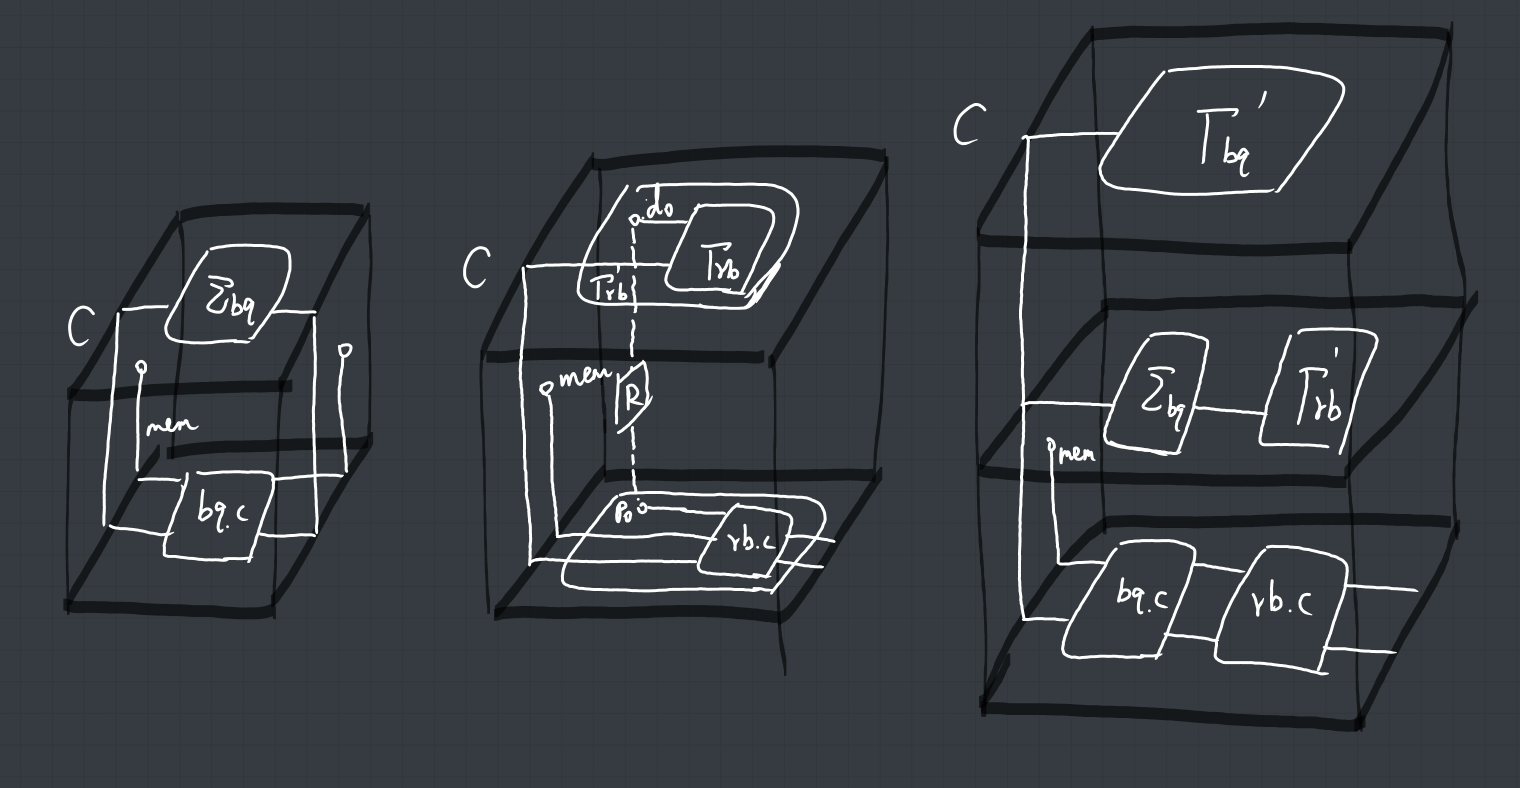
\includegraphics[scale=0.09]{./pr/bq-example.png}}
  \]
  \caption{todo}
  \label{fig:bq-example}
\end{figure}

It is noticable from the previous section that
the simulation convention for $\phi'_3$
is unwieldy because the program $\kw{rb.c}$
implements the state $D_\kw{rb}$ using its memory state.
To facilitate the verification of such programs,
we exploit memory separation from \S\ref{sec:overview:sepalg}
to split the memory data that implements the abstract state
from the entire memory.
Thus, we introduce ClightP
\[
  \kw{ClightP}(M) :
    \mathcal{C} \mathbin@ \kw{mem}
    \twoheadrightarrow
    \mathcal{C} \mathbin@ \kw{mem} \mathbin@ \kw{penv}
  \,,
\]
a variant of Clight
where global variables can be declared \emph{private}.
Private variables cannot be accessed
from other translation units and are stored
in a separate
\emph{private environment} $p \in \kw{penv}$.
The program $M$ can easily be compiled to a regular
Clight program $M' := \kw{ClightUnP}(M)$
by erasing the $\kw{private}$ annotations from all variables.

We define a version
$\kw{ClightP}\langle M \rangle :
    \mathcal{C} \mathbin@ \kw{mem} \rightarrow
    \mathcal{C} \mathbin@ \kw{mem}$
of the ClightP semantics
which encapsulates the private environment, as
\[
  \kw{ClightP} \langle M \rangle := \:
  \begin{tikzpicture}[xscale=0.35,yscale=0.17,baseline=(m.base)]
    % Background
    \fill[tssdbg] (1,-2) rectangle (11,6.5);
    \fill[pattern=north east lines] (1,-2) rectangle (11,0);
    % Wires
    \draw (1,0) node[left] {$\mathcal{C}$}
      -- (11,0) node[right] {$\mathcal{C}$};
    \draw (1,2) node[left] (m) {$\kw{mem}$}
      -- (11,2) node[right] {$\kw{mem}$};
    \draw (3,4)
        node[circle,inner sep=1pt,draw,fill=white] {}
        node[left] {$p_0$}
        -- (4,4);
    % Boxes
    \draw[fill=white,rounded corners]
      ( 4,-1) rectangle (10,5) node[midway] (N) {$\kw{ClightP}(M)$};
  \end{tikzpicture} \: =
  (\mathcal{C} \mathbin@ \kw{mem} \mathbin@ [ p_0 \rangle) \odot
    \kw{ClightP}(M)
  \,,
\]
where
$p_0 := \kw{init\_penv}(M)$
is the initial state of the private environment.
Note that the resulting type
means that ClightP semantics in this form
can be composed directly.

\begin{example}[Verifying $\kw{rb.c}$]
Using ClightP for $\kw{rb.c}$,
we can declare the variables
\texttt{c1}, \texttt{c2} and \texttt{buf}
as private.
The correctness can be stated as follows:
\[
  \psi_\kw{rb} \: : \: \Gamma'_\kw{rb}
    \le_{\varnothing \twoheadrightarrow
      \mathcal{C} \mathbin@ \langle \kw{mem} ]^*}
    \kw{ClightP}\langle \kw{rb.c} \rangle
\]
As shown in Figure~\ref{fig:bq-example}(b),
the relation
$R_\kw{rb} \subseteq D_\kw{rb} \times \kw{penv}$
becomes hidden,
and the interface is simplified
so that it is easier to compose.
The compilation phase,
as we will see shortly,
takes care of the step that
translates the $\kw{penv}$ further down to the memory.

Again,
by composing the individual proofs together,
the complete proof can be obtained:
\[
\psi_\kw{bq} \: : \:
\Gamma'_\kw{bq} \le_{\varnothing \twoheadrightarrow
      \mathcal{C} \mathbin@ \langle \kw{mem} ]^*}
    \kw{ClightP}(\kw{bq.c}) \odot \kw{ClightP}(\kw{rb.c})
    \: := \:
    todo
\]
The complete proof is shown in Figure~\ref{fig:bq-example}(c).

\end{example}

\paragraph{Correctness Property}
We now discuss the correctness of
the transformation $\kw{ClightUnP}$
which converts private variables into regular variables
stored in the global memory state.
The corresponding correctness property is
formulated using the techniques outlined in \S\ref{sec:overview:sepalg} as
\[
\kw{ClightP}\langle M \rangle \le_{\mathcal{C}@(\kw{mem} @ \langle \kw{mem} ]_*;\bullet) \twoheadrightarrow \mathcal{C}@(\kw{mem} @ [ \kw{m_0} \rangle_*;\bullet)} \kw{Clight}(M')
\]
The correctness property
can be decomposed as shown in Figure~\ref{fig:clightp-correct},
where the relation $R_p \subseteq \kw{penv} \times \kw{mem}$
connects the private environment and the memory.

\begin{figure}
  \[
    \text{(a)}
    \qquad
    \raisebox{-0.5\height}{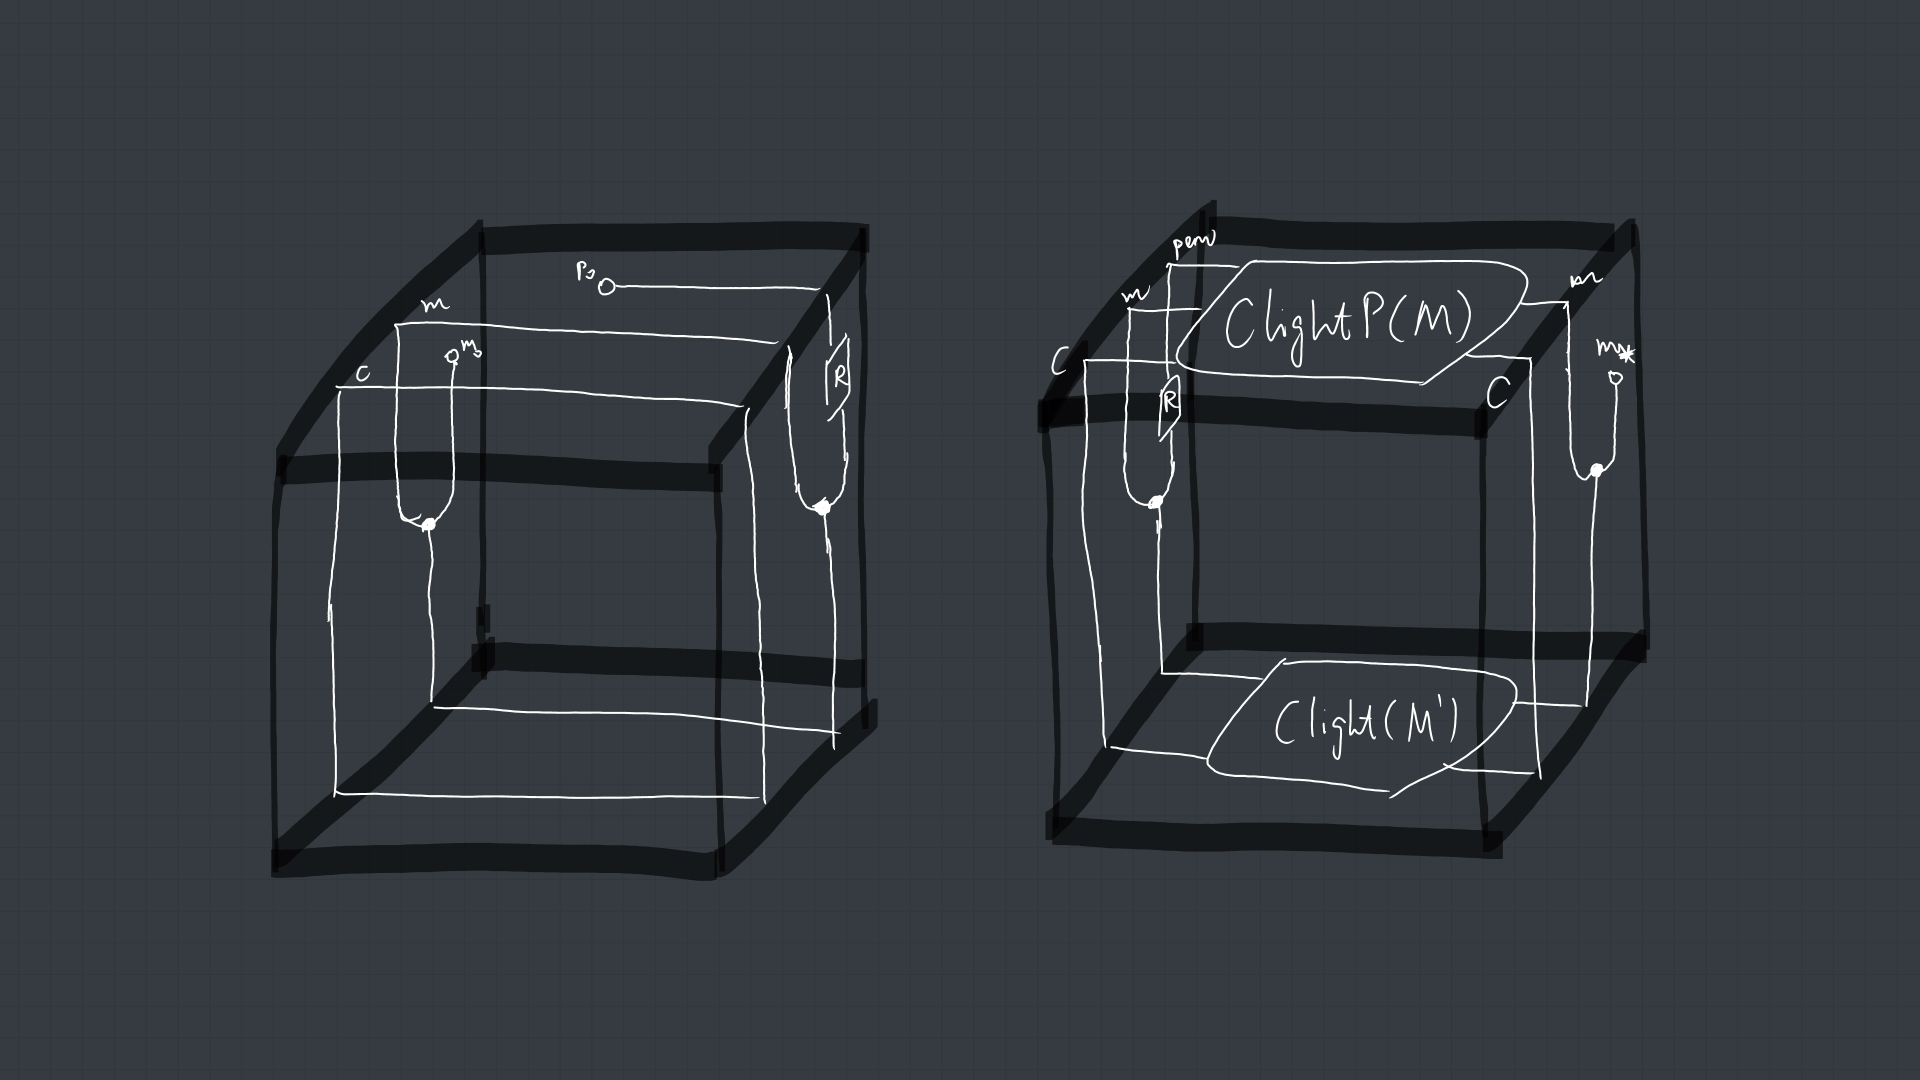
\includegraphics[scale=0.09]{./pr/clightp.jpg}}
    \qquad
    \text{(b)}
    \qquad
    \raisebox{-0.5\height}{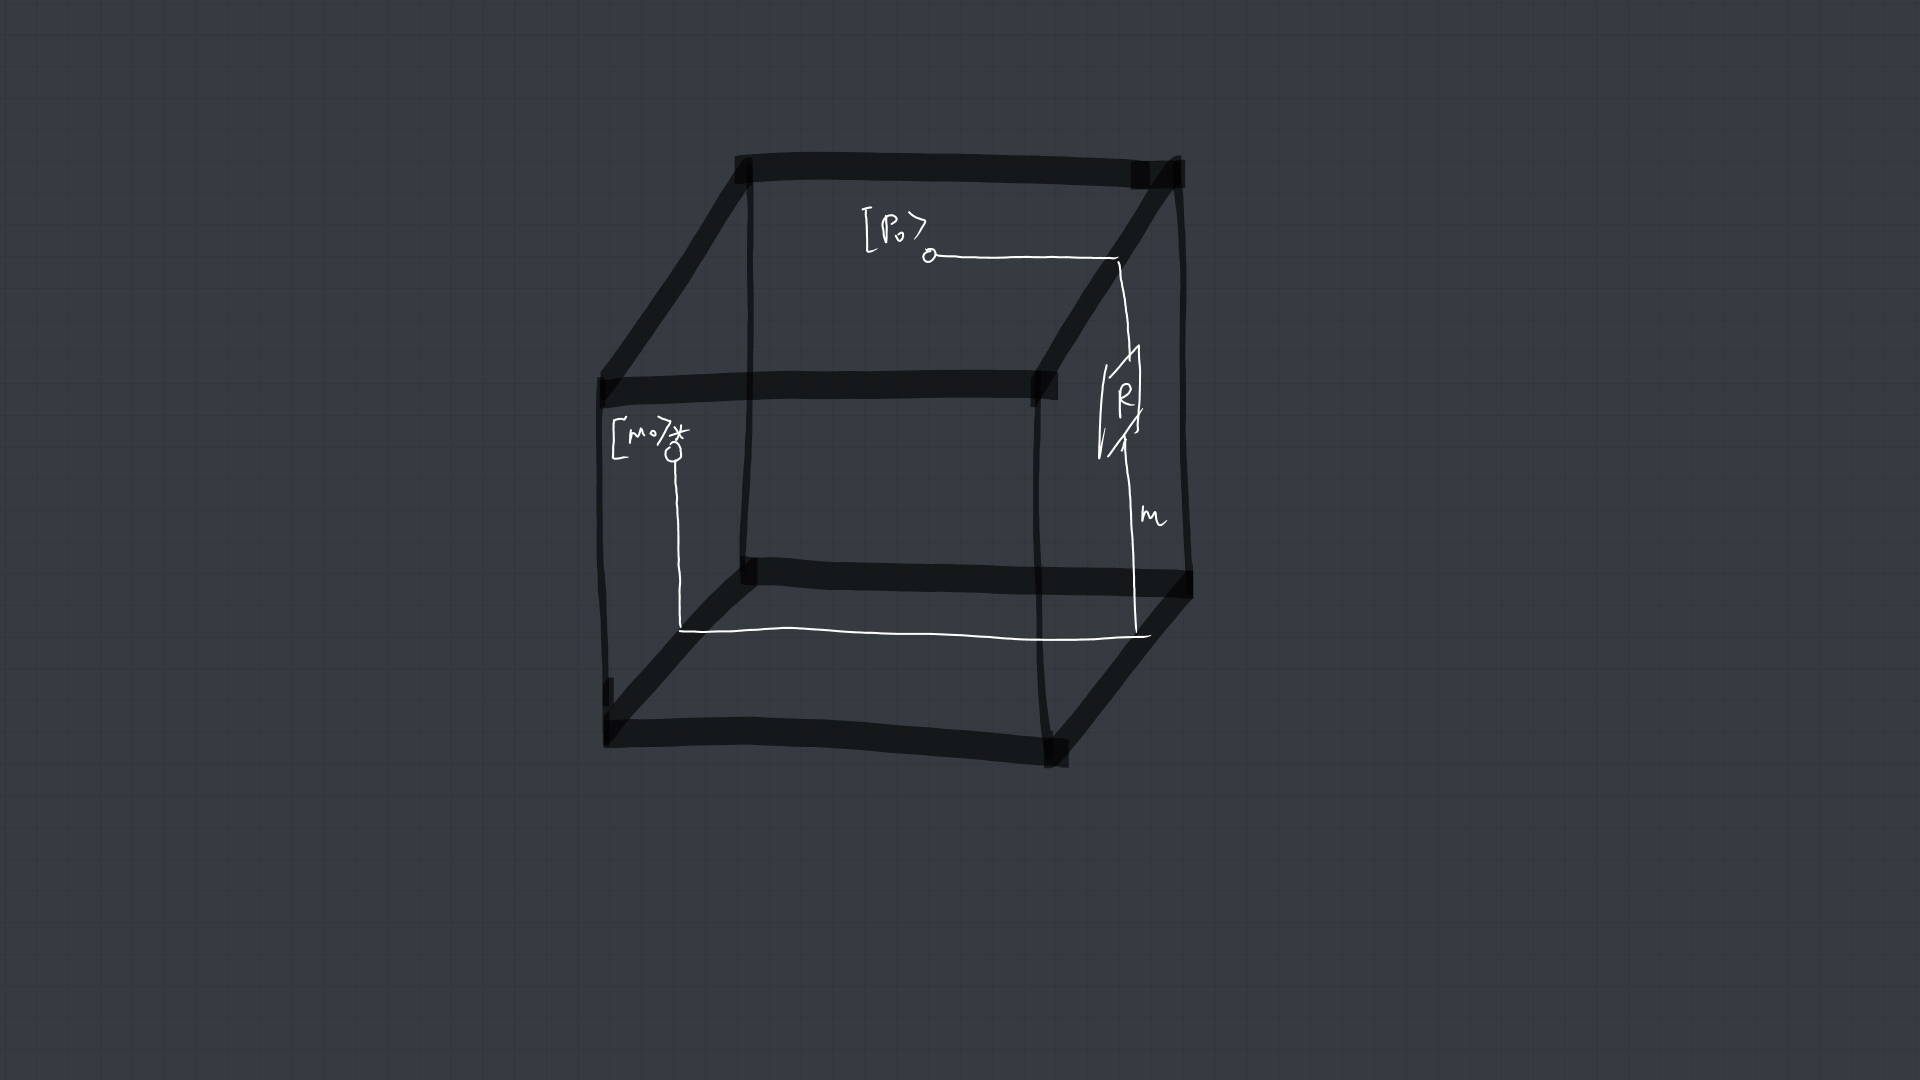
\includegraphics[scale=0.09]{./pr/clightp-rel.jpg}}
  \]
  \caption{todo}
  \label{fig:clightp-correct}
\end{figure}

\paragraph{Composition}
todo

%}}}

\subsection{Certified Abstraction Layers} \label{sec:application:cal} %{{{

Certified abstraction layers (CAL) framework
provides a theoretical foundation
for large scale system verification,
by allowing
the high-level abstract specification
to be progressively refined
through a series of abstraction layers.
The correctness of individual components is denoted by
\[
  L^\sharp \vdash_R M : L^\flat,
\]
which says that
the behavior of an overlay specification $L^\sharp: \top \twoheadrightarrow \mathcal{C} @ D^\sharp$
is refined by an implementation $M: \mathcal{C} \mathbin@ \kw{mem} \twoheadrightarrow \mathcal{C} \mathbin@ \kw{mem}$
executed on top of an underlay $L^\flat: \top \twoheadrightarrow \mathcal{C} @ D^\flat$
witnessed by the abstraction relation $R \subseteq D^\sharp \times (\kw{mem} \times D^\flat)$.

With the state encapsulation,
we can define encapsulated layer interfaces:
\[
  \Gamma^\sharp := (\mathcal{C} \mathbin@ [ d^\sharp_0 \rangle ) \odot L^\sharp : \top \twoheadrightarrow \mathcal{C} \qquad
  \Gamma^\flat := (\mathcal{C} \mathbin@ [ d^\flat_0 \rangle ) \odot L^\flat : \top \twoheadrightarrow \mathcal{C}
\]
and use the $\kw{ClightP}$ semantics
to interpret the abstraction layers:
\[
  L^\sharp \vdash M : L^\flat \: :\Leftrightarrow \: \Gamma^\sharp \mathbin@ \kw{mem} \le \kw{ClightP}\langle M \rangle \odot (\Gamma^\flat \mathbin@ \kw{mem})
\]
as shown in Figure~\ref{fig:cal}.
Note that the abstraction relation
$R \subseteq D^\sharp \times (\kw{penv} \times D^\flat)$ is hidden,
and abstraction layers compose naturally.

\begin{figure}
  \[
    \raisebox{-0.5\height}{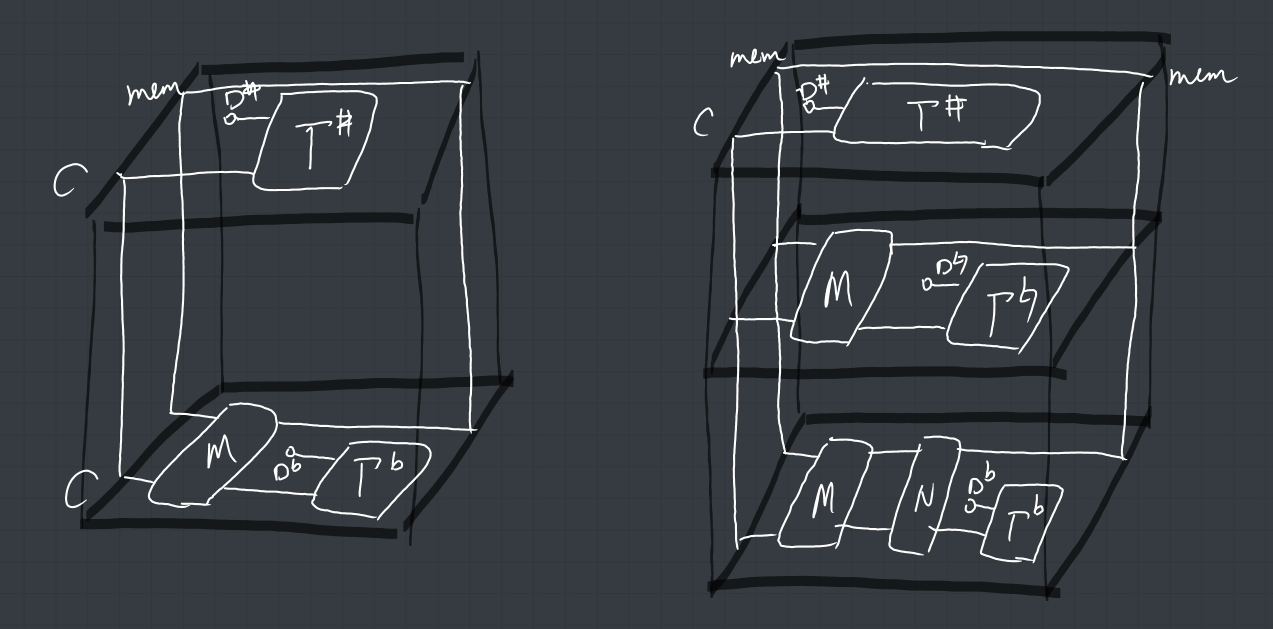
\includegraphics[scale=0.09]{./pr/cal.png}}
  \]
  \caption{todo}
  \label{fig:cal}
\end{figure}

It is worth mentioning that
the example of ring buffer and bounded queue
are special cases of certified abstraction layers
in that
the ring buffer layer is built on top of an empty underlay,
and the implementation of the bounded queue layer
does not introduce state.

%}}}

% {
% \color{gray}

% \subsection{Clight with module-local state} \label{sec:application:clightp} %{{{

% We have briefly introduced in \S\ref{sec:overview:clightp}
% the language ClightP which allows \emph{private} variables
% to be stored in a separate environment.
% We now discuss the correctness of
% the transformation $\kw{ClightUnP}$
% which converts private variables into regular variables
% stored in the global memory state.
% The corresponding correctness property is
% formulated using the techniques outlined in \S\ref{sec:overview:sepalg}.

% \paragraph{Correctness Property}

% Given a simulation convention $\mathbf{R} : A \leftrightarrow \kw{mem}$,
% we write $\mathbf{R}^\bullet :=
% (\kw{mem} \otimes \mathbf{R}) \mathbin; [\bullet] :
%  \kw{mem} \otimes A \leftrightarrow \kw{mem}$
% for the simulation convention
% which merges the target memory share of $\mathbf{R}$
% into another memory component.
% In addition,
% the simulation convention $[U]_* : \mathbf{I} \leftrightarrow U$
% allows the caller to use an arbitrary target question $u$
% but requires the callee to return it unchanged.
% The correctness of $\kw{ClightUnP}$
% can then be stated as:
% \[
%   \begin{tikzpicture}[xscale=0.35,yscale=0.4,baseline=2em]
%      \footnotesize
%      % Background
%      \fill[scsdbg] (-1,0) rectangle (5.3,4);
%      % Content
%      \draw (0,4)
%         -- (0,0) coordinate (C2);
%      \draw[rounded corners]
%           (2,4) node[above,xshift=1ex,overlay] (m1)
%             {$\mathcal{C} \mathbin@ \kw{mem} \mathbin@ \kw{penv}$}
%        -- (2,2) -- (3,1);
%      \draw[rounded corners] (4,4)
%        -- (4,2.8) node[draw,fill=white] {$R_\kw{P}$}
%        -- (4,2) -- (3,1);
%      \draw (3,1) node {$\bullet$}
%        -- (3,0) coordinate (m2);
%      \path (C2) -- (m2) node[midway,below,xshift=0.5ex]
%        {$\mathcal{C}\:\:\,\mathbin@\:\:\,\kw{mem}$};
%   \end{tikzpicture}
%   \begin{tikzpicture}[xscale=0.75,yscale=0.4,baseline=2em]
%      % Background
%      \fill[memsdbg] (0,0) rectangle (6,4);
%      \fill[penvsdbg] (0,2) rectangle (3,4);
%      %\fill[pattern=crosshatch dots,opacity=0.2] (0,2) rectangle (3,4);
%      \node[below right,opacity=0.5,inner sep=2pt] at (0,4)
%        {\scriptsize $C \mathbin@ \kw{mem} \mathbin@ \kw{penv}$};
%      \node[above right,opacity=0.5,inner sep=2pt] at (0,0)
%        {\scriptsize $C \mathbin@ \kw{mem}$};
%      \node[below left,opacity=0.5,inner sep=2pt] at (6,4)
%        {\scriptsize $C \mathbin@ \kw{mem}$};
%      \node[above left,opacity=0.5,inner sep=2pt] at (6,0)
%        {\scriptsize $C \mathbin@ \kw{mem}$};
%      %
%      \footnotesize
%      \draw (0,2) node[left] {${} = \mathcal{C} \otimes [R_\kw{P}]^\bullet$}
%         -- (6,2) node[right] {$\mathcal{C} \otimes [\kw{mem}]_*^\bullet = {}$};
%      \draw (3,4) node[above] {$\kw{ClightP}(M)$}
%         -- (3,0) node[below] {$\kw{Clight}(M')$};
%      \node[draw,rounded corners,fill=white] at (3,2)
%        {\normalsize $\kw{ClightUnP}$};
%   \end{tikzpicture}
%   \begin{tikzpicture}[xscale=0.35,yscale=0.4,baseline=2em]
%      \footnotesize
%      % Background
%      \fill[scsdbg] (-0.5,0) rectangle (6,4);
%      % Edges
%      \draw (0.5,4) coordinate (C1)
%         -- (0.5,0) coordinate (C2);
%      \draw[rounded corners]
%           (2,4) coordinate (m1)
%        -- (2,2) -- (3,1);
%      \draw[rounded corners]
%           (4,3) node[draw,fill=white] {$[\kw{mem}]_*$}
%        -- (4,2) -- (3,1);
%      \draw (3,1) node {$\bullet$}
%        -- (3,0) coordinate (m2);
%      \path (C1) -- (m1) node[midway,above,xshift=1ex]
%        {$\mathcal{C} {\mathbin@} \kw{mem}$};
%      \path (C2) -- (m2) node[midway,below,xshift=0.75ex]
%        {$\mathcal{C} \: \mathbin@ \: \kw{mem}$};
%   \end{tikzpicture}
% \]
% The Clight program
% stores formerly private variables in the main memory.
% For incoming calls,
% the private environment is refined
% into a memory share according to a relation $R_\kw{P}$,
% which is then incorporated into the main memory.
% For outgoing calls,
% the private environment is not included in the source question,
% but the corresponding variables are part of the target memory.
% The use of $[\kw{mem}]_*^\bullet$
% requires the callee to return
% this region of the memory unchanged.

% \paragraph{Encapsulating Private Environments}

% In order to give the semantics
% a more tractable type,
% we can encapsulate the private environment:
% \[
%   \kw{ClightP} \langle M \rangle :=
%     (C \mathbin@ \kw{mem} \mathbin@ \langle p_0 \rangle) \odot
%     \kw{ClightP}(M)
%     :
%     \mathcal{C} \mathbin@ \kw{mem} \twoheadrightarrow
%     \mathcal{C} \mathbin@ \kw{mem}
% \]
% Here $p_0 := \kw{init\_penv}(M)$ is the initial private environment for $M$.
% The facilities discussed in \S\ref{sec:overview:encap}
% can then be used to
% derive a correctness property
% stated in terms of the encapsulated semantics:
% \[
%   \begin{tikzpicture}[xscale=0.60,yscale=0.3]
%     % Background
%     \fill[memsdbg] (0,11) -- (2,11)
%       [rounded corners] -- (2,6)
%       [sharp corners] -| cycle;
%     \fill[penvsdbg] (2,11) rectangle (6,8);
%     \fill[memsdbg] (6,11) rectangle (9,8);
%     \fill[mmemsdbg] (0,6)
%       [rounded corners] -- (2,6)
%       [sharp corners] |- (9,8) -- (9,3) -| cycle;
%     \fill[memsdbg] (0,3) rectangle (9,0);
%     % Region labels
%     \begin{scope}[opacity=0.5,inner sep=2pt]
%       \scriptsize
%       \node[below right,xshift=-1pt] at (0,11) {$\mathcal{C} \mathbin@ \kw{mem}$};
%       \node[above right] at (0,0) {$\mathcal{C} \mathbin@ \kw{mem}$};
%       \node[below left] at (9,11) {$\mathcal{C} \mathbin@ \kw{mem}$};
%       \node[above left] at (9,0) {$\mathcal{C} \mathbin@ \kw{mem}$};
%       \node[below] at (4,11) {$\mathcal{C} \mathbin@ \kw{mem} \mathbin@ \kw{penv}$};
%       \node[right] at (0,4.5) {$\mathcal{C} \mathbin@ \kw{mem} \mathbin@ \kw{mem}$};
%     \end{scope}
%     % Wires
%     \begin{scope}
%       \footnotesize
%       \draw (2,11)
%         node[above] (x) {$(\mathcal{C} \mathbin@ \kw{mem} \mathbin@ \langle p_0 \rangle)$}
%         [rounded corners] -- (2,6) [sharp corners] -- (0,6)
%         node[left] {$\mathcal{C} \mathbin@ \kw{mem} \otimes \langle m_0 \rangle_*$};
%       \draw (6,11) node[above] (y) {$\kw{ClightP}(M)$}
%         -- (6,0) node[below] {$\kw{Clight}(M')$};
%       \draw (2,8) -- (9,8) node[right]
%         {$\mathcal{C} \mathbin@ \kw{mem} \otimes [\kw{mem}]_*$};
%       \draw (0,3) node[left] {$\mathcal{C} \mathbin@ {\bullet}$}
%         -- (9,3) node[right] {$\mathcal{C} \mathbin@ {\bullet}$};
%       \path (x) -- (y) node[midway] {$\odot$};
%     \end{scope}
%     % Components
%     \node[draw,fill=white,rounded corners] at (2,8) {$p_0 \mathrel{R_\kw{P}} m_0$};
%     \draw[fill=white,rounded corners] (4,2) rectangle (8,9)
%       node[midway] {$\kw{ClightUnP}$};
%   \end{tikzpicture}
% \]
% Here, $m_0 := \kw{init\_mem} \big(M'_\kw{priv}\big)$
% is the initial memory fragment associated with
% the global variable definitions introduced in $M'$
% in order to implement the private variables of $M$.
% Note that private environments
% no longer appear in the type of the ClightP semantics
% or in the correctness property.

% \paragraph{Composition}

% One challenge is that the correctness property depicted above
% is not compositional,
% because the incoming and outgoing simulation conventions are different:
% \[
%     \kw{ClightP}\langle M \rangle
%       \le_{\mathcal{C} \otimes [\kw{mem}]_*^\bullet
%            \twoheadrightarrow
%            \mathcal{C} \otimes \langle m_0 \rangle_*^\bullet}
%       \kw{Clight}(M')
% \]
% Two ClightP modules
% $
%   \kw{ClightP} \langle M_1 \rangle \odot \kw{ClightP}\langle M_2 \rangle
% $
% can be composed,
% but the associated $\kw{ClightUnP}$ correctness properties
% do not directly compose alongside them.
% We will use the following strategy:
% \[
%   \begin{tikzpicture}[xscale=0.7,yscale=0.6]
%     \fill[memsdbg] (0,0) rectangle (11,4);
%     % Region label
%     \begin{scope}[opacity=0.5,inner sep=2pt]
%       \scriptsize
%       \node at (5.5,2) {$\mathcal{C} \mathbin@ \kw{mem}$};
%     \end{scope}
%     % Strings
%     \begin{scope}
%       \footnotesize
%       \draw (4,4) node[above] (S1) {$\kw{ClightP}\langle M_1 \rangle$}
%          -- (4,0) node[below] (T1) {$\kw{Clight}(M_1')$};
%       \draw (7,4) node[above] (S2) {$\kw{ClightP}\langle M_2 \rangle$}
%          -- (7,0) node[below] (T2) {$\kw{Clight}(M_2')$};
%       \path (S1) -- (S2) node[midway] {$\odot$};
%       \path (T1) -- (T2) node[midway] {$\odot$};
%       \draw (0,2) node[left] {$\langle m_0^1 \bullet m_0^2 \rangle^\bullet_*$}
%         -- (1,2)
%         [rounded corners] -- (2,3)
%         node[above left,inner sep=0pt]
%           {\scriptsize $\langle m_0^1 \rangle_*^\bullet$}
%         -- (9,3)
%         node[above right,inner sep=0pt]
%           {\scriptsize $[\kw{mem}]_*^\bullet$}
%         [sharp corners] -- (10,2)
%         -- (11,2) node[right] {$[\kw{mem}]_*^\bullet$};
%       \draw (1,2)
%         [rounded corners] -- (2,1)
%         node[below left,inner sep=0pt]
%           {\scriptsize $\langle m_0^2 \rangle_*^\bullet$}
%         -- (9,1)
%         node[below right,inner sep=0pt]
%           {\scriptsize $[\kw{mem}]_*^\bullet$}
%         [sharp corners] -- (10,2);
%     \end{scope}
%     % Numbered nodes
%     \begin{scope}[every node/.style={draw,circle,fill=white,inner sep=2pt}]
%       \small
%       \node at (1,2) {3};
%       \node at (4,1) {2};
%       \node at (7,3) {1};
%       \node at (10,2) {4};
%     \end{scope}
%     % ClightUnP nodes
%     \begin{scope}[every node/.style={draw,rounded corners,fill=white}]
%       \small
%       \node at (4,3) {$\kw{ClightUnP}$};
%       \node at (7,1) {$\kw{ClightUnP}$};
%     \end{scope}
%   \end{tikzpicture}
% \]
% First,
% we will establish self-simulation properties
% for $\kw{ClightP}$ (1) and $\kw{Clight}$ (2)
% which show that they are compatible with
% the simulation conventions
% $[\kw{mem}]_*^\bullet$
% and $\langle m \rangle_*^\bullet$.
% These properties follow mainly from the frame rule
% of our memory separation primitives.
% Second,
% we show that the incoming (3) and outgoing (4)
% simulation conventions compose with themselves.

% First,
% the property
% $
%   \kw{Clight}(M)
%   \le_{\langle m \rangle_*^\bullet \twoheadrightarrow \langle m \rangle_*^\bullet}
%   \kw{Clight}(M)
% $,
% stems from the fact that
% \[
% L \odot (A \mathbin@ \langle u \rangle) = L \mathbin@ \langle u \rangle =
%  (B \mathbin@ \langle u \rangle) \odot (L \mathbin@  U)
%   \quad\text{for any}  \quad L : A \twoheadrightarrow B
%   \,.
% \]
% This can be combined with the frame rule and properties of $\langle m_0 \rangle_*$ to show:
% \[
%   \begin{tikzpicture}[xscale=0.5,yscale=0.3]
%     % Background
%     \begin{scope}
%       \fill[memsdbg] (0,10) -- (0,4)
%         [rounded corners] -- (2,4) -- (2,5) -- (4,7) -- (4,8)
%         [sharp corners] -- (6,8) |- cycle;
%       \fill[mmemsdbg] (0,2) -- (0,4)
%         [rounded corners] -- (2,4) -- (2,5) -- (4,7) -- (4,8)
%         [sharp corners] -- (6,8) |- cycle;
%       \fill[memsdbg] (0,0) rectangle (6,2);
%     \end{scope}
%     % Region labels
%     \begin{scope}[opacity=0.5,inner sep=2pt]
%       \tiny
%       \node[below right] at (0,4)
%         {$\mathcal{C} \mathbin@ \kw{mem} \mathbin@ \kw{mem}$};
%       \node[below left] at (6,10)
%         {$\mathcal{C} \mathbin@ \kw{mem}$};
%       \node[above right] at (0,0)
%         {$\mathcal{C} \mathbin@ \kw{mem}$};
%     \end{scope}
%     % Strings
%     \begin{scope}
%       \footnotesize
%       \draw (2,10) node[above] {$\kw{Clight}(M)$}
%         [rounded corners] -- (2,7) -- (4,5)
%         node[below right] {\tiny $\kw{Clight}(M) \mathbin@ \kw{mem}$}
%         [sharp corners] -- (4,0)
%         node[below] {$\kw{Clight}(M)$};
%       \draw (0,4) node[left]
%           {$\mathcal{C} \mathbin@ \kw{mem} \otimes \langle m_0 \rangle_*$}
%         [rounded corners] -- (2,4) -- (2,5) -- (4,7) -- (4,8)
%         [sharp corners] -- (6,8) node[right]
%           {$\mathcal{C} \mathbin@ \kw{mem} \otimes \langle m_0 \rangle_*$};
%       \draw (0,2) node[left] {$\mathcal{C} \mathbin@ {\bullet}$}
%         -- (6,2) node[right] {$\mathcal{C} \mathbin@ {\bullet}$};
%     \end{scope}
%     % Nodes
%     \begin{scope}[every node/.style={draw,fill=white}]
%       \node[circle,inner sep=2pt] at (3,6) {$=$};
%       \node[rounded corners] at (4,2) {$\kw{Frame}$};
%     \end{scope}
%   \end{tikzpicture}
% \]
% A similar argument can be used to show
% the analogous property of ClightP.

% Second,
% the self-composition of the simulation conventions involved
% follows mostly from properties of the partial commutative monoid.

% %}}}

% \subsection{Ad-hoc Verification} \label{sec:application:ad-hoc}

% We have already seen in \S\ref{sec:overview}
% that states have to be explicitly attached to transition systems
% in order to identify the interfaces across different components.
% It immediately becomes overwhelming,
% and great care have to be taken
% in order to put together all the pieces correctly.
% In contrast,
% once the states in the specifications
% are encapsulated by defining
% \[
%   \Gamma_\kw{bq}: \top \rightarrow \mathcal{C} := (\epsilon \in \kw{val}^* \mid L_\kw{bq}) \qquad
%   \Gamma_\kw{rb}: \top \rightarrow \mathcal{C} := ((\bot, 0, 0) \in \kw{val}^N \times \mathbb{N} \times \mathbb{N} \mid L_\kw{rb}),
% \]
% and the static variables in the $\kw{Clight}$ programs are
% converted to private ones
% \[
%   \kw{ClightP} \langle \kw{bq.cp} \rangle : \mathcal{C} @ \kw{mem} \rightarrow \mathcal{C} @ \kw{mem} \qquad
%   \kw{ClightP} \langle \kw{rb.cp} \rangle : \mathcal{C} @ \kw{mem} \rightarrow \mathcal{C} @ \kw{mem},
% \]
% the interfaces across different components are identified
% except for an innocent memory state to be passed through.
% With the individual correctness
% \[
%   \pi_\kw{bq}:\ \Gamma_\kw{bq} \le \Sigma_\kw{bq} \circ \Gamma_\kw{rb} \qquad
%   \pi_\kw{bq'}:\ \Sigma_\kw{bq} @ \kw{m} \le \kw{ClightP}\langle \kw{bq.cp} \rangle \qquad
%   \pi_\kw{rb}:\ \Gamma_\kw{rb} @ \kw{m} \le \kw{ClightP} \langle \kw{rb.cp} \rangle
% \]
% the complete proof can be presented
% as a string diagram in Figure~\ref{fig:application:example}.


% \subsection{Certified Abstraction Layers} \label{sec:application:cal}

% Certified abstraction layers (CAL) framework
% provides a theoretical foundation
% for large scale systems verification,
% by allowing
% the high-level abstract specification
% to be progressively refined
% through a series of abstraction layers.
% The correctness of individual components is denoted by
% \[
%   L^\sharp \vdash_R M : L^\flat,
% \]
% which says that
% the behavior of an overlay specification $L^\sharp: \top \twoheadrightarrow \mathcal{C} @ D^\sharp$
% is refined by an implementation $M: \mathcal{C} \twoheadrightarrow \mathcal{C}$
% executed on top of an underlay $L^\flat: \top \twoheadrightarrow \mathcal{C} @ D^\flat$
% witnessed by the abstraction relation $R \subseteq D^\sharp \times D^\flat$.
% Abstraction layers are composed according to the following rule
% \[
%   \begin{prooftree}
%     \hypo{L^\natural \vdash_R M : L^\sharp}
%     \hypo{L^\flat \vdash_S N : L^\natural}
%     \infer2{L^\flat \vdash_{R \circ S} M + N : L^\sharp}
%   \end{prooftree}
% \]

% However, there lacks a satisfying instance of the framework.
% The closest one uses CompCertX with primitives
% to implementation the semantics of the framework,
% where the layer correctness is interpreted as
% (roughly expressed using our notations)
% \[
%   L^\sharp \vdash_R M : L^\flat :\Leftrightarrow L^\sharp @ \kw{mem} \le_{\varnothing \twoheadrightarrow [R]} \kw{ClightX}_{L^\flat @ \kw{mem}} [M],
% \]
% where $\kw{ClightX_L[M]}$ interprets
% a module $M$ of Clight functions
% with external calls being interpreted
% according to the underlay interface $L$,
% and the simulation relation $[R] \subseteq (D^\sharp \times \kw{mem}) \times (D^\flat \times \kw{mem})$
% allows the abstract state to be realized
% by concrete memory state.
% Memory injection is used so that the abstraction layers
% are composible to the CompCertX compiler.

% Although it has been applied to verify CertiKOS,
% the above framework has two major limitations.
% On one hand,
% the $\kw{ClightX}$ semantics is not truly open
% in that the behaviors of external calls have to be provided by the underlay.
% As a consequence,
% the process of layer construction requires
% the well-formedness of the underlay.
% On the other,
% the composition on abstraction relations
% becomes much complicated
% when it incorporates the memory injection.

% By contrast, with CompCertO semantics and the state encapsulation,
% the abstraction relation can be encapsulated,
% which gives a simpler interpretation of the abstraction layers:
% \[
%   L^\flat \vdash M : L^\sharp :\Leftrightarrow L^\sharp @ \kw{mem} \le \kw{ClightP} \langle M \rangle \circ L^\flat @ \kw{mem}
% \]
% The truly openness of CompCertO semantics
% enables modules to be verified independent of underlay semantics.
% For example, the program $\kw{bq.cp}$ is verified
% with reference to its specification $\Sigma_\kw{bq}$
% without relying on any underlay specifications.
% Moreover,
% since the abstract relation has been encapsulated,
% the vertical composition of certified abstraction layers
% can be established as a corollary of
% the vertical composition of encapsulated semantics.
% Furthermore,
% with the ability of combining memory fragments,
% a form of horizontal composition of
% abstraction layers can be established
% in a straightforward way,
% which would be complicated due to
% the intricacy between the abstraction relation
% and the memory state.

% \subsection{Future Work}

% Talk about mixing C and assembly semantics
% using the notions of companion/conjoint
% for the compiler's simulation convention.
% Assuming a demonic interpretation for CompCert's transition systems,
% by adapting
% the techniques used for CompCertM's \emph{repaired interaction semantics} of assembly,
% it might be possible to define
% \[
%   \mathcal{CA} : \mathcal{A} \twoheadrightarrow \mathcal{C}
%   \qquad \text{and} \qquad
%   \mathcal{AC} : \mathcal{C} \twoheadrightarrow \mathcal{A}
%   \,,
% \]
% so that repaired interaction semantics boil down to:
% \[
%   \kw{Asm}_\mathcal{C}(M) := \mathcal{CA} \odot \kw{Asm}(M) \odot \mathcal{AC}
%     : \mathcal{C} \twoheadrightarrow \mathcal{C}
%   \,.
% \]
% We could then try to establish properties like:
% \[
%   \kw{id}_\mathcal{C}
%   \le_{\mathbb{C} \twoheadrightarrow \mathcal{C}}
%   \mathcal{CA}
%   \le_{\mathcal{A} \twoheadrightarrow \mathbb{C}}
%   \kw{id}_\mathcal{A}
%   \qquad
%   \kw{id}_\mathcal{C}
%   \le_{\mathcal{C} \twoheadrightarrow \mathbb{C}}
%   \mathcal{AC}
%   \le_{\mathbb{C} \twoheadrightarrow \mathcal{A}}
%   \kw{id}_\mathcal{A}
% \]

% }

%}}}

\section{Related Work} %{{{

\subsection{CompCert-based Vertification Frameworks}

CompCert \cite{compcert}
is the first certified C compiler offering industrial-grade performance,
and there are many verification frameworks which connect with the compiler
to offer formal guarantees going all the way to assembly code.
For example, VST \cite{vst}
provides a separation logic for Clight,
and includes a soundness proof which interfaces with CompCert's correctness proof.

\paragraph{Compositional Semantics}

Compositional semantics were introduced by
Compositional CompCert \cite{compcompcert}
in part to support the verification of
programs with multiple translation units,
potentially written in different languages.
However,
this model uses a fixed language interface and simulation convention.
CompCertM \cite{compcertm} refined this approach
with a better model of the interaction between
C and assembly programs,
and more flexibility in simulation conventions.
Notably,
this makes it possible to introduce module-local state
by expressing constraints on the environment.
However, neither Compositional CompCert nor CompCertM
support data abstraction or state encapsulation
of the kinds we have presented,
and the general notions of
language interface and simulation convention
were first introduced in CompCertO.
We refer interested readers to \citet{compcerto}
for a detailed comparison between Compositional CompCert,
CompCertM and CompCertO.

Interaction trees \cite{itree,itrees} provide
another framework for compositional semantics
formalized in the Coq proof assistant
which presents similarities with our own,
though their interface with CompCert is less comprehensive.

\paragraph{Certified Abstraction Layers}

Data abstraction in a form closer to our own
is present in certified abstraction layers (CAL),
originally implemented by CompCertX \cite{popl15}
to verify the certified operating CertiKOS.
Expressed in our framework,
the semantic model of CompCertX can be summarized as
\[
  \forall D^\flat \in \mathbf{Set}
  \: \mathbin. \:
  L^\flat :
    \top \twoheadrightarrow
    \mathcal{C} \mathbin@ \kw{mem} \mathbin@ D^\flat
  \: \vdash \:
  \kw{Clight}_{L^\flat}[M] :
    \top \twoheadrightarrow
    \mathcal{C} \mathbin@ \kw{mem} \mathbin@ D^\flat
  \,.
\]
Here $L^\flat$ is an \emph{underlay interface}.
The goal is to implement an \emph{overlay}
$
  L^\sharp \le_{\top \twoheadrightarrow \mathcal{C}@R}
    \kw{Clight}_{L^\flat}[M]
$,
in a way which allows an abstraction relation
$R \subseteq (\kw{mem} \times L^\sharp) \times (\kw{mem} \times L^\flat)$
to refine and augment the abstract data component.
Layers verified in this way can then be combined sequentially.

Subsequent work has extended CAL to support concurrency \cite{ccal}.
The original model is tied to the CompCert semantics but
further work explores more abstract versions \cite{rbgs-cal,popl22}.
In particular a version of the $\mathbin@$ construction appears in \citet{rbgs-cal}.
However, these more abstract frameworks
have not been implemented.

\subsection{Langauge-Agnostic Verification Framework}

\paragraph{Contextual Conditional Refinement}

The contextual conditional refinement(CCR)\cite{ccr}
combines refinement and separation logic
into a unified framework,
so that it enjoys both
pre- and post-condition style of reasoning from separation logic
and transitive composition of layer refinements.
There are two remarkable differences between CCR and our framework.
First, CCR does not support state encapsulation,
meaning that the client has to be aware of
the representation of the component's state
in order to achieve contextual refinement.
That said, the usage of separation logic in CCR
allows for local reasoning on the state to some extent.
Second, the source- and target-level specifications
in CCR have to agree on the same calling convention.
By contrast,
our framework is capable of
establishing the refinement between
specifications using different calling conventions
through simulation conventions,
which allows for more flexibility.

\subsection{Categorical Structures}

To our knowledge,
the work described in this paper
constitutes the first formal and explicit use of
double categories in the context of compositional verification,
although the approach was initially suggested in \citet{compcerto}.
String diagrams for double categories,
which we use for simulation proofs,
were developed and shown to be sound in \citet{dcsd}.
Monoidal categories and their string diagrams
are more commonly used---%
\citet{rosetta} provides a good introduction.
%a good introduction is provided by \citet{rosetta}.

The construction $\mathbf{C}^\dagger$ presented in \S\ref{sec:encap}
bears some resemblance and was inspired by
the \emph{free category with feedback} construction \cite{feedback,caots}.
Indeed,
traced monoidal categories
could provide a basis for encapsulation
in a version of our framework supporting reentrancy and mutual recursion,
as in interaction trees.
The present version
based on an elementary encapsulation primitive $\langle u \rangle$
is simpler but less powerful.

%\paragraph{Accessibility Condition}
%
%The $\sqsubseteq_{\kw{prv}}$ is similar to $\leadsto_{\bar{A}B}$
%while $\sqsubseteq$ is similar to $\leadsto_{AB}$. Or maybe not...
%
%\paragraph{Module Static Variables}
%
%\citet{compcertm} presents CompCertM,
%which supports module-static variables
%and reasoning about mutually recursive programs.
%The difficulty is to capture the effects that external calls may have on
%those variables through reentrant calls.
%\citet{compcertm} further generalizes the memory injection
%to include a notion of module-local invariants
%to enable reasoning on such variables.
%We could generalize the simulation convention in a similar manner
%to achieve the same reasoning power.
%However, for the purpose of revamping the CAL framework,
%mutual recursion is considered unnecessary
%so we keep things simple.

%}}}

\section{Conclusion} %{{{

It is argued in \citet{compcerto}
that the use of compositional semantics
and the formalization of abstraction
provided by simulation conventions
are important steps towards
the construction of large-scale systems certified end-to-end.
We have sought to take a further step in this direction
by incorporating data abstraction and
compositional state encapsulation
into CompCertO's framework.

We believe in particular that
the underlying algebraic structures that we have uncovered
in this process
provide an elegant structure
with applications beyond the present work,
and may constitute an important facet of
future certified systems engineering work.

%}}}

\bibliography{../references}

\appendix

\newpage

\section{Memory Separation in CompCert} \label{sec:sep} %{{{

The constructions we have introduced so far
make it possible to manage and encapsulate persistent state
in the context of CompCertO,
with certified abstraction layers
as one key application.
The global memory state used in the semantics of CompCert languages
can then be regarded as one possible kind of state among others,
and replaced in specifications by more abstract data representations.

Unfortunately,
because of the monolithic nature of CompCert's memory,
abstracting only part of it is challenging
and yields complex simulation conventions.
In Example~\ref{ex:rbcorrect},
the abstraction relation had to involve
not only the whole target memory state,
but also the residual source memory state
not subject to abstraction,
and used complex properties to express their relationships.
In other words,
instead of focusing on the particular fragment of the memory
which we seek to abstract away,
we are to forced to characterize the effect of partial abstraction
on the context as well,
even though the remaining areas of the memory
are not meaningfully involved in the task at hand.

In this section,
we use techniques from separation logic
to address this problem.
We propose to equip the CompCert memory model
with a structure akin to separation algebra \cite{something-for-sa}
and incorporate the resulting construction
within the framework of simulation conventions,
CompCert Kripke logical relations,
and state encapsulation.

\subsection{The CompCert Memory Model}

In essence,
a CompCert memory state
assign to each possible memory address $i \in \kw{block} \times \mathbb{Z}$:
\begin{itemize}
  \item a permission level $p \in \kw{option}\,\kw{perm}$;
  \item a memory value $v \in \kw{memval}$.
\end{itemize}
In addition,
a memory state contains a $\kw{nextblock}$ counter
which keeps track of the next block identifier to be allocated.
We discuss these various components in more detail below.

\subsubsection{Memory Addresses}

The CompCert memory is divided in a number of \emph{blocks}.
As new blocks are allocated,
they are assigned a positive identifier $b \in \mathbb{N}_*$
in sequential order.
As mentioned above,
the $\kw{nextblock}$ counter within each memory state
keeps track of the smallest unallocated block identifier.
When a new block identifier is needed,
$\kw{nextblock}$ is incremented and its previous value
is used for the new block.

Memory blocks represent independent address spaces.
Within each block,
a byte can be addressed using an offset $o \in \mathbb{Z}$.
When a new block is allocated,
a range of addresses $[\mathit{lo}, \mathit{hi})$ must be provided;
this range determines which addresses within the block are valid.
However,
rather than storing the range directly within the memory state,
the allocation operation uses it to assign initial permissions
for each address within the new block.

\subsubsection{Permissions}

Each memory address within a memory state
is assigned a permission level among the following:
\[
  p \in \kw{option}\,\kw{perm} ::=
    \bot \mid
    \kw{nonempty} \mid
    \kw{readable} \mid
    \kw{writable} \mid
    \kw{freeable}
\]
The permissions are listed above in increasing order,
so that for example the permission level $\kw{writable}$ 
represents the set of permissions
$\{ \kw{nonempty}, \kw{readable}, \kw{writable} \}$.
Permissions play an important role
in the memory separation relation we define.

When a block is first allocated,
addresses within the provided range
are assigned the permission level $\kw{freeable}$;
all remaining addresses are assigned
empty permissions $\bot$.
Further memory operations may then decrease the permission level,
but can never increase it.
Memory operations which access a particular address
will first check that this address has sufficient permissions,
and fail if that is not the case.

\subsubsection{Memory Values}

Each memory value represents the contents of exactly one byte of memory.
It may be stored as a concrete byte,
or may be identified as a particular one-byte fragment
within a larger, more abstract value
(for instance, the third byte of a given pointer).

The exact representation of memory values
is not essential to the work discussed in this section.
Therefore
we will not discuss the specifics further,
but refer the interested reader to \citet{compcertmmv2}
for more background on this topic.

\subsubsection{Memory Transformations}

The compilation passes of CompCert
often transform the structure of the memory state:
multiple blocks can merged into one;
new blocks may be introduced in the target memory
and blocks may be dropped from the source memory.
To express these transformations,
CompCert introduces \emph{memory extensions} and \emph{memory injections}
as possible relations between source- and target-level memory states.

In CompCertO,
these memory transformations are generalized and consolidated
into a notion of \emph{CompCert Kripke Logical Relations} (CLKRs),
which play an important role in defining simulation conventions.
The underlying idea is that
if two memory states are related by a CKLR,
then memory operations which succeed at the source level
should also succeed on at the target level,
and their outcomes should in turn be related
by the CKLR.

Unfortunately,
these memory transformations are difficult to use
to express the relationships between
different \emph{fragments} of a single memory state.
The notion of \emph{separation relation} introduced below
seeks to fill this gap.

\subsection{Separation Relations} %{{{

To express memory separation in CompCert,
and define a \emph{join} relation
$J \subseteq (\kw{mem} \times \kw{mem}) \times \kw{mem}$.
We will write $J(m_1, m_2, m)$ as:
\[
  m_1 \bullet m_2 \equiv m
  \,,
\]
understood to mean that
the memory states $m_1$ and $m_2$
can be merged into $m$.
This relation satisfies the properties listed in Fig.~\ref{fig:sepalg}
and defines a separation algebra in the sense of \citet{freshlook}.

\begin{figure}
  \begin{gather*}
    m_1 \bullet m_2 \equiv m \:\wedge\:
      m_1 \bullet m_2 \equiv m' \:\Rightarrow\:
      m = m'
      \\
    m_1 \bullet m_2 \equiv m \:\wedge\:
      m_1' \bullet m_2 \equiv m \:\Rightarrow\:
      m_1 = m_1'
      \text{ XXX}
      \\
    m_1 \bullet m_2 \equiv m \:\Rightarrow\:
      m_2 \bullet m_1 \equiv m
      \\
    m_1 \bullet m_2 \equiv m_{12} \:\wedge\:
      m_{12} \bullet m_3 \equiv m \:\Rightarrow\:
      \exists m_{23} \mathrel.
      m_2 \bullet m_3 \equiv m_{23} \:\wedge\:
      m_1 \bullet m_{23} \equiv m
      \\
    m \bullet \kw{empty} \equiv m
  \end{gather*}
  \caption{Properties of separation algebras
    in relational form. See also \citet{freshlook}.}
  \label{fig:sepalg}
\end{figure}

In addition to these structural properties,
the join relation must be compatible
with CompCert's memory operations.
If an operation which reads from the memory succeeds on a fragment,
it should succeed with the same result on a larger memory state:
\[
  \begin{prooftree}
    \hypo{\kw{op}(m_1) = \kw{Some}\,v}
    \hypo{m_1 \bullet m_2 \equiv m}
    \infer2{\kw{op}(m) = \kw{Some}\,v}
  \end{prooftree}
\]
Likewise,
operations which updates the memory
should be insensitive to additional fragments:
\[
  \begin{prooftree}
    \hypo{\kw{op}(m_1) = \kw{Some}\,m_1'}
    \hypo{m_1 \bullet m_2 \equiv m}
    \infer2{\exists m' \mathrel.
      m_1' \bullet m_2 \equiv m' \wedge
      \kw{op}(m) = \kw{Some}\,m'}
  \end{prooftree}
\]

Together,
these properties allow us to derive
versions of the \emph{frame rule}
for CompCert languages:
if a program can successfully execute on $m_1$ alone
to yield a new memory fragment $m_1'$,
then executing it on a larger memory state
$m_1 \bullet m_2$ will succeed as well,
and yield a memory state $m_1' \bullet m_2$
where the irrelevant portion $m_2$
has not been modified.

Moreover,
executions which affect disjoint parts of the memory
can be considered independently.
Specifically, from the rules above
we can derive the property:
\[
  \begin{prooftree}
    \hypo{\kw{op}_1(m_1) = \kw{Some}\,m_1'}
    \hypo{\kw{op}_2(m_2) = \kw{Some}\,m_2'}
    \hypo{m_1 \bullet m_2 \equiv m}
    \infer3{\exists m' \mathrel.
      \kw{op}_1(\kw{op}_2(m)) =
	%\kw{op}_2(\kw{op}_1(m)) =
	m' \:\wedge\:
      m_1' \bullet m_2' \equiv m'}
  \end{prooftree}
\]
As in separation logic,
this facilitates reasoning
about program components
which affect the memory state in independent ways.

Below we explain how a separation relation can be defined
for the CompCert memory model.

\subsubsection{Memory Contents}

A CompCert memory state essentially defines a map of type
\[
  \kw{ptr} \rightarrow \kw{option}\,\kw{perm} \times \kw{memval} \,,
\]
which assigns to every possible address
a permission level and a memory value.
Figure~\ref{fig:sepdef}
shows the definition of a simple separation relation
for the contents of individual memory cells.
This relation can then be extended to the whole map
in the obvious way.

\begin{figure}
  \begin{subfigure}{0.45\textwidth}
    \centering
    \fbox{$J_\kw{contents}$}
    \begin{gather*}
      (p, v) \in \kw{option}\ \kw{perm} \times \kw{memval} \\[1ex]
      (\bot, \kw{undef}) \bullet (p, v) \equiv (p, v) \\
      (p, v) \bullet (\bot, \kw{undef}) \equiv (p, v)
    \end{gather*}
    \subcaption{Memory contents}
    \label{fig:sepdef:contents}
  \end{subfigure}
  \begin{subfigure}{0.45\textwidth}
    \centering
    \fbox{$J_\kw{nextblock}$}
    \begin{gather*}
      (\mathit{nb}, a) \in \kw{block} \times \kw{bool}
      \\[1ex]
     {\begin{prooftree}
	\hypo{\mathrm{max}(\mathit{nb}_1, \mathit{nb}_2) = \mathit{nb}}
	\hypo{\lnot (a_1 \wedge a_2)}
	\infer2{(\mathit{nb}_1, a_1) \bullet (\mathit{nb}_2, a_2) \equiv
	  (\mathit{nb},\, a_1 \mathbin\vee a_2)}
      \end{prooftree}}
    \end{gather*}
    \subcaption{Fresh blocks}
    \label{fig:sepdef:fresh}
  \end{subfigure}
  \caption{%
    Basic ingredients for separation algebras
    of the CompCert memory model.}
  \label{fig:sepdef}
\end{figure}

\subsubsection{Block Validity}

A more challenging issue is the treatment of $\kw{nextblock}$.
When a memory state $m$ is separated into $m_1 \bullet m_2 \equiv m$,
the fragments $m_1$ and $m_2$ will share a common view of the address space.
However,
they each carry their own copy of the $\kw{nextblock}$ counter.
As a result,
performing independent allocations in each fragment
will break the separation property,
because the new blocks will be assigned conflicting names.

As a starting point,
we solve this problem by
making sure that new blocks
can only be allocated in one of the fragments.
In addition to the $\kw{nextblock}$ counter,
memory states carry a boolean flag
indicating whether allocations are permitted.
When memory fragments are joined,
this flag can only be set in one of the fragments.
Figure~\ref{fig:sepdef:fresh}
shows the corresponding separation algebra
for the $\kw{nextblock}$ counter.

%}}}

\subsection{Frame rule} %{{{

The compatibility of memory operations with our separation algebras
can be used to show that
more complex ways to manipulate memory states
enjoy similar properties.
Ultimately this allows us to derive
a kind of \emph{frame rule} for the Clight semantics.
We can state this informally as follows:
\[
  \begin{prooftree}
    \hypo{\Clight(p) : m_1 \leadsto m_2}
    \infer1{\Clight(p) : m_1 \bullet m \leadsto m_2 \bullet m}
  \end{prooftree}
\]
In other words,
if the program $p$ safely acts on a memory state $m_1$
to transform it into a memory state $m_2$,
then we can frame a memory fragment $m$ onto $m_1$
and expect the program to leave that fragment intact.
Intuitively, this holds because
if $p$ ever needed or affected any of the memory present
in fragment $m$,
it would have gone wrong on $m_1$ alone.

To formalize this property in the context of CompCertO,
we can promote the memory separation relation
to a simulation convention:
\[
  \forall A \:.\quad
  A@{\bullet} : A@(\kw{mem} \times \kw{mem}) \leftrightarrow A@\kw{mem}
\]
We will then compare the ``source''-level semantics
\[
  \Clight(p)@\kw{mem} :
    \mathcal{C}@(\kw{mem} \times \kw{mem}) \twoheadrightarrow
    \mathcal{C}@(\kw{mem} \times \kw{mem})
  \,,
\]
which acts on one of the memory fragments
but leaves the other one unchanged,
to the concrete semantics of $p$ acting on the total memory state:
\[
  \Clight(p) : \mathcal{C}@\kw{mem} \leftrightarrow \mathcal{C}@\kw{mem}
  \,.
\]
This yields the following property.

\begin{lemma}[Frame rule for Clight]
\[
  \Clight(p)@\kw{mem}
  \le_{\mathcal{C}@{\bullet} \twoheadrightarrow \mathcal{C}@{\bullet}}
  \Clight(p)
\]
\end{lemma}

%}}}

%}}}

\end{document}
\endinput

\newpage

\begin{figure}[h] %{{{
  \textbf{Notations}
  \\[1em]
  \begin{tabular}{llcllc}
    Basic component & Def.~\ref{def:lts} &
    $L : A \twoheadrightarrow B$ &
    Stateful component & Def.~\ref{def:slts} &
    $\Sigma : A \rightarrow B$
    \\
    Basic convention & Def.~\ref{def:simconv} &
    $\mathbb{R} : A^\sharp \Leftrightarrow A^\flat$ &
    Stateful convention & Def.~\ref{def:sconv} &
    $\mathbf{R} : A^\sharp \leftrightarrow A^\flat$
    \\
    Basic simulation & Def.~\ref{def:sim} &
    $L^\sharp \le_{\mathbb{R}_A \twoheadrightarrow \mathbb{R}_B} L^\flat$ &
    Stateful simulation & Def.~\ref{def:ssim} &
    $\Sigma^\sharp \preceq_{\mathbf{R}_A \rightarrow \mathbf{R}_B} \Sigma^\flat$
  \end{tabular}
  \\[1em]
  \textbf{Layered composition}
  \\[1em]
  \begin{tabular}{cc@{\qquad}cc}
    Def.~\ref{def:lcomp} &
  {$\begin{prooftree}
      \hypo{L_1 : B \twoheadrightarrow C}
      \hypo{L_2 : A \twoheadrightarrow B}
      \infer2{L_1 \odot L_2 : A \twoheadrightarrow C}
    \end{prooftree}$}
    &
    Def.~\ref{def:slcomp} &
  {$\begin{prooftree}
      \hypo{\Sigma_1 : B \rightarrow C}
      \hypo{\Sigma_2 : A \rightarrow B}
      \infer2{\Sigma_1 \circ \Sigma_2 : A \rightarrow C}
    \end{prooftree}$}
    \vspace{1em} \\
    Thm.~\ref{thm:lcompsim} &
  {$\begin{prooftree}
      \hypo{L_1^\sharp
            \le_{\mathbb{R}_B \twoheadrightarrow \mathbb{R}_C}
            L_1^\flat}
      \hypo{L_2^\sharp
            \le_{\mathbb{R}_A \twoheadrightarrow \mathbb{R}_B}
            L_2^\flat}
      \infer2{L_1^\sharp \odot L_2^\sharp
            \le_{\mathbb{R}_A \twoheadrightarrow \mathbb{R}_C}
            L_1^\flat \odot L_1^\flat}
    \end{prooftree}$} &
    Thm.~\ref{thm:slcompsim} &
  {$\begin{prooftree}
      \hypo{\Sigma_1^\sharp
            \preceq_{\mathbf{R}_B \rightarrow \mathbf{R}_C}
            \Sigma_1^\flat}
      \hypo{\Sigma_2^\sharp
            \preceq_{\mathbf{R}_A \rightarrow \mathbf{R}_B}
            \Sigma_2^\flat}
      \infer2{\Sigma_1^\sharp \circ \Sigma_2^\sharp
            \preceq_{\mathbf{R}_A \rightarrow \mathbf{R}_C}
            \Sigma_1^\flat \circ \Sigma_1^\flat}
    \end{prooftree}$}
  \end{tabular}
  \\[1em]
  \textbf{Vertical composition}
  \\[1em]
  \begin{tabular}{cc@{\qquad}cc}
    Def.~\ref{def:ccomp} & {$
    \begin{prooftree}
      \hypo{\mathbb{R} : A^\sharp \Leftrightarrow A^\natural}
      \hypo{\mathbf{S} : A^\natural \Leftrightarrow A^\flat}
      \infer2{\mathbb{R} \cdot \mathbf{S} : A^\sharp \Leftrightarrow A^\flat}
    \end{prooftree}
    $} &
    Def.~\ref{def:sccomp} & {$
    \begin{prooftree}
      \hypo{\mathbf{R} : A^\sharp \leftrightarrow A^\natural}
      \hypo{\mathbf{S} : A^\natural \leftrightarrow A^\flat}
      \infer2{\mathbf{R} \mathbin; \mathbf{S} : A^\sharp \leftrightarrow A^\flat}
    \end{prooftree}
    $}
    \vspace{1em} \\
    Thm.~\ref{thm:vcomp} & {$
    \begin{prooftree}
      \hypo{L^\sharp
        \le_{\mathbb{R}_A \twoheadrightarrow \mathbb{R}_B}
        L^\natural}
      \hypo{L^\natural
        \le_{\mathbf{S}_A \twoheadrightarrow \mathbf{S}_B}
        L^\flat}
      \infer2{L^\sharp
        \le_{\mathbb{R}_A \cdot \mathbf{S}_A \twoheadrightarrow
             \mathbb{R}_B \cdot \mathbf{S}_B}
        L^\flat}
    \end{prooftree}
    $} &
    Thm.~\ref{thm:svcomp} & {$
    \begin{prooftree}
      \hypo{\Sigma^\sharp
        \preceq_{\mathbf{R}_A \twoheadrightarrow \mathbf{R}_B}
        \Sigma^\natural}
      \hypo{\Sigma^\natural
        \preceq_{\mathbf{S}_A \twoheadrightarrow \mathbf{S}_B}
        \Sigma^\flat}
      \infer2{\Sigma^\sharp
        \preceq_{\mathbf{R}_A \mathbin; \mathbf{S}_A \twoheadrightarrow
             \mathbf{R}_B \mathbin; \mathbf{S}_B}
        \Sigma^\flat}
    \end{prooftree}
    $}
  \end{tabular}
  \\[1em]
  \textbf{Adjoining explicit state}
  \\[1em]
  \begin{tabular}{cc@{\qquad}cc}
    Def.~\ref{def:lift} &
    {$
    \begin{prooftree}
      \hypo{L : A \twoheadrightarrow B}
      \infer1{L@K : A@K \twoheadrightarrow B@K}
    \end{prooftree}
    $} &
    Def.~\ref{def:slift} &
    {$
    \begin{prooftree}
      \hypo{\Sigma : A \rightarrow B}
      \infer1{\Sigma@K : A@K \rightarrow B@K}
    \end{prooftree}
    $}
    \vspace{1em} \\
    & &
    Def.~\ref{def:liftsconv} &
    {$
    \begin{prooftree}
      \hypo{\mathbf{R} : A^\sharp \leftrightarrow A^\flat}
      \infer1{\mathbf{R}@\langle K^\sharp, K^\flat \rangle :
        A^\sharp@K^\sharp \leftrightarrow A^\flat@K^\flat}
    \end{prooftree}
    $}
    \vspace{1em} \\
    & &
    Thm.~\ref{thm:liftssim} &
    {$
    \begin{prooftree}
      \hypo{\Sigma^\sharp
        \preceq_{\mathbf{R}_A \rightarrow \mathbf{R}_B}
        \Sigma^\flat}
      \infer1{\Sigma^\sharp@K^\sharp
        \preceq_{\mathbf{R}_A@\langle K^\sharp, K^\flat \rangle \rightarrow
                 \mathbf{R}_B@\langle K^\sharp, K^\flat \rangle}
        \Sigma^\flat@K^\flat}
    \end{prooftree}
    $}
  \end{tabular}
  \\[1em]
  \textbf{Embedding simple components}
  \[
    \begin{prooftree}
      \hypo{L : A \twoheadrightarrow B}
      \infer1{\&L : A \rightarrow B}
    \end{prooftree}
    \qquad
    \begin{prooftree}
      \hypo{\mathbb{R} : A^\sharp \Leftrightarrow A^\flat}
      \infer1{\&\mathbb{R} : A^\sharp \leftrightarrow A^\flat}
    \end{prooftree}
    \qquad
    \begin{array}{c}
      \&(L_1 \odot L_2) \equiv \&L_1 \circ \&L_2
      \\[1ex]
      \&(\mathbb{R} \cdot \mathbf{S}) \equiv
        \&\mathbb{R} \mathbin; \&\mathbf{S}
    \end{array}
    \qquad
    \begin{prooftree}
      \hypo{L^\sharp
        \le_{\mathbb{R}_A \twoheadrightarrow \mathbb{R}_B}
        L^\flat}
      \infer1{\&L^\sharp
        \preceq_{\&\mathbb{R}_A \rightarrow \&\mathbb{R}_B}
        \&L^\flat}
    \end{prooftree}
  \]
  \\[1em]
  \textbf{Encapsulating state}
  \[
    \begin{prooftree}
      \hypo{\Sigma : A \rightarrow B@K}
      \infer1{\kw{fbk}_K(\Sigma) : A \rightarrow B}
    \end{prooftree}
    \qquad
    \begin{prooftree}
      \hypo{\Sigma^\sharp
        \preceq_{\mathbf{R}_A \rightarrow
                 \mathbf{R}_B@\langle K^\sharp,K^\flat \rangle}
        \Sigma^\flat}
      \infer1{\kw{fbk}_{K^\sharp}(\Sigma^\sharp)
        \preceq_{\mathbf{R}_A \rightarrow \mathbf{R}_B}
        \kw{fbk}_{K^\flat}(\Sigma^\flat)}
    \end{prooftree}
    \qquad
    \kw{fbk}_\mathbbm{1}(\Sigma) \equiv \Sigma
  \]
  \vspace{1ex}
  \[
    \kw{fbk}_{K_1}(\Sigma_1) \circ \kw{fbk}_{K_2}(\Sigma_2) \equiv
    \kw{fbk}_{K_1 \times K_2}(\Sigma_1@K_2 \circ \Sigma_2)
  \]
  \caption{Summary of key notations, definitions and properties}
    %Constructions on the left-hand side operate in terms of
    %the original semantic framework of CompCertO.
    %We extend that framework
    %to account for persistent encapsulated state,
    %shown on the right.
    %Construction which enable the manipulation of
    %encapsulated state are shown at the bottom.}
  \label{fig:overview}
\end{figure}
%}}}

\tableofcontents

\section*{New material} %{{{

\subsection*{Protected explicit state}

The Kripke relation
$\Lambda_U \in \mathcal{R}_V(\mathbbm{1}, U)$
is defined by the rule:
\[
  \begin{prooftree}
    \infer0{u \Vdash * \ifr{\Lambda_U} u}
  \end{prooftree}
\]

\begin{definition}
For a set $U$,
the simulation convention $\caller{U} : I \Leftrightarrow U$
is defined as:
\[
  \caller{U} := \big\langle U,
      \Lambda_U,
      \Lambda_U
    \big\rangle
\]
\end{definition}

\begin{definition}
For a pointed set $U$,
the stateful simulation convention
$\callee{U} : I \leftrightarrow U$
is defined as
\[
  \callee U \: := \: \big\langle
      U, \,
      \Lambda_U, \,
      \Lambda_U, \,
      {=}_U, \,
      \top_U
    \big\rangle
\]
\end{definition}

\[
  \begin{tikzcd}[sep=large]
    \mathcal{C}\otimes\kw{mem}
      \ar[r, "\mathsf{ClightP}(M)"]
      \ar[d, equals] &
    \mathcal{C}\otimes\kw{mem}
      \ar[r, equals]
      \ar[d, leftrightarrow, "\mathcal{C} \otimes \kw{mem} \otimes \callee{p_0}"] &
    \mathcal{C}\otimes\kw{mem}
      \ar[dd, leftrightarrow, "\mathcal{C} \otimes \kw{mem} \otimes \callee{m_0}"]
    \\
    \mathcal{C} \otimes \kw{mem}
      \ar[r, "\mathsf{ClightP} \langle M \rangle"]
      \ar[d, leftrightarrow, "\mathsf{C} \otimes \kw{mem} \otimes \caller{\kw{mem}}"'] &
    \mathcal{C} \otimes \kw{mem} \otimes \kw{penv}
      \ar[d, leftrightarrow, "\mathcal{C} \otimes \kw{mem} \otimes R"]
    \\
    \mathcal{C} \otimes \kw{mem} \otimes \kw{mem}
      \ar[d, leftrightarrow, "\mathcal{C} \otimes {\bullet}"'] &
    \mathcal{C} \otimes \kw{mem} \otimes \kw{mem}
      \ar[d, leftrightarrow, "\mathcal{C} \otimes {\bullet}"]
      \ar[r, equals] &
    \mathcal{C} \otimes \kw{mem} \otimes \kw{mem}
      \ar[d, leftrightarrow, "\mathcal{C} \otimes {\bullet}"]
    \\
    \mathcal{C} \otimes \kw{mem}
      \ar[r, "\mathsf{Clight}(M)"] &
    \mathcal{C} \otimes \kw{mem}
      \ar[r, equals] &
    \mathcal{C} \otimes \kw{mem}
  \end{tikzcd}
\]

%}}}

\section{Certified Abstraction Layers} \label{sec:cal} %{{{

This section will be dropped.

{
\color{gray}
A cleaner version of our OOPSLA story.
Here we must go from:
\begin{itemize}
  \item A fully abstract version where the layer interface
    has encapsulated abstract state,
    but does not change the memory at all
  \item A version where this is realized by an encapsulated
    memory component,
    which is added when the layer is invoked,
    and re-separated when it returns control to the client
    (refinement can act on that individual memory fragment).
  \item The concrete implementation version
    where the state is part of the global memory
    (refinement shown via
    simulation up to ${-} \bullet m \equiv {-}$).
\end{itemize}
}

We have shown in \ref{sec:base:abrel} that
abstraction relations are unwieldy,
especially when they are promoted to simulation conventions.

In general, the abstraction relations have the form
$R \subseteq K^\sharp \times (\kw{mem} \times K^\flat)$
so that the abstraction layers gradually refine
the concrete memory values and low-level abstract states
into high-level abstract states.
The abstraction relations are then promoted to simulation conventions
$\hat{R}: \mathcal{C}@(\kw{mem}\times K^\sharp)
\Leftrightarrow \mathcal{C}@(\kw{mem}\times K^\flat)$.
However, abstraction relations are not compatible with
vertical composition.
In other words, the following property does not hold
\[
   \hat{R \circ S} \sqsubseteq \hat{R}; \hat{S}
\]

The reason is that the abstraction relations
are playing two roles at the same time.
One is to refine the memory values to the abstract representations,
and the other is to embed the memory fragment
into the entire unified memory model.
Therefore, we seek to decouple the two tasks.
The $\ClightP$ language tackles the second task
and provides a more tractable $\kw{penv}$ interface
than the monolithic memory.
This leaves us the first task to solve.
With the help of state encapsulation,
the first task can be solved in a clean and elegant manner
as we will present.

\subsection{Layer Interfaces} %{{{

A layer interface with abstract states in $D$
can be defined using a transition system:
\[
  L : \mathbf{1} \twoheadrightarrow \mathcal{C}@D
\]
To interface with the client code,
we can hide the abstract state and lift the component to:
\[
  \Sigma := \kw{fbk}_D(\&L)@\kw{mem} : \mathbf{1} \rightarrow \mathcal{C}@\kw{mem}
\]
For example, we can hide the abstract state
from bounded queue and ring buffer interface in the example \ref{ex:rbspec}.
Note that the client may not modify their abstract states,
and may even not be aware of the existence of such states.
\[
  \Sigma_\kw{bq} := \kw{fbk}(\&L_\kw{bq}): \mathbf{1} \rightarrow \mathcal{C}@\kw{mem} \qquad
  \Sigma_\kw{rb} := \kw{fbk}(\&L_\kw{rb}): \mathbf{1} \rightarrow \mathcal{C}@\kw{mem}
\]

%}}}

\subsection{Layer Implementation}
\label{sec:cal:impl}

Given two transition systems manipulating states
at different abstraction levels
$L^\sharp: \mathbf{1} \twoheadrightarrow A@K^\sharp$
and
$L^\flat: \mathbf{1} \twoheadrightarrow A@K^\flat$,
the simulation between them is witnessed
by an abstraction relation $R \subseteq K^\sharp \times K^\flat$
such that
\[
  L^\sharp \le_{\kw{id} \twoheadrightarrow A@R} L^\flat
\]

Once the states are encapsulated,
the signatures of the two transition systems are identified.
As a consequence, the abstraction relation is concealed accordingly.
\[
  \kw{fbk}_{K^\sharp}(\& L^\sharp) \preceq \kw{fbk}_{K^\flat}(\& L^\flat)
\]
The secret is the simulation invariant.

The benefits of doing so:
\begin{itemize}
\item The self-simulation property for the client is no longer necessary.
  The client is ignorant of the representations.
  Decoupled the process of transforming the abstract state
  and assembling them into the memory.
  Again the secret is the simulation invariant.
\item The issues with composition of abstraction relations are solved
\end{itemize}

For the layer correctness,
we exploit the $\ClightP$ semantics as the implementation.
Then the correctness can be formulated as
\[
  \Sigma^\flat \vdash M : \Sigma^\sharp
  \Leftrightarrow
  \Sigma^\sharp \preceq \ClightP(M) \circ \Sigma^\flat
\]
The abstraction relation
$R \subseteq K^\sharp \times (\kw{penv} \times K^\flat)$
has once again been concealed.
Consequently, the vertical composition of abstraction layers
can be proved
by the monotonicity and associativity of layered composition
in a straightforward manner.
\[
  \begin{prooftree}
    \hypo{\Sigma^\flat \vdash M : \Sigma^\natural}
    \hypo{\Sigma^\natural \vdash N : \Sigma^\sharp}
    \infer2{\Sigma^\flat \vdash M, N : \Sigma^\sharp}
  \end{prooftree}
\]

Back to the bounded queue and ring buffer example,
we can prove the followings in the new framework
\[
  \Sigma_\kw{rb} \vdash M_\kw{bq} : \Sigma_\kw{bq}
  \qquad
  \varnothing \vdash M_\kw{rb} : \Sigma_\kw{rb}
\]
and then compose them together
\[
  \varnothing \vdash M_\kw{rb}, M_\kw{bq} : \Sigma_\kw{bq}
\]

{
\color{gray}
\subsection{Layer Implementation} %{{{

The correctness property $L^\flat \vdash M : L^\sharp$
must be established as a simulation of the form:
\[
  \kw{fbk}(\&L^\sharp)@\kw{mem}
  \le_\mathbb{R}
  \&\Clight(M) \circ \kw{fbk}(\&L^\flat)@\kw{mem}
  :
  \mathbf{1} \rightarrow \mathcal{C}@\kw{mem}
\]
Here the simulation convention $\mathbb{R}$
must exclude from the source memory
the region used in the target memory
to store the persistent state and stack frames used by $M$.
It must also ensure that
this region remains unchanged in the target memory
between successive activations of $M$.
However,
the exact representation used
to represent the hidden abstract state of $L^\sharp$
is itself hidden within the simulation.

\paragraph{Layer Correctness}

To prove a particular layer implementation correct,
we first focus on the way $M$ acts on its private fragment.
We give an abstraction relation
$R \subseteq D^\sharp \times (D^\flat \times \kw{mem})$
such that:
\begin{equation}
  L^\sharp
  \:\le_{\mathbf{1} \rightarrow \kw{id}@R}\:
  \Clight(M)@D^\flat \circ L^\flat@\kw{mem}
  \qquad \text{and} \qquad
  \intl{d}^\sharp \mathrel{R} \big( \intl{d}^{\,\flat}, \intl{m} \big)
  \,.
  \label{eqn:lc}
\end{equation}
Here $\intl{m}$ is the initial memory fragment for the module $M$,
derived from the definitions within $M$ itself.
Note that we can carry out this proof without regard for the context memory.
There are no particular conditions on $R$ other than
initial state being related.

\paragraph{Adding Context Memory}

By hiding internal state,
\autoref{eqn:lc} can be used to establish:
\begin{align*}
  \kw{fbk}_{D^\sharp}(\&L^\sharp) \le {} &
  \kw{fbk}_{D^\flat \times \kw{mem}} \big(
    \&(\Clight(M)@D^\flat \circ L^\flat@\kw{mem})
    \big) \\ \equiv {} &
  \kw{fbk}_\kw{mem}(\&\Clight(M)) \circ \kw{fbk}_{D^\flat}(\&L^\flat)
  : \mathbf{1} \rightarrow \mathcal{C}
  \,,
\end{align*}
however this does not take into account the context memory,
or the way in which the context memory and the memory used by $M$
are merged into the global memory
at the implementation level.
To achieve this we must use our memory separation primitive
and the frame rule for $\Clight$.
}

%Let me think about that but two things that come to mind:
%The first one is, for linking to work, you also need to do that for internal calls since the call from f to g will eventually become an internal call in [F + G] which will have to be matched with the cross-component interaction in [F] ⊕ [G].
%The second one is, think about the layer implementation case. We know that L : C@K ↠ C@K is refined by [[M]] : C@mem ↠ C@mem which operates in terms of a memory fragment that only contains the globals that implement abstract state K, and whatever stack blocks [[M]] allocates.
%Now the state for these transition systems is hidden so that we actually have a direct simulation between fbk(&L) : C → C and fbk(&L') : C → C. Both can then be lifted to fbk(&L)@mem, fbk(&L')@mem : C@mem → C@mem to be interfaced with context code. But note that in the execution of fbk(&L')@mem case there are now two different memory states involved: the context one which is left unchanged, and the 

%}}}

\subsection{Horizontal composition} %{{{

We first define the product.
\begin{definition}[Product] \label{def:prod}
  Given transition systems
\[
  L_1 = \langle S_1, {\rightarrow_1}, I_1, X_1, Y_1, T_1 \rangle
    : A \twoheadrightarrow B@K_1
  \quad \text{and} \quad
  L_2 = \langle S_2, {\rightarrow_2}, I_2, X_2, Y_2, T_2 \rangle
    : A \twoheadrightarrow B@K_2
\]
  we define
  $L_1 \cupdot L_2: A \twoheadrightarrow B@(K_1\times K_2)$
  as follows.
  \[
    S := (S_1 \times K_2) + (S_2 \times K_1)
  \]
  \[
    \begin{prooftree}
      \hypo{q@k_1 \mathrel{I_1} s_1}
      \infer1{q@(k_1, k_2) \mathrel{I} \iota_1(s_1@k_2)}
    \end{prooftree}
    \qquad
    \begin{prooftree}
      \hypo{s_1 \rightarrow_1 s'_1}
      \infer1{\iota_1(s_1@k_2) \rightarrow \iota_1(s'_1@k_2)}
    \end{prooftree}
    \qquad
    \begin{prooftree}
      \hypo{s_1 \mathrel{X_1} m}
      \infer1{\iota_1(s_1@k_2) \mathrel{X} m}
    \end{prooftree}
  \]
  \[
    \begin{prooftree}
      \hypo{n \mathrel{Y_1}^{s_1} s'_1}
      \infer1{n \mathrel{Y}^{s_1@k_2} \iota_1(s'_1@k_2)}
    \end{prooftree}
    \qquad
    \begin{prooftree}
      \hypo{s_1 \mathrel{F_1} r@k_1}
      \infer1{\iota_1(s_1@k_2) \mathrel{F} r@(k_1,k_2)}
    \end{prooftree}
  \]
  the symmetric cases are elided
\end{definition}

Then apply it to the components with encapsulated states.
\begin{definition}[Product] \label{def:sprod}
  Given two stateful components
$\Sigma_1 = (K_1 \mid L_1) : A \rightarrow B$ and
$\Sigma_2 = (K_2 \mid L_2) : A \rightarrow B$,
we define their composition
$\Sigma_1 \cup \Sigma_2 : A \rightarrow B$
in the following way:
\[
  \Sigma_1 \cup \Sigma_2 :=
    ( K_1 \times K_2 \mid L_1 \cupdot L_2 )
\]
\end{definition}

The horizontal composition can be proved
by the monotonicity and interchangeability.
\[
  \begin{prooftree}
    \hypo{\Sigma_1^\flat \vdash M : \Sigma_1^\sharp}
    \hypo{\Sigma_2^\flat \vdash N : \Sigma_2^\sharp}
    \infer2{\Sigma_1^\flat \cup \Sigma_2^\flat
      \vdash M, N : \Sigma_1^\sharp \cup \Sigma_2^\sharp}
  \end{prooftree}
\]

For example, this indicates that we can further
decompose the ring buffer layer into three layers,
and verify them independently.

%}}}

\subsection{Upcalls} %{{{

%}}}

%}}}

\section{Cut material to keep for now}

\begin{remark}[to incorporate or cut]
In particular,
in the absence of demonic nondeterminism,
CompCert's notion of \emph{forward simulation} is appropriate:
given two transition systems $L_1$ and $L_2$,
it suffices to exhibit a relation between their possible states
such that:
\begin{itemize}
  \item initial state of $L_1$ have related initial states in $L_2$;
  \item state transitions in $L_1$ have corresponding sequences of transitions
    from related states in $L_2$;
  \item related state which produce a final outcome in $L_1$
    have a corresponding final outcome in $L_2$.
\end{itemize}
To take into account event traces,
the simulation works under the assumption that
$L_1$ and $L_2$ are fed the same inputs by the environement,
and requires that they produce identical outputs.
The existence of a simulation relation satisfying these properties
shows that the behavior of $L_1$ is refined by that of $L_2$;
we say that $L_1$ is simulated by $L_2$ and write $L_1 \le L_2$.
\end{remark}

\begin{definition} [Simulation Convention Refinement] \label{def:scref}
  Given the stateful simulation conventions
  $\mathbf{R} : A^\sharp \leftrightarrow A^\flat$ and
  $\mathbf{S} : A^\sharp \leftrightarrow A^\flat$,
  the refinement between $\mathbf{R}$ and $\mathbf{S}$ is defined as:
  \[
    \mathbf{R} \sqsubseteq \mathbf{S} :\Leftrightarrow
    \mathbf{1} \preceq_{\mathbf{S} \twoheadrightarrow \mathbf{R}} \mathbf{1}
  \]
We write $\mathbf{R} \equiv \mathbf{S}$ when
$\mathbf{R} \sqsubseteq \mathbf{S}$ and
$\mathbf{S} \sqsubseteq \mathbf{R}$.
\end{definition}

The notion $\mathbf{1}$ represents the identify transition system.
Essentially, the refinement corresponds to the following indefinite condition:
\begin{align*}
  \forall w^R_1\ q^\sharp_1\ q^\flat_1.\ \intl{w^R} \mapsto w^R_1
  \Vdash q^\sharp_1 \mathrel{\mathbf{R}^\que} q^\flat_1 &\rightarrow
  \exists w^S_1.\ \intl{w^S} \mapsto w^S_1 
  \Vdash q^\sharp_1 \mathrel{\mathbf{S}^\que} q^\flat_1 \wedge\\
  \forall w^S_2\ r^\sharp_1\ r^\flat_1.\ w^S_1 \leadsto w^S_2
  \Vdash r^\sharp_1 \mathrel{\mathbf{S}^\ans} r^\flat_1 &\rightarrow
  \exists w^R_2.\ w^R_1 \leadsto w^R_2
  \Vdash r^\sharp_1 \mathrel{\mathbf{R}^\ans} r^\flat_1 \wedge\\
  \forall w^R_3\ q^\sharp_2\ q^\flat_2.\ w^R_2 \mapsto w^R_3
  \Vdash q^\sharp_2 \mathrel{\mathbf{R}^\que} q^\flat_2 &\rightarrow
  \exists w^S_3.\ w^S_2 \mapsto w^S_3
  \Vdash q^\sharp_3 \mathrel{\mathbf{S}^\que} q^\flat_3 \wedge\\
  \forall w^S_4\ r^\sharp_2\ r^\flat_2.\ w^S_3 \mapsto w^S_4
  \Vdash r^\sharp_2 \mathrel{\mathbf{S}^\ans} r^\flat_2 &\rightarrow
  \exists w^R_4.\ w^R_3 \mapsto w^R_4
  \Vdash r^\sharp_2 \mathrel{\mathbf{R}^\ans} r^\flat_2 \wedge\\[-1ex]
  &\:\:\vdots
\end{align*}

Similar to the refinement of the stateless simulation conventions,
a stateful simulation convention $\mathbf{S}$
is considered more general than $\mathbf{R}$
if the refinement $\mathbf{R} \sqsubseteq \mathbf{S}$ holds.
In particular, questions related by any worlds of $\mathbf{R}$
are also related under some worlds of $\mathbf{S}$;
when response is returned,
answers related at any successive worlds of $\mathbf{S}$
are also related under some successive worlds of $\mathbf{R}$.
However, because the questions and replies related
by a stateful simulation convention
are subject to the transition of its world,
the refinement unfolds indefinitely as the world evolves.

In general, in order to prove the stateful simulation between components
one has to design the simulation relation and invariant.
However, for proving simulation convention refinement,
there is not much to say about the states in the identity transition system.
So the simulation invariant is the key ingredient to prove such properties.


\begin{theorem}[Sequential rule of simulation convention] \label{thm:scseq}
  \[
    \begin{prooftree}
      \hypo{\mathbf{R'} \sqsubseteq \mathbf{R}}
      \hypo{L_1 \preceq_{\mathbf{R} \twoheadrightarrow \mathbf{S}} L_2}
      \hypo{\mathbf{S} \sqsubseteq \mathbf{S'}}
      \infer3{L_1 \preceq_{\mathbf{R'} \twoheadrightarrow \mathbf{S'}} L_2}
    \end{prooftree}
  \]
\end{theorem}

\section{ClightP}
\label{sec:clightp-1}


{
\color{gray}
[Note: this could be swapped with Section 3
because it showcases the use of persistent state,
but probably does not have much to gain
from the memory separation framework.]

Can we add a $\mathsf{private}$ keyword or storage class to Clight,
formulate a semantics and show a correctness proof
for erasure of the keyword?

Main challenge: how to define the semantics of the new keyword
in a way that's convenient.

We need a good name for this language.
For now I will use \ClightP{}.
}

Unlike the temporaries,
the module-local variables can also have type array or struct.
Therefore, we extend the type $\kw{val}$ with composite types to $\kw{cval}$
and define the $\kw{penv}$ as a map from identifiers to $\kw{cval}$.
Lifting the variables from memory to a separate environment
means that their address cannot be taken.
So we introduce accessors $\kw{lcval}$ to simulate left values,
which represent memory locations in $\Clight$,
so that the module-static variables can be evaluated to left values similarly
and updated accordingly.
Under this approach, struct assignment is not supported
because it is only possible to assign by value.
However, this enforces the program not to pass the address
of the private variables to other modules
so that undesired behaviors can be avoided.

\begin{gather*}
  cv \in \kw{cval} \mathrel{::=} \kw{Val}(v:\kw{val})
                     \mathrel{|} \kw{Arr}(sz:\mathbb{N},a:\mathbb{Z} \rightarrow \kw{cval})
  \\
  \kw{penv} \mathrel{::=} \kw{ident} \rightarrow \kw{cval}
  \\
  l \in \kw{lcval} \mathrel{::=} \kw{Lval}(i: \kw{ident})
                          \mathrel{|} \kw{Lloc}(l:\kw{lcval}, x:\mathbb{Z})
\end{gather*}

We reuse the $\Clight$ expressions,
and add the following expressions to access the private variables.
Similarly, we reuse the statements and small-step transitions
and add extra cases for updating the private states.
\begin{gather*}
  e \mathrel{::=} \cdots \mathrel{|} \kw{Epvar}(i:\kw{ident})
  \mathrel{|} \kw{Eaccess}(e:\kw{expr}, x: \kw{expr})
  \\[2ex]
  \kw{pread} \mathrel{:} \kw{penv} \rightarrow \kw{lcval} \rightarrow \kw{option}\ \kw{val}\\
  \kw{pwrite} \mathrel{:} \kw{penv} \rightarrow \kw{lcval} \rightarrow \kw{val} \rightarrow \kw{option}\ \kw{penv}
  \\[2ex]
  {\begin{prooftree}
    \hypo{\kw{pe}[i] = \lfloor \kw{Val}(v) \rfloor }
    \infer1{\kw{m},\kw{pe} \vdash \kw{Epvar}(i) \downarrow v}
  \end{prooftree}}
  \qquad
  {\begin{prooftree}
    \hypo{\kw{m}, \kw{pe} \vdash e \Downarrow loc}
    \hypo{\kw{m},\kw{pe} \vdash x \downarrow \kw{Vint}(i)}
    \hypo{\kw{pread}(\kw{pe}, \kw{Lloc}(loc, i)) = \lfloor \kw{Val}(v) \rfloor }
    \infer3{\kw{m},\kw{pe} \vdash \kw{Eaccess}(e, x) \downarrow v}
  \end{prooftree}}
  \\[2ex]
  {\begin{prooftree}
    \infer0{\kw{m},\kw{pe} \vdash \kw{Epvar}(i) \Downarrow \kw{Lval}(i)}
  \end{prooftree}}
  \qquad
  {\begin{prooftree}
    \hypo{\kw{m},\kw{pe} \vdash e \Downarrow loc}
    \hypo{\kw{m},\kw{pe} \vdash x \downarrow \kw{Vint}(i)}
    \infer2{\kw{m}, \kw{pe} \vdash \kw{Eaccess}(e, x) \Downarrow \kw{Lloc}(loc, i)}
  \end{prooftree}}
  \\[2ex]
  {\begin{prooftree}
    \hypo{\kw{m}, \kw{pe} \vdash a_1 \Downarrow loc}
    \hypo{\kw{m}, \kw{pe} \vdash a_2 \downarrow v}
    \hypo{\kw{pwrite}(pe, loc, v) = \lfloor pe' \rfloor }
    \infer3{(\kw{m}, \kw{pe}, \kw{Sassign}(a_1, a_2)) \rightarrow
      (\kw{m}, \kw{pe'}, \kw{Sskip})}
  \end{prooftree}}
\end{gather*}

A \ClightP{} program can be compiled to Clight
by erasing the \texttt{private} annotations
and turning privates variable into regular
global variables.
{
\color{gray}
Proving the correctness of this transformation
should not be too difficult.
We can just use a memory extension or injection.
The only new part is that we must express
the simulation convention for the underlying transition systems
in a way that relates the source private environment
to the target (public) memory state.
The twist here is that
the externally observable simulation convention
should just enforce the empty permissions in the source memory.
The relation between the private state and the target memory
should be existentially quantified.
But this means we need requirements on the initial target memory as well.
We will have to set up our extended notion of simulation
in a way that supports those things.
}

$\ClightP$ expressions are turned into $\Clight$ expressions
by replacing accesses to the private variables
with accesses to the corresponding memory locations.
\begin{gather*}
  \kw{transl\_expr}(\kw{Epvar}(i)) = \kw{Evar}(i)\\
  \kw{transl\_expr}(\kw{Eaccess}(e, \iota_2(i))) = \kw{Oadd}(\kw{transl\_expr(e)}, \kw{transl\_expr(i)})
\end{gather*}
The semantics of $\Clight$ is typed-directed
so the offset calculated by $\kw{Oadd}$
depends on the type of the array elements.
After the expressions are transated, the statements
are immediately valid $\Clight$ statements.

To establish the simulation between
the source $\ClightP$ program and the target $\Clight$ program,
we essentially transform the persistent environment into memory fragment,
and merge the fragment with the regular memory state.
We define a relation $\kw{pe} \rhd \kw{m}$
to denote that the the persistent environment $\kw{pe}$
can be concretized to the memory $\kw{m}$ under the global symbol table $\kw{se}$.
\[
  \begin{prooftree}
    \hypo{\forall i \mapsto cv \in \kw{pe}, \exists i \mapsto b \in se,
      (b,0) \leadsto_{\kw{m}} cv}
    \infer1{\kw{pe} \rhd \kw{m}}
  \end{prooftree}
\]
We define $(b, o) \leadsto_{\kw{m}} cv$ as follows:
\begin{gather*}
  {
  \begin{prooftree}
    \hypo{\kw{load}(\kw{m}, b, o) = \lfloor v \rfloor }
    \infer1{(b, o) \leadsto_{\kw{m}} \kw{Val}(v)}
  \end{prooftree}
  }
  \quad
  {
  \begin{prooftree}
    \hypo{\forall i, (b, o+\kw{offset}(a, i)) \leadsto_{\kw{m}} a[i]}
    \infer1{(b, o) \leadsto_{\kw{m}} \kw{Arr}(sz, a)}
  \end{prooftree}
  }
\end{gather*}
The auxiliary function $\kw{offset}$
calculates the offset based on the type information
which is elided for readability.

The other part of memory should remain the same.
We exploit the join operator defined in \ref{sec:sep}.

\section{Stashed examples}

\begin{example}[Layer specifications] \label{ex:rbspec} %{{{
We can formulate a specification for
the program component $\kw{rb.c}$ as follows.
The state of the ring buffer
is expressed as a tuple
$(f, c_1, c_2) \in S_\kw{rb} := \kw{val}^N \times \mathbb{N} \times \mathbb{N}$.
Operations do not otherwise access the memory,
so the specification will be of type
\[
  L_\kw{rb} : \mathbf{1} \twoheadrightarrow \mathcal{C}@S_\kw{rb}
  \,.
\]
To define it, we construct a simple transition system such that
all executions take the shape
\[
  q@(f, c_1, c_2) \:\mathrel{I}\: (v', f', c_1', c_2')
                  \:\mathrel{F}\: v'@(f', c_1', c_2')
  \,.
\]
The predicates $X$, $Y$ and $\rightarrow$ are empty.
As suggested above, $F$ is in essence the identity relation.
This leaves us to define $I$ which specifies the component's
actual behavior:
\[ \begin{array}{c@{\qquad}c}
 {\begin{prooftree}
    \hypo{i < N}
    \infer1{
      \kw{set}(i, v)@(f, c_1, c_2)
      \mathrel{I_\kw{rb}}
      (\kw{undef}, f[i := v], c_1, c_2)}
  \end{prooftree}}
  &
 {\begin{prooftree}
    \hypo{c_1' = (c_1 + 1) \mathbin{\mathrm{mod}} N}
    \infer1{
      \kw{inc1}@(f, c_1, c_2)
      \mathrel{I_\kw{rb}}
      (c_1, f, c_1', c_2)}
  \end{prooftree}}
  \vspace{1em}
  \\
 {\begin{prooftree}
    \hypo{i < N}
    \infer1{
      \kw{get}(i)@(f, c_1, c_2)
      \mathrel{I_\kw{rb}}
      (f_i, f, c_1, c_2)
    }
  \end{prooftree}}
  &
 {\begin{prooftree}
    \hypo{c_2' = (c_2 + 1) \mathbin{\mathrm{mod}} N}
    \infer1{
      \kw{inc1}@(f, c_1, c_2)
      \mathrel{I_\kw{rb}}
      (c_2, f, c_1, c_2')}
  \end{prooftree}}
\end{array} \]
We can then define
$L_\kw{rb} := \langle
  S_\kw{rb},\:
  \varnothing,\:
  I_\kw{rb},\:
  \varnothing,\:
  \varnothing,\:
  {=}
 \rangle$.

A similar approach can be use to define
$L_\kw{bq} : \mathbf{1} \twoheadrightarrow \mathcal{C}@S_\kw{bq}$,
where the states in $S_\kw{bq} := \kw{val}^*$
are simply lists enumerating the contents of the queue.
Here the operations will be specified as follows:
\[
  \begin{prooftree}
    \hypo{|\vec{q}| < N}
    \infer1{\kw{enq}(v)@\vec{q} \:\mathrel{I_\kw{bq}}\: (\kw{undef}, \vec{q}v)}
  \end{prooftree}
  \qquad\qquad
  \begin{prooftree}
    \hypo{\vec{q} = v\vec{p}}
    \infer1{\kw{deq}(\epsilon)@\vec{q} \:\mathrel{I_\kw{bq}}\: (v, \vec{p})}
  \end{prooftree}
\]
Again we can define $L_\kw{bq} := \langle
  S_\kw{bq},\:
  \varnothing,\:
  I_\kw{bq},\:
  \varnothing,\:
  \varnothing,\:
  {=}
\rangle$.
\end{example}
%}}}

\begin{example}[Interfacing $L_\kw{rb}$ with client code] \label{ex:context} %{{{
Building on Example~\ref{ex:rbspec},
consider the problem of interfacing
the client code in $\kw{bq.c}$ with the underlay interface $L_\kw{rb}$.
The types
\[
  L_\kw{rb} : \mathbf{1} \twoheadrightarrow \mathcal{C}@S_\kw{rb}
  \qquad
  \text{and}
  \qquad
  \Clight(\kw{bq.c}) : \mathcal{C}@\kw{mem} \twoheadrightarrow \mathcal{C}@\kw{mem}
\]
are not directly compatible,
given that $L_\kw{rb}$ manipulates a state of type $S_\kw{rb}$
and $\kw{rb.c}$ expects a memory state of type $\kw{mem}$.
The solution is to lift each one to ``pass through''
the state of the other:
\[
  \begin{tikzcd}[column sep=huge]
    \mathbf{1}@\kw{mem}
    \ar[r, "L_\kw{rb}@\kw{mem}"] &
    \mathcal{C}@S_\kw{rb}@\kw{mem} \cong
    \mathcal{C}@\kw{mem}@S_\kw{rb}
    \ar[r, "\Clight(\kw{bq.c})@S_\kw{rb}"] &
    \mathcal{C}@\kw{mem}@S_\kw{rb}
  \end{tikzcd}
\]
Implicitly taking into account the isomorphisms
\[
  \mathbf{1} \cong \mathbf{1}@\kw{mem}
  \qquad
  \text{and}
  \qquad
  \mathcal{C}@S_\kw{rb}@\kw{mem} \cong
  \mathcal{C}@\kw{mem}@S_\kw{rb} \cong
  \mathcal{C}@(S_\kw{rb} \times \kw{mem})
  \,,
\]
they can then be composed into
\begin{gather*}
  \Clight(\kw{bq.c})@S_\kw{rb} \odot
  L_\kw{rb}@\kw{mem} :
  \mathbf{1} \twoheadrightarrow \mathcal{C}@(S_\kw{rb} \times \kw{mem})
  \,.
\end{gather*}

To establish that this combination implements the overlay interface $L_\kw{bq}$,
we can lift the latter to:
\[
  L_\kw{bq}@\kw{mem} : \mathbf{1} \twoheadrightarrow
    \mathcal{C}@(S_\kw{bq} \times \kw{mem})
  \,.
\]
We will then need to define a simulation convention
explaining the relationship between
the states of type $S_\kw{bq}$ used by the specification and
the states of type $S_\kw{rb}$ used by the implementation.
\end{example}
%}}}

\section{Old intro}

\subsection{Verification Frameworks} \label{sec:intro:bigpict} %{{{

Building large-scale certified systems
requires the ability
to model and specify those systems compositionally,
so that verification can be carried out
on components of a manageable size.
In addition,
the verification of large heterogeneous systems---%
for example,
computer systems involving combinations of
hardware, software and network components---%
will require formal models versatile enough
to account for the large variety of
operational paradigms and interfaces involved.

Devising models that are up to the task is challenging,
but existing research has laid much of the necessary groundwork.
Denotational semantics and category theory
excel at describing and manipulating compositional structures.
They tend to focus on the externally observable behavior of components,
abstracting away any internal details which are irrelevant
to the ways in which components interact and combine.
In principle,
they could be used to achieve
large-scale compositionality for certified components.
However,
category theory and denotational semantics
have not seen widespread adoption
for certified software engineering.

By necessity,
many certified software projects use
specialized semantic models,
chosen first and foremost
to make verification tractable
in the context of a particular
programming language or verification target.
Any compositional structures they provide
are likewise fine-tuned to their particular setting.
In this context,
mandating the use of any one model
%in order to achieve interoperability between
%certified system components
is unrealistic.
Instead,
researchers should attempt to establish
a hierarchy of semantic models
with varying degrees of generality.
Simple models could be used
in specific contexts in order to facilitate verification.
At the same time,
the resulting specifications and proofs
could be embedded into more flexible models
where they could interface
with other components.

With that said,
the high level of abstraction and generality of
existing compositional semantics
is not the only thing
standing in the way of their use for verification.
As a general rule,
work of this kind has focused on characterizing exactly
the space of behaviors which can be defined in a particular language.
By contrast,
verification often operates in much more open-ended settings.
The focus is the relationship between specifications and implementations,
involving both abstraction and program refinement.
A better understanding of how these concepts fit into
the paradigm of compositional semantics
is therefore another important task
to make the construction of
large-scale, heterogeneous, certified systems
tractable.

%In this paradigm,
%suitable high-level models would need to account
%for specifications, refinement and abstraction,
%which have not been a traditional focus
%for denotational semantics
%but which are the bread and butter of
%many verification frameworks.
%Conversely,
%compositional structures
%used in low-level models to facilitate verification
%should ideally be designed in such a way that
%they can be preserved when embedded into richer settings.
%This would allow compositional reasoning
%to cut across components of different kinds,
%even when they were originally verified
%using different low-level frameworks.

%In what follows,
%we use this lens
%to examine recent work on
%the certified compiler CompCert.

%We present a formal account
%of both horizontal and vertical compositionality
%as well as the \emph{certified abstraction layer}
%techniques used to verify
%the operating system kernel CertiKOS.
%We identify \emph{double categories}
%as an account of structures found in CompCertO,
%an extension of CompCert
%which provides a compositional semantic preservation theorem.
%We outline a high-level account
%of this semantic model
%and show how these high-level structures
%can be used to facilitate
%an implementation of certified abstraction layers
%within the framework provided by CompCertO.

%}}}

% xx where do interaction trees fit in the picture

\subsection{CompCert} %{{{

Work on
the certified C compiler CompCert \cite{compcert}
illustrates many challenging aspects of compositional verification.
CompCert is a C compiler written in the Coq proof assistant
which comes with a formal, mechanized proof of correctness:
the semantics of the source and target languages
are described as labeled transition systems,
and a simulation proof
shows that the behavior of the compiled program
refines the behavior of the source program.

%The original correctness theorem of
Originally,
CompCert
only modeled the compilation of whole programs.
To overcome this limitation,
researchers first attempted to make
the transition system model used by CompCert
more compositional,
and to update the compiler's semantic preservation property
to operate at the level of individual translation units
\cite{compcompcert}.
Because
this came at a high cost in terms of proof effort,
subsequent work on verified separate compilation
turned instead to the development of compositional
\emph{proof techniques}
within the context of a closed, whole-program semantics
(\S\ref{sec:related:compcert}).
%Another successful approach
%was explored by the work
However,
the recent work on CompCertO \cite{compcerto}
revisits compositional semantic preservation,
addressing its challenges
by incorporating data refinement
as a first-class citizen.
The flexibility
gained by this approach
makes it possible %---as in CompCertM---%
to reuse much of CompCert's existing
correctness proofs,
and to address any difficulties in composition
using external reasoning.

The semantic model of CompCertO
remains fairly specialized:
its goal is to minimize any changes needed to CompCert,
to eliminate any unnecessary complexity,
and to enable compositionality
to the exact extent required
for compositional semantic preservation to work.
%In particular,
%the model does not account for
%encapsulated state;
%it describes the behavior of individual function calls,
%independently of any prior history,
%and expect any persistent state
%to be passed by the environment at entry
%alongside the names and parameters of the function to be invoked.
%
Yet
the directness of the approach
%in terms of the programme outlined in \S\ref{sec:intro:bigpict},
%CompCertO's approach also opens up the possibility
opens the door to
a compositional embedding
of CompCertO's semantics and proofs
into richer models.
In fact,
we will show that CompCertO's model
already exhibits a surprisingly rich compositional structure,
and that once this structure has been brought to light,
it can be extended to account for encapsulated state
using fairly general constructions.

%We will show that CompCertO's model
%can be equipped with the structure of
%a \emph{double category}.
%Based on this view
%of CompCertO's open semantics,
%we can further extend the framework
%to support state encapsulation.
%Moreover,
%once they are brought to light,
%we can give an account of
%these compositional structures
%in terms of simpler and more abstract models,
%such as Reddy's
%coherence space model of objects
%\cite{objsem}.
%
%The main difficulty encountered in this work
%is the difference in data representation
%in the semantics of source and target programs.
%In CompCert's closed semantics,
%these differences play no role in
%the externally observable behavior of programs.
%Consequently,
%simulation proofs can capture these differences
%in the simulation relations they use.
%Simulation relations are existentially quantified
%within proofs,
%and can remain hidden in correctness statements.
%By contrast,
%in the context of compositional semantics,
%cross-component interactions which occur
%within a linked program become observable,
%and these internal details can no longer be ignored.

%}}}

\subsection{Certified abstraction layers} %{{{

The divide between abstract semantic models
and concrete verification projects
also exists in the context of \emph{certified abstraction layers},
a technique which
allows a complex program to be verified in steps,
and which was used in the construction of
the certified operating system kernel CertiKOS
\cite{popl15,ccal}.

Under this approach,
the verification begins first with the lowest-level layer of code,
which other parts of the program rely on.
Once verified,
this code can be given a high-level specification,
which hides the implementation details
and makes it possible to reason about client code
in terms of an abstract view
of the lower layer's state.
This abstract state
can be accessed only by calling into
the layer's interface,
realizing a form of state encapsulation
and data abstraction.

To implement this methodology,
CertiKOS uses a modified version of CompCert
called CompCertX,
which parameterizes the compiler's semantics and correctness proof
with a layer interface.
This requirement [is a problem but now we have a general-purpose CompCertO].

%This approach was 
%
%There are limitations to the way this approach
%was implemented for the verification of CertiKOS.
%This work reused the CompCert semantics,
%by augmenting its memory model
%with a layer-dependent \emph{abstract state} component,
%making it possible to connect the code verification
%with the compiler's correctness proof.
%However,
%this means that the formulation of certified abstraction layers
%used in this context
%was intimately tied to CompCert-specific constructs.

In addition,
while this approach allows code
to be verified in a piecemeal manner,
and allows reasoning at an appropriate level of abstraction
for each layer,
the method is not fully compositional
in the sense that it relies on \emph{closed} semantics.
The behavior of a given abstraction layer
can only be characterized
once a specification for the lower layer it builds on has been given,
reducing the flexibility of the framework.
This also forces verification to proceed
in a linear way,
so that when two parts of the code
are independent,
one must nonetheless be verified
as a client to a layer which includes the other.

To address these limitations,
more abstract models have been proposed
for certified abstraction layers
\cite{rbgs-cal,popl22},
inspired by game semantics and
coherence space models of objects \cite{objsem}.
These models have not been used
in the context of practical verification tasks,
but shed light on the underlying structures
involved in this methodology.

Based on our framework,
we propose a formulation of certified abstraction layers
which incorporates the best of both worlds:
on one hand,
like the original formulation,
it is based on CompCertO semantics
and seamlessly integrates
with the compiler's correctness theorem;
on the other hand,
like more recent work,
the categorical structures underlying its construction
are made explicit,
facilitating a more compositional approach
to certified abstraction layers.
To illustrate these capabilities,
we demonstrate the use of this framework
by verifying a simple example
found in prior work.

%}}}

\begin{example}[Certified Abstraction Layers] \label{ex:overview:lint} %{{{

Software systems are often constructed in layers:
basic data structures and functionality
are implemented by low-level code.
We can then rely on this code
without concern its implementation details
or the data representation it uses.
Instead,
a programmer writing client code
will understand and reason about
this layer of code
in terms of a more abstract mental picture
of its operation.
For example,
when using the functions $\kw{enq}$ and $\kw{deq}$
shown in Fig.~\ref{fig:code},
we can think of the bounded queue they provide
as a simple sequence of elements,
and ignore the mechanics
of the ring buffer used to implement it.
\emph{Certified abstraction layers}
formalize this methodology within CompCert
and were used to verify the operating system kernel
CertiKOS \cite{popl15}.

Modeling layers required a modification of CompCert's semantics
to incorporate an \emph{underlay interface}
described using an \emph{abstract state}.
%to achieve a limited form of compositionality.
The closed semantics of CompCert can be described as
\[
  \chi : \top \twoheadrightarrow \mathcal{C} \mathbin@ \kw{mem}
  \: \vdash \:
  \kw{Clight}_\chi[M] : \top \twoheadrightarrow \mathbf{I}
  \,,
  \quad \text{ where }
  \top := \langle \varnothing, \varnothing \rangle
  \text{ and }
  \mathbf{I} := \langle \mathbbm1, \mathbbm1 \rangle
  \,.
\]
The transition system $\kw{Clight}_\chi[M]$
is invoked with a trivial question ${*} \in \mathbf{I}^\que$,
which initiates the execution of the $\kw{main}$ function of $M$.
When $M$ invokes an external function,
the behavior of that function is obtained from the parameter $\chi$.
In the CertiKOS proof,
abstraction layers are formalized by using
a variant CompCertX,
whose semantic model can be described as:
\[
  \forall D \in \mathbf{Set}
  \: \mathbin. \:
  L^\flat :
    \top \twoheadrightarrow
    \mathcal{C} \mathbin@ \kw{mem} \mathbin@ D
  \: \vdash \:
  \kw{Clight}_{L^\flat}[M] :
    \top \twoheadrightarrow
    \mathcal{C} \mathbin@ \kw{mem} \mathbin@ D
  \,.
\]
This allows the semantics of $M$ to be evaluated
in the context of the \emph{underlay} interface $L^\flat$,
whose primitives are described in terms of
an \emph{abstract state} memory component of type $D$.
A specification for the code in \autoref{fig:code}
may use an abstract state in $S_\kw{bq} := \kw{val}^*$.
The corresponding layer interface
$L_\kw{bq} : \top \twoheadrightarrow
 \mathcal{C} \mathbin@ \kw{mem} \mathbin@ S_\kw{bq}$
will then generate traces such as:
\[
  L_\kw{bq} \:\vDash\:
  \kw{enq}(v) \mathbin@ m \mathbin@ \vec{q}
  \:\rightarrowtail\:
  \kw{undef} \mathbin@ m \mathbin@ \vec{q}v
  \qquad%\qquad
  L_\kw{bq} \:\vDash\:
  \kw{deq}() \mathbin@ m \mathbin@ v\vec{q}
  \:\rightarrowtail\:
  v \mathbin@ m \mathbin@ \vec{q}
\]
We can then evaluate and reason about any client code
in terms of this abstract representation:
\[
  \kw{Clight}_{L_\kw{bq}} \big[\,
  \begin{minipage}{13em}
\begin{minted}{C}
void rot() { enq(deq()); }
\end{minted}
  \end{minipage} \,\big]
\:\vDash\:
%  \qquad
%  \Rightarrow
%  \qquad
  \kw{rot}() \mathbin@ m \mathbin@ v\vec{q}
  \:\rightarrowtail\:
  {*} \mathbin@ m \mathbin@ \vec{q}v
  \,.
\]

We will use certified abstraction layers
to illustrate the flexibility of CompCertO's approach
and as an example application for the techniques we introduce.
\end{example}
%}}}

\begin{example}[Layer Semantics] %{{{
As noted in Example~\ref{ex:overview:lint},
the CertiKOS verification effort
required the entire correctness proof of CompCert
to be modified to operate in terms of an underlay interface.
We can achieve a similar effect in CompCertO
without any modification to the compiler,
by defining
\[
  \kw{Clight}_{L^\flat}[M] :=
    (\kw{Clight}(M) \mathbin@ D^\flat) \odot L^\flat
  \,.
\]
We will see that CompCertO's open simulations
make it possible to formulate layer correctness
in a reasonably straightforward way as well.
\end{example}

%Using this construction,
%a C layer interface $L^\flat$ which uses abstract states in $D$
%can be modeled as a transition system of type
%$
%  L^\flat : \top \twoheadrightarrow \mathcal{C}_\kw{m}@D
%$,
%using questions and answers of the form:
%\begin{align*}
%  (\mathcal{C}_\kw{m}@D)^\que &:=
%    \{ f(\vec{v})@(m, d) \mid
%       f \in \kw{ident},
%       \vec{v} \in \kw{val}^*,
%       m \in \kw{mem},
%       d \in D \}
%  \\
%  (\mathcal{C}_\kw{m}@D)^\ans &:=
%    \{ v'@(m', d') \mid
%       v' \in \kw{val},
%       m' \in \kw{mem},
%       d' \in D \}
%\end{align*}
%This leaves the question of evaluating client code
%running on top of the underlay $L$.
%}}}

\begin{example}[Abstraction relations] \label{ex:overview:absrel} %{{{
In \S\ref{sec:overview:slift},
we noted that a layer specification
$L^\sharp :
 \top \twoheadrightarrow \mathcal{C} \mathbin@ \kw{mem} \mathbin@ D^\sharp$
and its implementation
$\kw{Clight}_{L^\flat}[M] :
 \top \twoheadrightarrow \mathcal{C}_\kw{m}@D^\flat$
%in terms of an underlay $L^\flat$
are not directly comparable, owing to their
use of different abstract states.
We now show how to construct,
using the techniques that we have introduced,
a simulation convention suitable for
stating the desired correctness property.

Note the decomposition
$\mathcal{C}_\kw{m}@D \cong \mathcal{C} \otimes [\kw{mem}] \otimes [D]$.
When a layer specification $L^\sharp$ is implemented,
part of its abstract state $D^\sharp$ is realized as concrete values
stored in the global memory,
and part of it reflects the abstract state of the underlay in $D^\flat$.
The details of this can be expressed using a relation
$R \subseteq (\kw{mem} \times D^\sharp) \times (\kw{mem} \times D^\flat)$,
allowing us to state the layer correctness property as
\[
  L^\flat \vdash_R M : L^\sharp \quad :\Leftrightarrow \quad
    L^\sharp \le_{\top \twoheadrightarrow \mathcal{C} \otimes [R]}
    \llbracket M \rrbracket_{L^\flat}
  \,.
\]
To ensure that this relation is compatible with client code,
we must require that
\[
  \forall C \mathbin.
    \kw{Clight}(C)@D^\sharp
    \le_{\mathcal{C} \otimes [R] \twoheadrightarrow \mathcal{C} \otimes [R]}
    \kw{Clight}(C)@D^\flat
  \,.
\]
%Now consider an assembly version
%$L^\sharp_\mathcal{A} :
% \top \twoheadrightarrow \mathcal{A} \otimes [\kw{mem}] \otimes [D^\sharp]$
%of the specification, such that
%\[
%  L^\sharp
%  \le_{\top \twoheadrightarrow \mathbb{C} \otimes D^\sharp}
%  L^\sharp_\mathcal{A}
%  \,.
%\]
\end{example}
%}}}

\end{document}
%%% Local Variables: 
%%% mode: LaTeX
%%% TeX-command-extra-options: "-shell-escape"
%%% End:
